% Header
\renewcommand\evenpagerightmark{{\scshape\small Chapter 5}}
\renewcommand\oddpageleftmark{{\scshape\small Longevity studies and Consolidation of the present CMS RPC system}}

\renewcommand{\bibname}{References}

\hyphenation{}

\chapter[Longevity studies and Consolidation of the present CMS RPC system]{Longevity studies and Consolidation of the present CMS RPC system}
\label{chapt5}
    
	The RPC system, located in both barrel and endcap regions, provides a fast, independent muon trigger over a large portion of the pseudo-rapidity range (\psrapl{1.6}). During HL-LHC operations the expected conditions in terms of background and pile-up will make the identification and correct \pT assignment a challenge for the muon system. The goal of the RPC upgrade is to provide additional hits to the Muon System with more precise timing. All this information will be elaborated by the Trigger System in a global way enhancing the performance of the muon trigger in terms of efficiency and rate control. The RPC Upgrade consists of two projects: an improved Link Board System and the extension of the RPC coverage up to \psrape{2.4}.

	The Link Board System is responsible for the processing, the synchronization and the zero-suppression of the signals coming from the RPC FEBs. The Link Board components have been produced between 2006 and 2007 and will be subjected to ageing and failure on a long term scale. An upgraded Link Board System will overcome the ageing problems and will allow for a more precise timing information to the RPC hits from 25 to \SI{1.5}{ns}.\\
	In order to develop an improved RPC that fulfills CMS requirements, an extensive R\&D program is being conducted. The benefits of adding two new RPC layers in the innermost ring of stations 3 and 4 will be mainly observed in the neutron-induced background reduction and efficiency improvement for both the muon trigger and the offline reconstruction.

	The coverage of the RPC System up to higher pseudo-rapidity \psrape{2.1} was part of the original CMS TDR. Nevertheless, the expected background rates being higher than the certified rate capability of the present CMS RPCs in that region and the budget being limited, RPCs were restricted to a smaller pseudo-rapidity range. Even though the iRPC technology that will equip the extension of the Muon System will be different than the current CMS RPC technology, it is necessary to certify the rate capability and longevity of the existing detectors as the radiation level will increase together with the increase of instantaneous luminosity of the LHC. For this purpose, unused spare CMS RPC detectors have been installed in different irradiation facilities, first of all, to certify the detectors to the new levels of irradiation they will be subjected to and, finally, to study their ageing and certify their good operation throughout the HL-LHC program.
	
	This chapter will discuss the longevity and consolidation studies of the present CMS RPC system to which I have contributed. Two different irradiation facilities have been used at CERN. In each of them I took a leading role in defining the experimental set-up, but also in the data collection and data analysis. In the first facility in which preliminary tests were conducted, I also worked on simulations of the experimental setup and I made predictions on the particle rate expected at the detector level.\\
	During the last 4 years of longevity test conducted in the second facility, I became a DAQ expert and built a software which is now the base for the data collection to study the longevity of CMS RPCs. Moreover, I also worked together with the \acf{DCS} expert to provide an online monitoring of the collected data. Indeed, I developed a software that automates the extractions of the detectors' data and produces plots at destination of the users thanks to a fast analysis. This software is a corner stone for the final data analysis. Documentations of both these softwares are given in Appendix~\ref{app1} and Appendix~\ref{app2}.\\
	In a first section of the chapter, the irradiation facilities will be described. The study conducted will then be summarized in details. A description of the set-ups as well as a comprehensive review of the obtained results will be provided.

\section{Testing detectors under extreme conditions}
\label{chapt5:sec:extreme}
    
	\begin{figure}[H]
		\begin{subfigure}{0.5\linewidth}
			\centering
			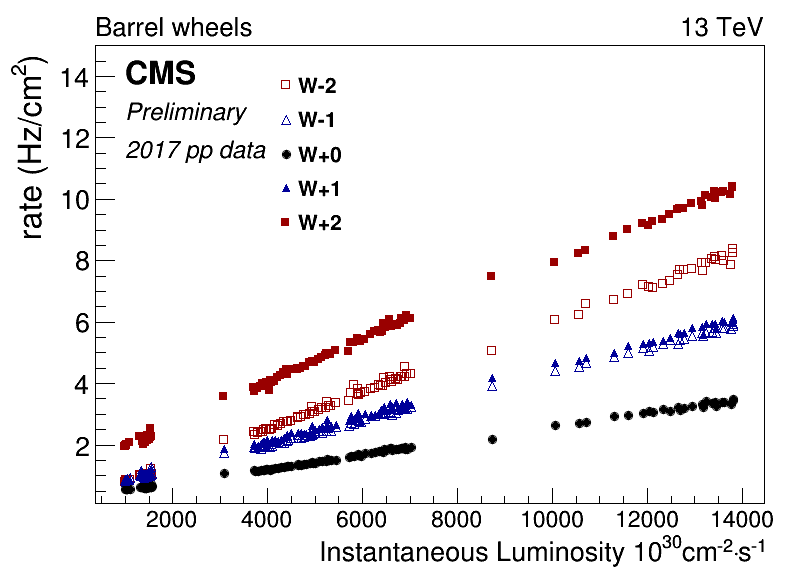
\includegraphics[height=4.3cm]{fig/chapt5/Rate-vs-Lumi-Barrel.png}
			\caption{\label{fig:Rate-I-vs-Lumi:A}}
		\end{subfigure}
		\begin{subfigure}{0.5\linewidth}
			\centering
			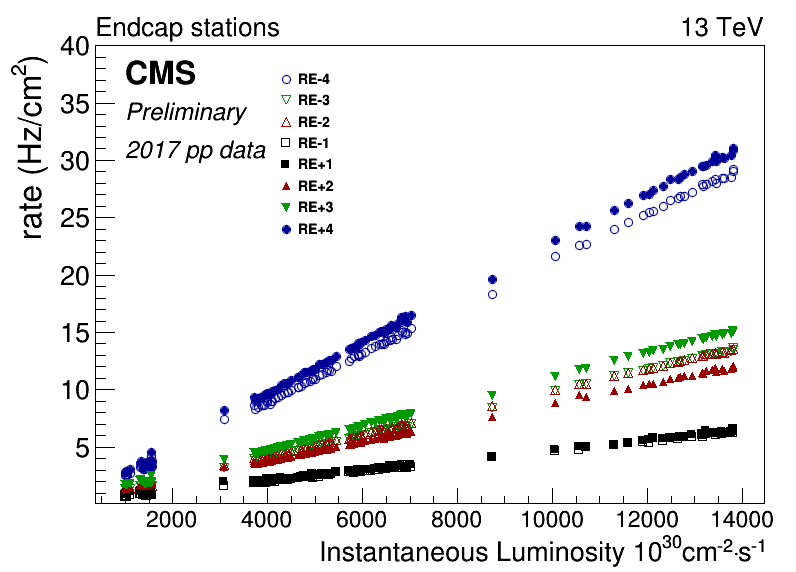
\includegraphics[height=4.3cm]{fig/chapt5/Rate-vs-Lumi-Endcap.png}
			\caption{\label{fig:Rate-I-vs-Lumi:B}}
		\end{subfigure}
		\begin{subfigure}{0.5\linewidth}
			\centering
			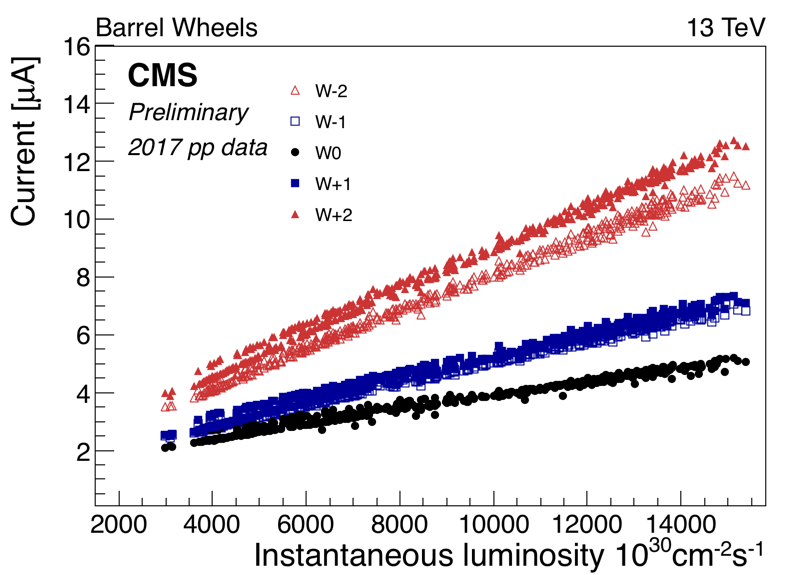
\includegraphics[height=4.3cm]{fig/chapt5/Current-vs-Lumi-Barrel.png}
			\caption{\label{fig:Rate-I-vs-Lumi:C}}
		\end{subfigure}
		\begin{subfigure}{0.5\linewidth}
			\centering
			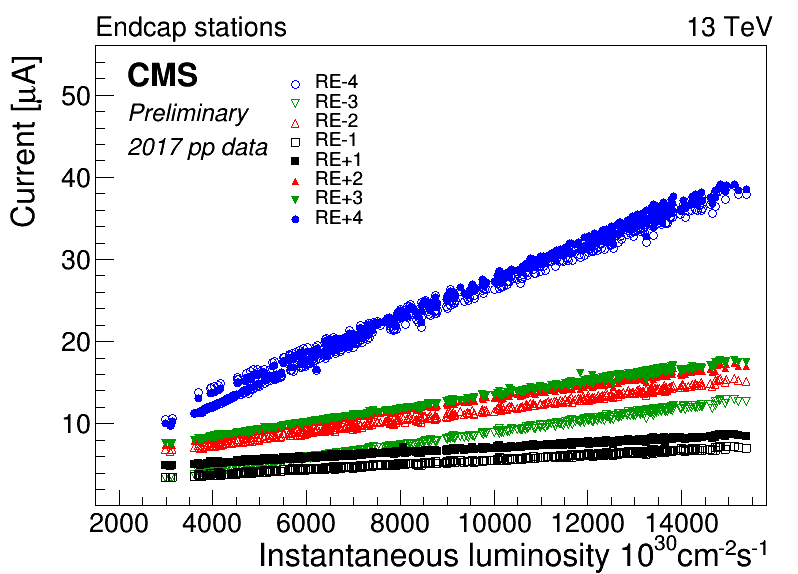
\includegraphics[height=4.3cm]{fig/chapt5/Current-vs-Lumi-Endcap.png}
			\caption{\label{fig:Rate-I-vs-Lumi:D}}
		\end{subfigure}
		\caption{\label{fig:Rate-I-vs-Lumi} Mean RPC Barrel (left column) and Endcap (right column) rate (top row) and current (bottom row) as a function of the instantaneous luminosity as measured in 2017 $p$-$p$ collision data.}
	\end{figure}
	
\begingroup\setlength{\intextsep}{0pt}\setlength{\columnsep}{15pt}
	
	\begin{wrapfigure}{O}{.5\linewidth}
		\begin{subfigure}{\linewidth}
			\centering
			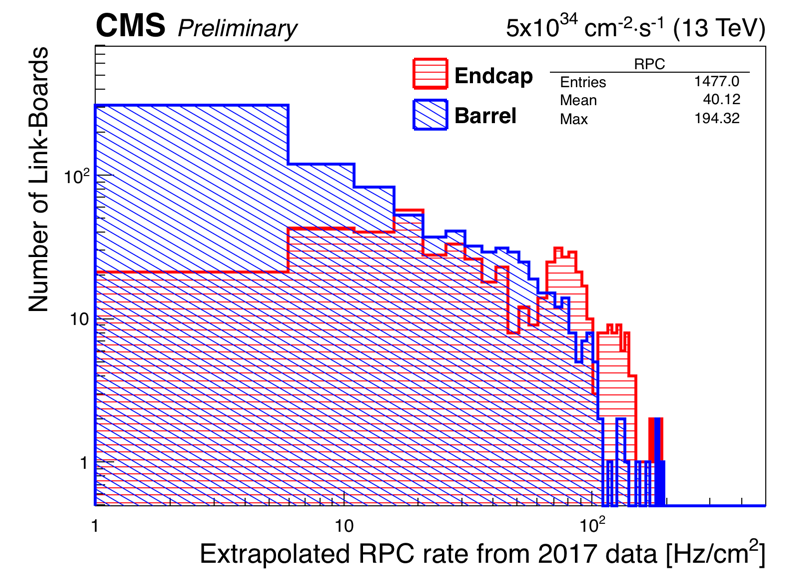
\includegraphics[width=\linewidth]{fig/chapt5/RPC-Rate-HL-LHC_2017.png}
			\caption{\label{fig:RPC-HL-LHC:A}}
		\end{subfigure}
		\begin{subfigure}{\linewidth}
			\centering
			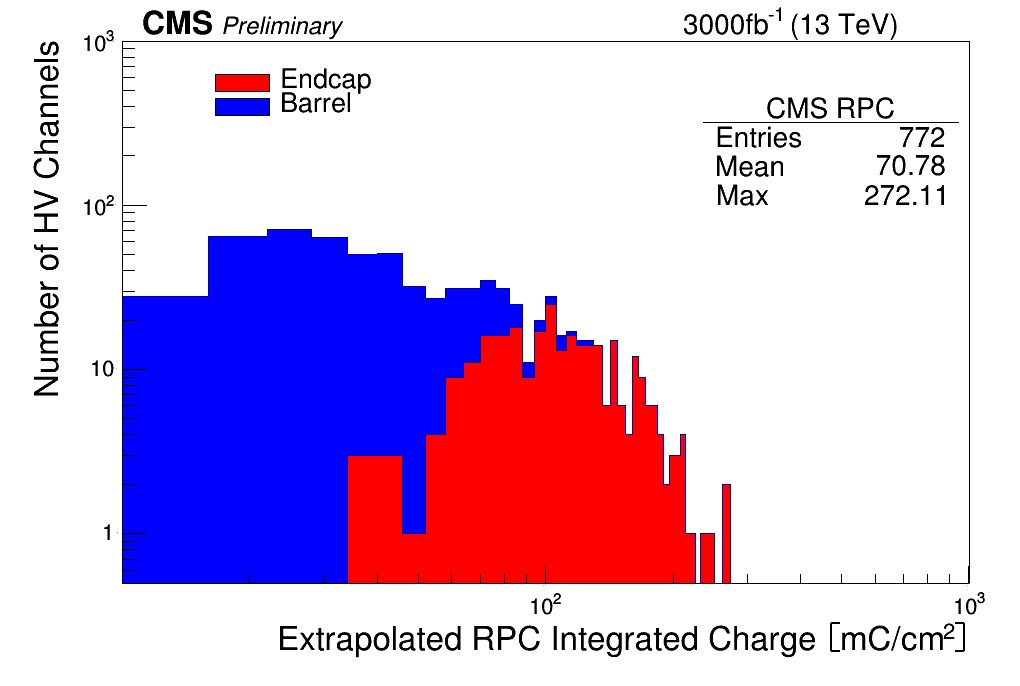
\includegraphics[width=\linewidth]{fig/chapt5/RPC-IC-HL-LHC_2016.png}
			\caption{\label{fig:RPC-HL-LHC:B}}
		\end{subfigure}
		\caption{\label{fig:RPC-HL-LHC} Linear extrapolation of the hit rate \subref{fig:RPC-HL-LHC:A} and of the integrated charge \subref{fig:RPC-HL-LHC:B} per region (Barrel, Endcap) respectively to HL-LHC instantaneous luminosity (\Sci{5}{34} \siflux) and HL-LHC integrated luminosity (\SI{3000}{fb^{-1}}).}
	\end{wrapfigure}

	The upgrade from LHC to HL-LHC will increase the peak luminosity from \Ord{34} \siflux to \Sci{5}{34} \siflux, increasing the total expected background to which the RPC system will be subjected. Mainly composed of low energy gammas, neutrons, and electrons and positrons from $p$-$p$ collisions, but also of low momentum primary and secondary muons, punch-through hadrons from calorimeters, and particles produced in the interaction of the beams with collimators, the background will mostly affect the regions of CMS that are the closest to the beam line, i.e. the RPC detectors located in the endcaps.

	Data collected during 2017, presented in Figure~\ref{fig:Rate-I-vs-Lumi}, allows to study the values of the background rate in the entire RPC system. This was achieved thanks via the monitoring of the rates in each RPC rolls and of the current in each HV channel. A linear dependence of the mean rate or current on the instantaneous luminosity is shown in selected runs with identical LHC running parameters. It is assumed that such a linear behaviour should be observed at even higher luminosities and is therefore used to extrapolates the rates and currents that will be expected during HL-LHC. In Figure~\ref{fig:RPC-HL-LHC}, a linear extrapolation of the distribution of the background hit rate per unit area as well as the integrated charge is showen at a HL-LHC condition. The maximum hit rate per unit area in the endcap detectors at HL-LHC conditions is expected to be of the order of \SIrate{600} while the charge deposition should exceed \SI{800}{mC/cm^2}. The detectors will thus have to be certified up to an irradiation of \SI{840}{mC/cm^2}. These extrapolations are provided with a required safety factor 3 for the certification study.

	In the past, extensive long-term tests were carried out at several gamma and neutron facilities certifying the detector performance. Both full size and small prototype RPCs have been irradiated with photons up to an integrated charge of $\sim$\SI{0.05}{C/cm^2} and $\sim$\SI{0.4}{C/cm^2} respectively and were certified for rates reaching \SIrate{200}~\cite{GIF2004,AGING2009}. Since the beginning of Run-I until December 2017, the RPC system provided stable operation and excellent performance. The average integrated charge is of about \SI{1.66}{mC/cm^2} in the Barrel and \SI{4.58}{mC/cm^2} in the Endcap, closer to the beam line, as can be seen in Figure~\ref{fig:Mean-Int-Charge}). The detectors did not show any ageing effects for a maximum integrated charge in a detector of the order of \SI{0.01}{C/cm^2} and a peak luminosity reaching \Sci{1.4}{34} \siflux during the 2017 data taking period.

\endgroup
	
	To perform the necessary studies on the present CMS RPC detectors, facilities offering the possibility to irradiate the chambers are necessary in order to recreate HL-LHC conditions or stronger and study the detector performance through time. A first series of such studies was conducted in the former \acf{GIF} of CERN before its dismantlement starting from September 2014. This preliminary study was used as a stepping stone towards the building of a more powerful irradiation fully dedicated to longevity studies of CMS and ATLAS subsystems in the perspective of HL-LHC. The period of preliminary work has also been a key moment in the elaboration and improvement of data acquisition, offline analysis and online monitoring tools that are extensively used in the new gamma irradiation facility.
    
	\begin{figure}[H]
		\begin{subfigure}{0.5\linewidth}
			\centering
			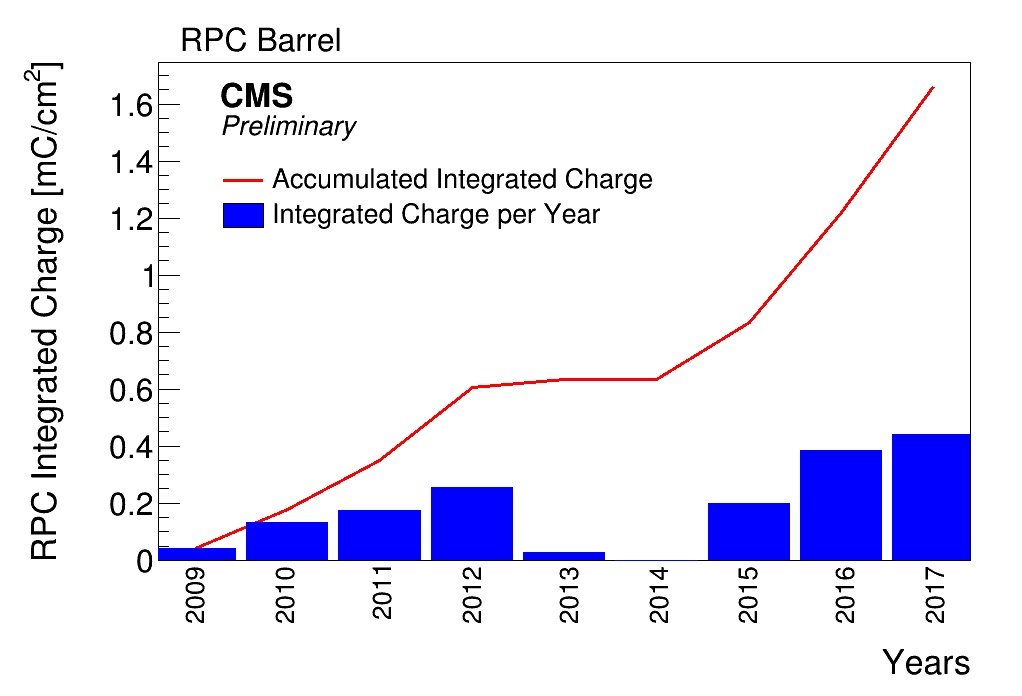
\includegraphics[height=42mm]{fig/chapt5/Mean-Int-charge-Barrel.png}
			\caption{\label{fig:Mean-Int-Charge:A}}
		\end{subfigure}
		\begin{subfigure}{0.5\linewidth}
			\centering
			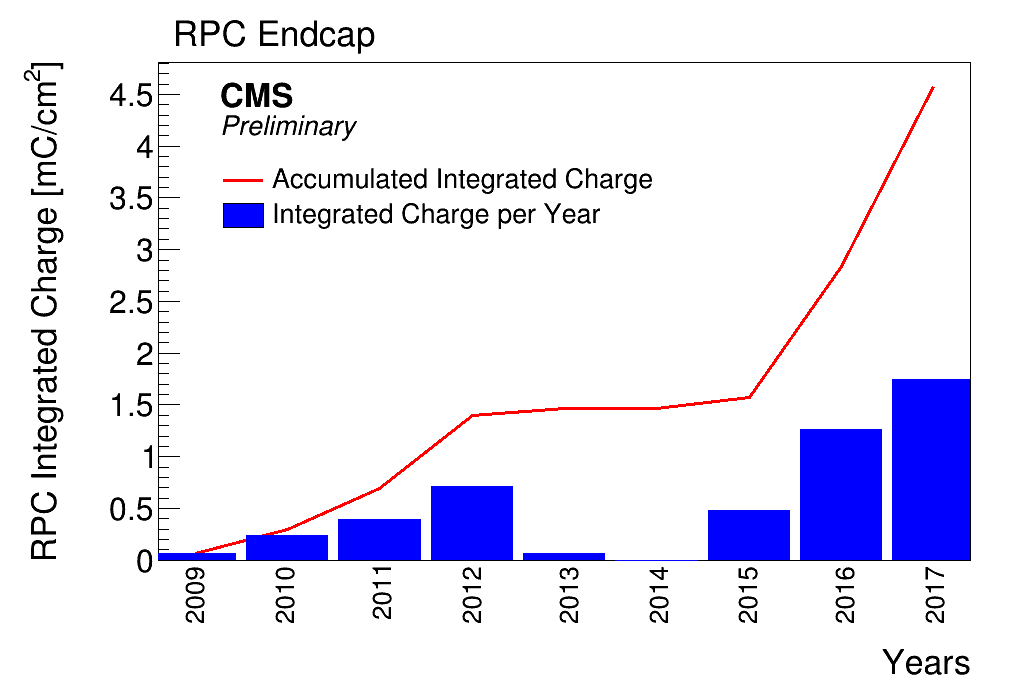
\includegraphics[height=42mm]{fig/chapt5/Mean-Int-charge-Endcap.png}
			\caption{\label{fig:Mean-Int-Charge:B}}
		\end{subfigure}
		\caption{\label{fig:Mean-Int-Charge} CMS RPC mean integrated charge in the Barrel region~\subref{fig:Mean-Int-Charge:A} and the Endcap region~\subref{fig:Mean-Int-Charge:B}. The integrated charge per year is shown in blue. The red curve shows the evolution of the accumulated integrated charge through time. The blank period in 2013 and 2014 corresponds to LS1.}
	\end{figure}
	
		\subsection{The \acl{GIF}}
		\label{chapt5:ssec:GIF}
	
	\begin{figure}[H]
		\centering
		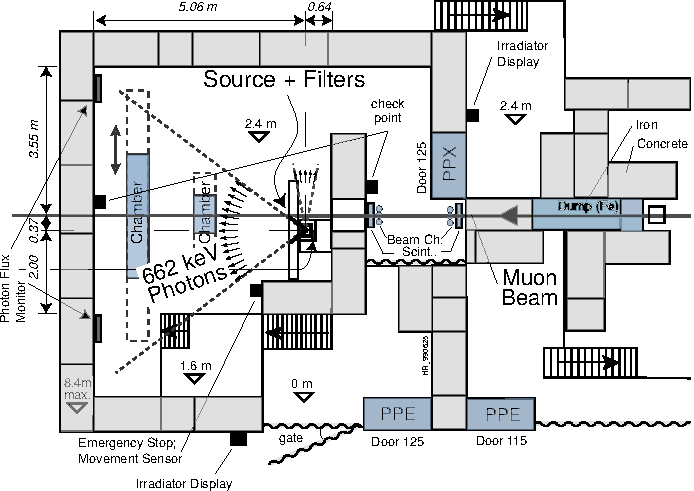
\includegraphics[width = .8\linewidth]{fig/chapt5/GIF-Layout.pdf}\\
		\caption{\label{fig:GIFLayout} Layout of the test beam zone of GIF at CERN.}
	\end{figure}
	
\begingroup\setlength{\intextsep}{5pt}\setlength{\columnsep}{15pt}
	
	\begin{wrapfigure}{O}{.6\linewidth}
		\centering
		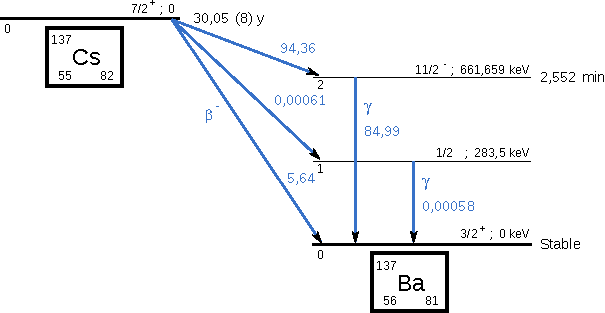
\includegraphics[width = \linewidth]{fig/chapt5/Cs137.pdf}\\
		\caption{\label{fig:CsSource} $^{137}$Cs decays by $\beta^-$ emission to the ground state of $^{137}$Ba (BR = 5.64\%) and via the \SI{662}{keV} isomeric level of $^{137}$Ba (BR = 94.36\%) whose half-life is 2.55min.}
	\end{wrapfigure}
		
	Located in the SPS West Area at the downstream end of the X5 test beam, the GIF was a test area in which particle detectors were exposed to a particle beam in presence of an adjustable gamma background~\cite{AGOSTEO1999}. Its goal was to reproduce background conditions these detectors would endure in their operating environment at LHC. The layout of the GIF is shown in Figure ~\ref{fig:GIFLayout}. Gamma photons are produced by a strong $^{137}$Cs source installed in the upstream part of the zone inside a lead container. The source container includes a collimator, designed to irradiate a \SIsurface{6}{6}{m} area at \SI{5}{m} maximum distance to the source. A thin lens-shaped lead filter helps providing with a uniform out-coming flux in a vertical plane, orthogonal to the beam direction. The photon rate is controlled by further lead filters allowing the maximum rate to be limited and to vary within a range of four orders of magnitude. Particle detectors under test are then placed within the pyramidal volume in front of the source, perpendicularly to the beam line in order to profit from the homogeneous photon flux. Adjusting the background flux of photons can then be done using the filters and choosing the position of the detectors with respect to the source. The zone is surrounded by \SI{8}{m} high and \SI{80}{cm} thick concrete walls. Access is possible through three entry points. Two access doors for personnel and one large gate for material. A crane allows installation of heavy equipment in the area.
	
\endgroup
			
	As described on Figure~\ref{fig:CsSource}, the $^{137}$Cs source emits a \SI{662}{keV} photon in 85\% of the decays. An activity of \SI{740}{GBq} was measured on the \Th{5} of March 1997. The half-life of Cesium is well known ($t_{1/2}=$ \SIerror{30.05}{0.08}{y}) and can be used to compute the activity of the source at the time of the study. The GIF tests were done in between the \Th{20} and the \St{31} of August 2014, i.e. at a time $t=$ \SIerror{17.47}{0.02}{y} resulting in an attenuation of the activity from \SI{740}{GBq} in 1997 to \SI{494}{GBq} in 2014.
		
		\subsection{The \acl{GIF++}}
		\label{chapt5:ssec:GIF++}
		
	The GIF++, located in the SPS North Area at the downstream end of the H4 test beam, has replaced its predecessor during LS1 and has been operational since spring 2015~\cite{JAKEL2014}. Like GIF, GIF++ features a $^{137}$Cs source of \SI{662}{keV} gamma photons, their fluence being controlled with a set of filters of various attenuation factors. The source provides two separate large irradiation areas for testing several full-size muon detectors with homogeneous irradiation, as presented in Figure~\ref{fig:GIFpp-Layout}.
	
	The source activity was measured to be about \SI{13.5}{TBq} in March 2016. With the photon flux being far greater than HL-LHC expectations, GIF++ provides an excellent facility for accelerated ageing tests of muon detectors. The source is situated in a bunker designed to perform irradiation test along a muon beam line, which is available during selected periods throughout the year. The H4 beam, providing the area with muons with a maximum momentum of about \SI{150}{GeV/c}, passes through the GIF++ zone and is used to periodically study the performance of the detectors placed under long term irradiation. Its flux is of \SI{104}{particles/s/\square\cm} focused in an area of about \SIsurface{10}{10}{cm}.
	
\begingroup\setlength{\intextsep}{0pt}\setlength{\columnsep}{15pt}
	
	\begin{wraptable}{O}{.3\linewidth}
		\centering
		\begin{tabular}{c|c|c|c|}
		\cline{2-4}
		 & 1 & 2 & 3 \\
		\hline
		\multicolumn{1}{|c|}{A} & 1 & 10 & 100\\
		\hline
		\multicolumn{1}{|c|}{B} & 1 & 1.468 & 100\\
		\hline
		\multicolumn{1}{|c|}{C} & 1 & 2.154 & 4.642\\
		\hline
		\end{tabular}
		\caption{\label{tab:ABS-GIFpp} Attenuation of single filters on each filter plane of the GIF++ Cesium source.}
	\end{wraptable}
	 
	Adjusting the gamma flux is possible thanks to the three planes (A, B and C) of adjustable absorbers featured on the Cesium source~\cite{GIFFILTERS}. With properly adjusted filters, one can simulate the background expected at HL-LHC and study the performance and ageing of muon detectors in HL-LHC environment. Each plane of filters features three filters (1, 2 and 3) with different \acf{ABS} listed in Table~\ref{tab:ABS-GIFpp}. The source absorber settings can be referred by a three digit number with a format ABC or by its attenuation factor (for example $333 = 100\times 100 \times 4.642 = 46420$).
	
\endgroup
	
	\begin{figure}[H]
		\centering
		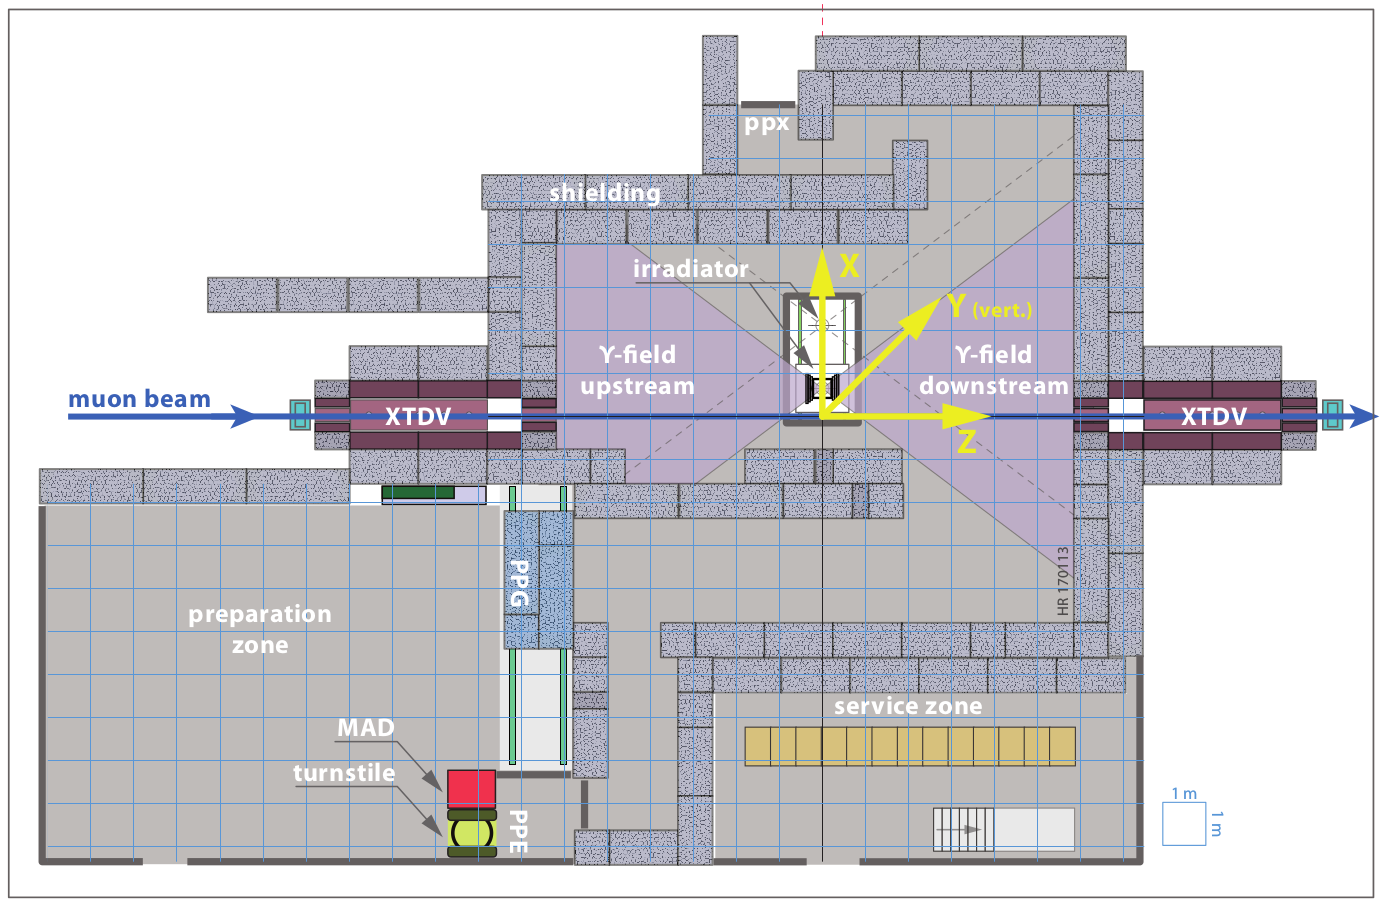
\includegraphics[width = .75\linewidth]{fig/chapt5/GIFpp-Layout.png}\\
		\caption{\label{fig:GIFpp-Layout} Floor plan of the GIF++ facility. When the facility downstream of the GIF++ takes electron beam, a beam pipe is installed along the beam line (z-axis). The irradiator can be displaced laterally (its center moves from $x=$ \SI{0.65}{m} to \SI{2.15}{m}), to increase the distance to the beam pipe.}
	\end{figure}
	 
	\begin{figure}[H]
		\begin{subfigure}{0.5\linewidth}
		    \centering
			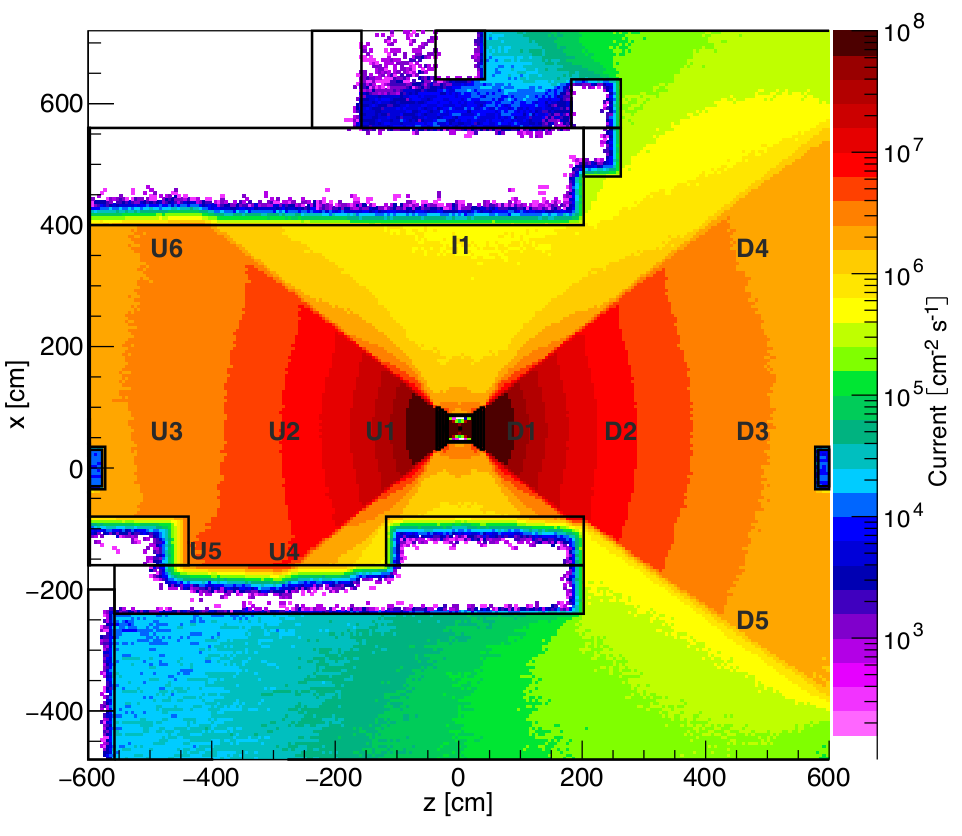
\includegraphics[width = .85\linewidth]{fig/chapt5/GIFpp-gCurrent-XZ.png}\\
			\caption{\label{fig:GIFpp-gCurrent:XZ}}
		\end{subfigure}
		\begin{subfigure}{0.5\linewidth}
		    \centering
			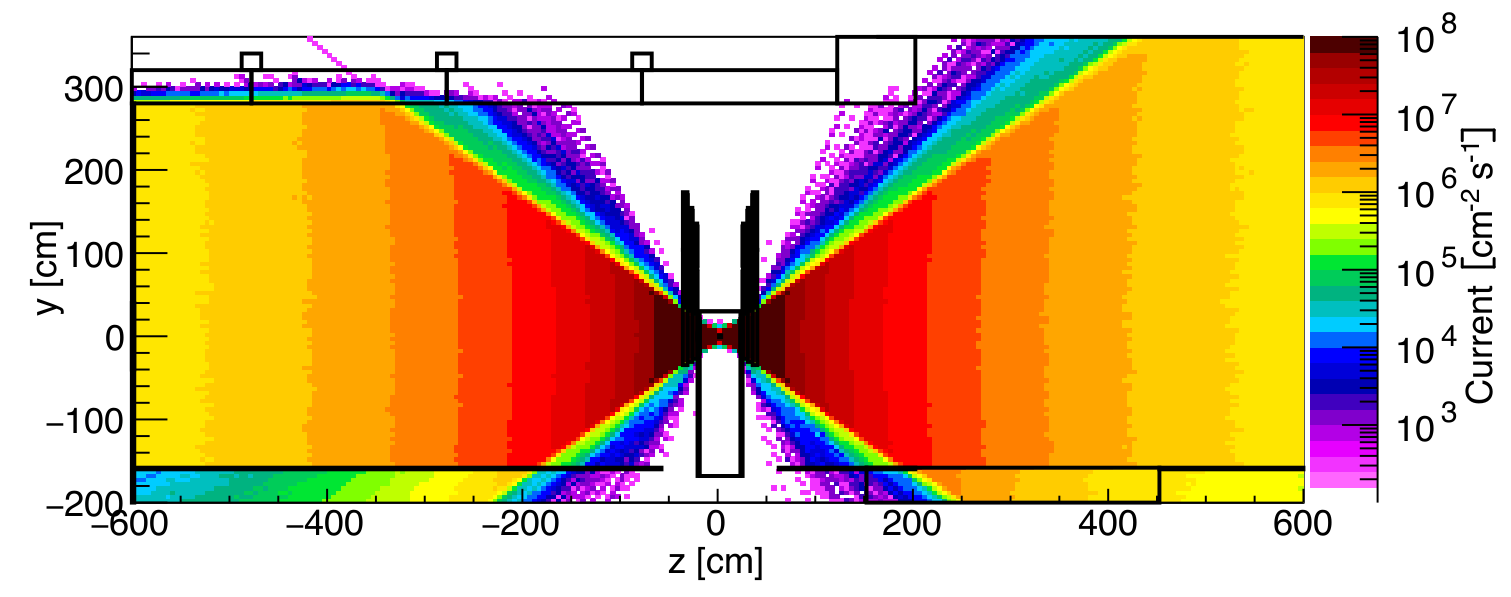
\includegraphics[width = .85\linewidth]{fig/chapt5/GIFpp-gCurrent-YZ.png}
			\caption{\label{fig:GIFpp-gCurrent:YZ}}
		\end{subfigure}
		\caption{\label{fig:GIFpp-gCurrent} Simulated unattenuated current of photons in the xz plane~\subref{fig:GIFpp-gCurrent:XZ} and yz plane~\subref{fig:GIFpp-gCurrent:YZ} through the source at $x=$ \SI{0.65}{m} and $y=$ \SI{0}{m}~\cite{PFEIFFER2017}. With angular correction filters, the current of \SI{662}{keV} photons is made uniform in xy planes.}
    \end{figure}
	
	The gamma current as simulated with GEANT4 is presented in Figure~\ref{fig:GIFpp-gCurrent}. In their simulation paper~\cite{PFEIFFER2017}, Pfeiffer et al. define the particle current as \textit{"a measure of the net number of particles crossing a flat surface with a well-defined orientation. The unit of current is \si{m^{-2}.s^{-1}} and thus identical to the unit of flux. Current is meaningful in cases where particles are counted without any interest in their interactions."} The labels U$N$, D$N$, with $N \in [1:5]$ and I1 correspond to the position of different \acf{RADMON} sensors measuring the irradiation in the bunker area~\cite{PFEIFFER2017}. According to the simulation results, that agree within 12\% to the doses measured with the RADMONs, the RPCs that will be tested in GIF++ can expect a maximal gamma current of the order of 2 to \Sci{5}{6} \siflux assuming they will always stay in a region in between sensor U5 and the back wall of the upstream area.
	 
\section{Preliminary studies at GIF}
\label{chapt5:sec:GIFtests}

	\subsection{RPC test setup}
	\label{chapt5:ssec:RPCSetup}

	\begin{figure}[H]
		\begin{subfigure}{0.5\linewidth}
		    \centering
			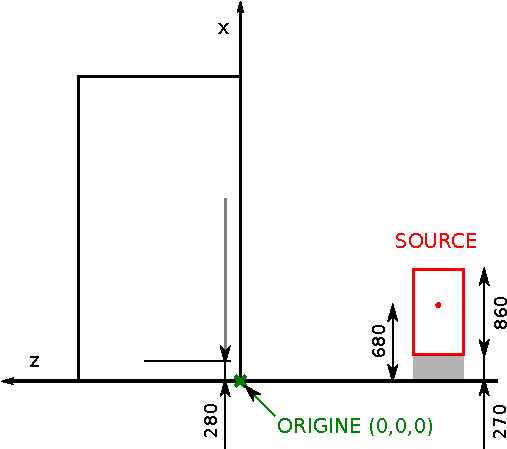
\includegraphics[width = .8\linewidth]{fig/chapt5/GIF-Setup-A.pdf}
			\caption{\label{fig:GIFSetup:A}}
		\end{subfigure}
		\begin{subfigure}{0.5\linewidth}
		    \centering
			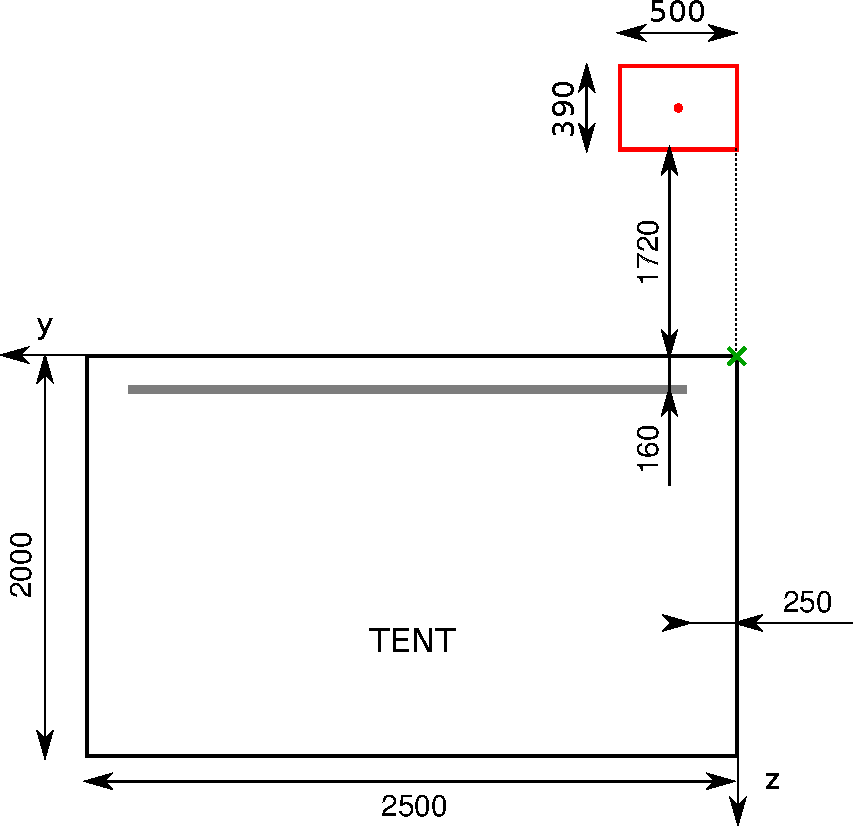
\includegraphics[width = .8\linewidth]{fig/chapt5/GIF-Setup-B.pdf}
			\caption{\label{fig:GIFSetup:B}}
		\end{subfigure}
		\caption{\label{fig:GIFSetup} Description of the RPC setup. Dimensions are given in \si{mm}. A tent containing RPCs is placed at \SI{1720}{mm} from the source container. The source is situated in the center of the container. RE-4-2-BARC-161 chamber is \SI{160}{mm} inside the tent. This way, the distance between the source and the chambers plan is \SI{2060}{mm}. Figure~\subref{fig:GIFSetup:A} provides a side view of the setup in the $xz$ plane while Figure~\subref{fig:GIFSetup:B} shows a top view in the $yz$ plane.}
	\end{figure}
	
	During Summer 2014, preliminary tests have been conducted in the GIF area on an endcap chamber of type RE4/2 and labeled \texttt{RE-4-2-BARC-161} produced for the extension of the endcap with a fourth disk in 2013. This chamber has been placed into a trolley covered with a tent in order to control the temperature. The positions of the RPC inside the tent and of the tent with respect to the source in the bunker are described in Figure~\ref{fig:GIFSetup}. The goal of the study was to have a preliminary understanding of the rate capability of the present technology used in CMS. It was decided to measure the efficiency of the RPC under irradiation for detecting cosmic muons as, at the time of the tests, the beam was not operational anymore. Three different absorber settings were used and compared to the case where the detector was not irradiated in order to study the evolution of the performance of the detector with increasing exposure to gamma radiation. First of all, measurements were done with the fully opened source. To complete this preliminary study, the gamma flux has been attenuated by a factor 2, a factor 5 and finally the source was shut down. The efficiency of the RPC at detecting the cosmic muons in coincidence with a cosmic trigger as well as the background rate as seen by the detectors were measured.

	\begin{figure}[H]
		\begin{subfigure}{\linewidth}
			\centering
			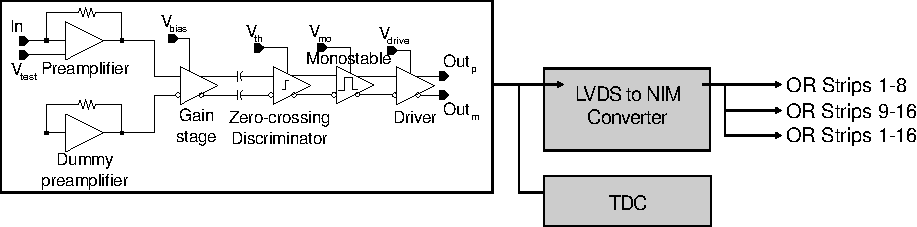
\includegraphics[width = \plotwidth]{fig/chapt5/pulse-processing.pdf}\\
			\caption{\label{fig:DAQ:A}}
		\end{subfigure}
		\begin{subfigure}{\linewidth}
			\centering
			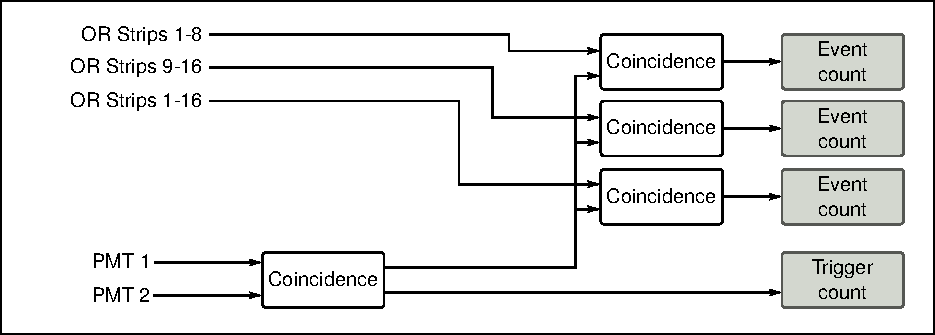
\includegraphics[width = \plotwidth]{fig/chapt5/pulse-processing-2.pdf}
			\caption{\label{fig:DAQ:B}}
		\end{subfigure}
		\caption{\label{fig:DAQ} \subref{fig:DAQ:A} Shaping of the signals from the RPC strips by the FEE. The output LVDS signals are then read-out by a TDC module connected to a computer or converted into NIM and sent to scalers. \subref{fig:DAQ:B} Trigger logic implementation with the RPC and photomulitplier signals.}
	\end{figure}
	
\begingroup\setlength{\intextsep}{5pt}\setlength{\columnsep}{15pt}
	
	\begin{wrapfigure}{O}{.6\linewidth}
		\centering
		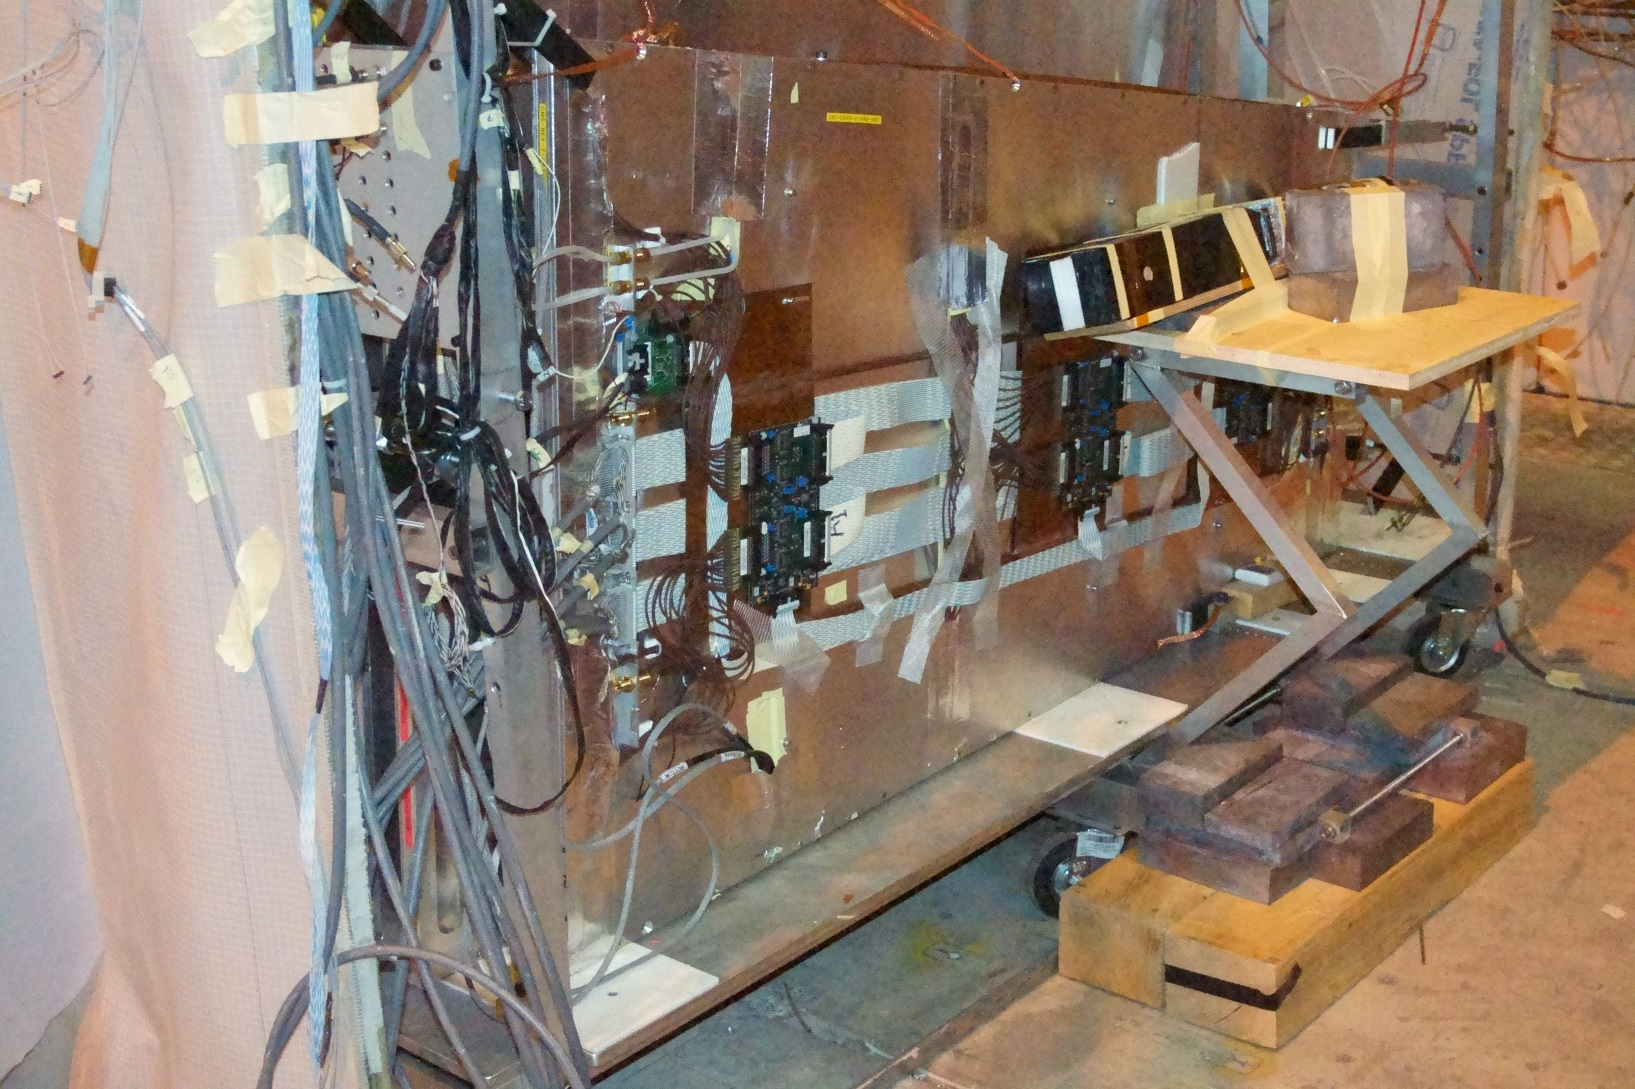
\includegraphics[width = \linewidth]{fig/chapt5/GIF-RPCSetup.jpg}\\
		\caption{\label{fig:GIF-RPCSetup} \texttt{RE-4-2-BARC-161} chamber is inside the tent as described in Figure~\ref{fig:GIFSetup}. In the top right, the two scintillators used as trigger can be seen.}
	\end{wrapfigure}
	
	The data taking was performed using a \texttt{CEAN} TDC module of type \texttt{V1190A}~\cite{V1190AMUT} to which the digitized output of the RPC \acl{FEB} is connected, as described in Figure~\ref{fig:DAQ:A} and the trigger signal from the telescope. The communication with the computer is performed thanks to a \texttt{CAEN} communication module of type \texttt{V1718}~\cite{V1718MUT}. In order to control the rates recorded by the detector, the digitized RPC signals are also sent to scalers as described in Figure~\ref{fig:DAQ:B}. The \texttt{C++} DAQ software used in GIF was developed as an early attempt towards the understanding of the \texttt{CAEN} libraries and the data collected by the TDCs was saved into \texttt{.dat} files is analysed with an algorithm computing parameters such as efficiency, hit profile, cluster size, or gamma and noise rates which was developed with \texttt{C++} as well. Finally, histograms and curves are produced using \texttt{ROOT}.

\endgroup
\newpage
	
\begingroup\setlength{\intextsep}{10pt}\setlength{\columnsep}{15pt}
	
	\begin{wrapfigure}{O}{.6\linewidth}
		\centering
		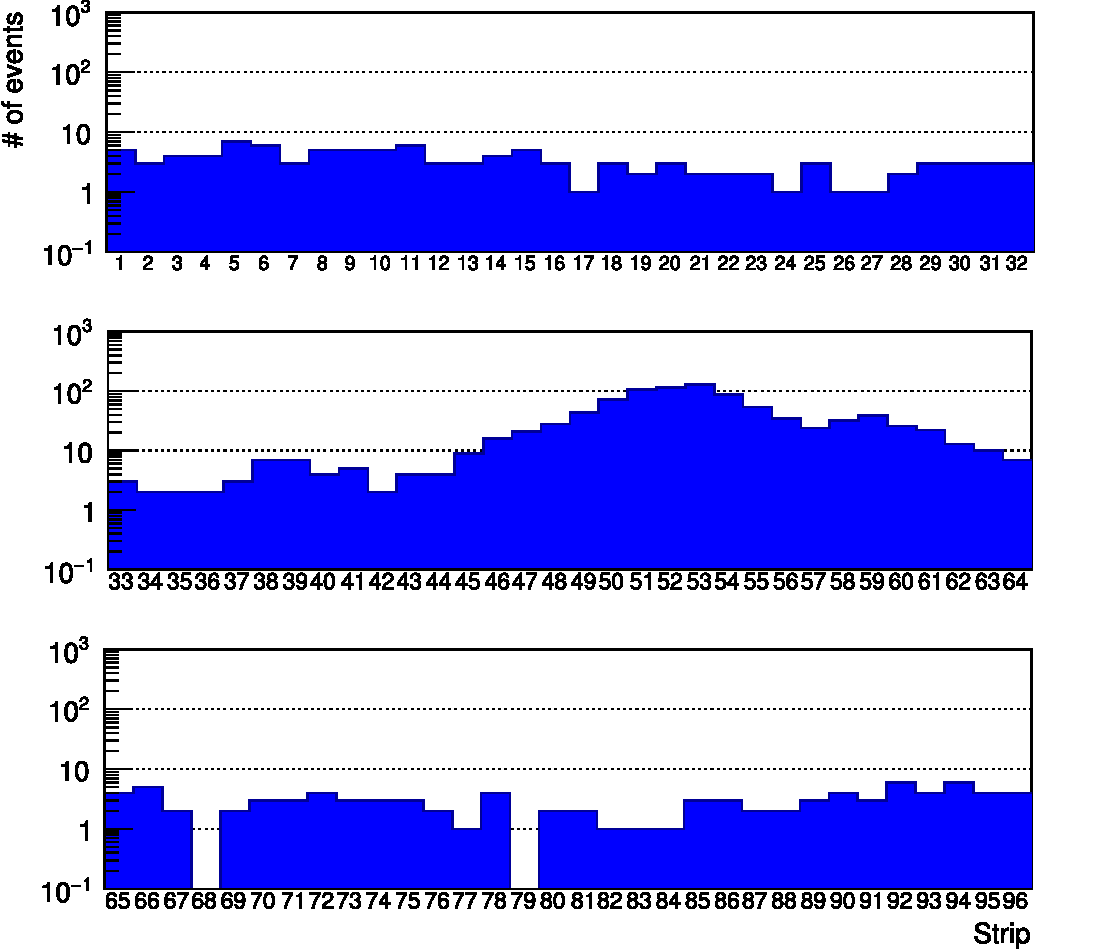
\includegraphics[width = \linewidth]{fig/chapt5/Data-21-profile.pdf}\\
		\caption{\label{fig:HitProf} Hit distributions over all three partitions of \texttt{RE-4-2-BARC-161} chamber is showed. Top, middle and bottom figures respectively correspond to partitions A, B, and C.}
	\end{wrapfigure}
	
	The trigger system was composed of two plastic scintillators and was placed in front of the setup with an inclination of \SI{10}{\degree} with respect to the detector plane in order to look at cosmic muons. Using this particular trigger layout, shown in Figure~\ref{fig:GIF-RPCSetup}, lead to a cosmic muon hit distribution into the chamber similar to the one of Figure~\ref{fig:HitProf}. As mentioned in Chapter~\ref{chapt:2}, the endcap RPC read-out is segmented into three pseudo-rapidity partitions. The outter most partition, corresponding to the wide end of the chamber, is the partition A. The other two partitions are the partitions B and C. Each of them consists in 32 copper strips. These 32 strips are connected to the FEEs by groups of 16. The trigger is placed in fron of the half-partition B2 which corresponds to the last 16 strips of partition B (49 to 64).
	
	Measured without gamma irradiation, two peaks can be seen on the profile of readout partition B, centered on strips 52 and 59. Some events still occur in other half-partitions than B2 contributing to the inefficiency of detection of cosmic muons. In the case of partitions A and C, the very low amount of data can be interpreted as noise. On the other hand, it is clear that a little portion of muons reached the half-partition B1 (strips 33 to 48). Section~\ref{chapt5:ssec:GeoAcc} will help us understand that these two peaks are due respectively to forward and backward coming cosmic particles. Forward coming particles are detected first by the scintillators and then the RPC while the backward going muons are first detected in the RPC.
	
\endgroup
	
	\subsection{Geometrical acceptance of the setup layout to cosmic muons}
	\label{chapt5:ssec:GeoAcc}
				
	In order to profit from a constant gamma irradiation, the detectors inside of the GIF bunker had to be placed in a plane orthogonal to the beam line. The muon beam that used to be available was meant to test the performance of detectors under test. This beam being not active anymore, another solution to test detector performance had to be used. Thus, it was decided to use cosmic muons detected through a telescope composed of two scintillators. Lead blocks were used as shielding to protect the photomultipliers from gammas as can be seen from Figure~\ref{fig:GIF-RPCSetup}.
				
	An inclination of $\sim$\SI{10}{\degree} was given to the cosmic telescope to increase the muon trigger rate for this otherwise horizontal setup. A good compromise had to be found between good enough muon flux and narrow enough hit distribution to be sure to contain all the events into a single half-partition as required from the limited available readout hardware. It was then foreseen to detect muons and read them out only from half-partition B2. Nevertheless, a misplacement of the trigger scintillators resulted in an inefficiency, as can be seen in Figure~\ref{fig:HitProf} with events appearing in half-partition B1.
	
\begingroup\setlength{\intextsep}{5pt}\setlength{\columnsep}{15pt}
	
	\begin{wrapfigure}{O}{.65\linewidth}
            \centering
		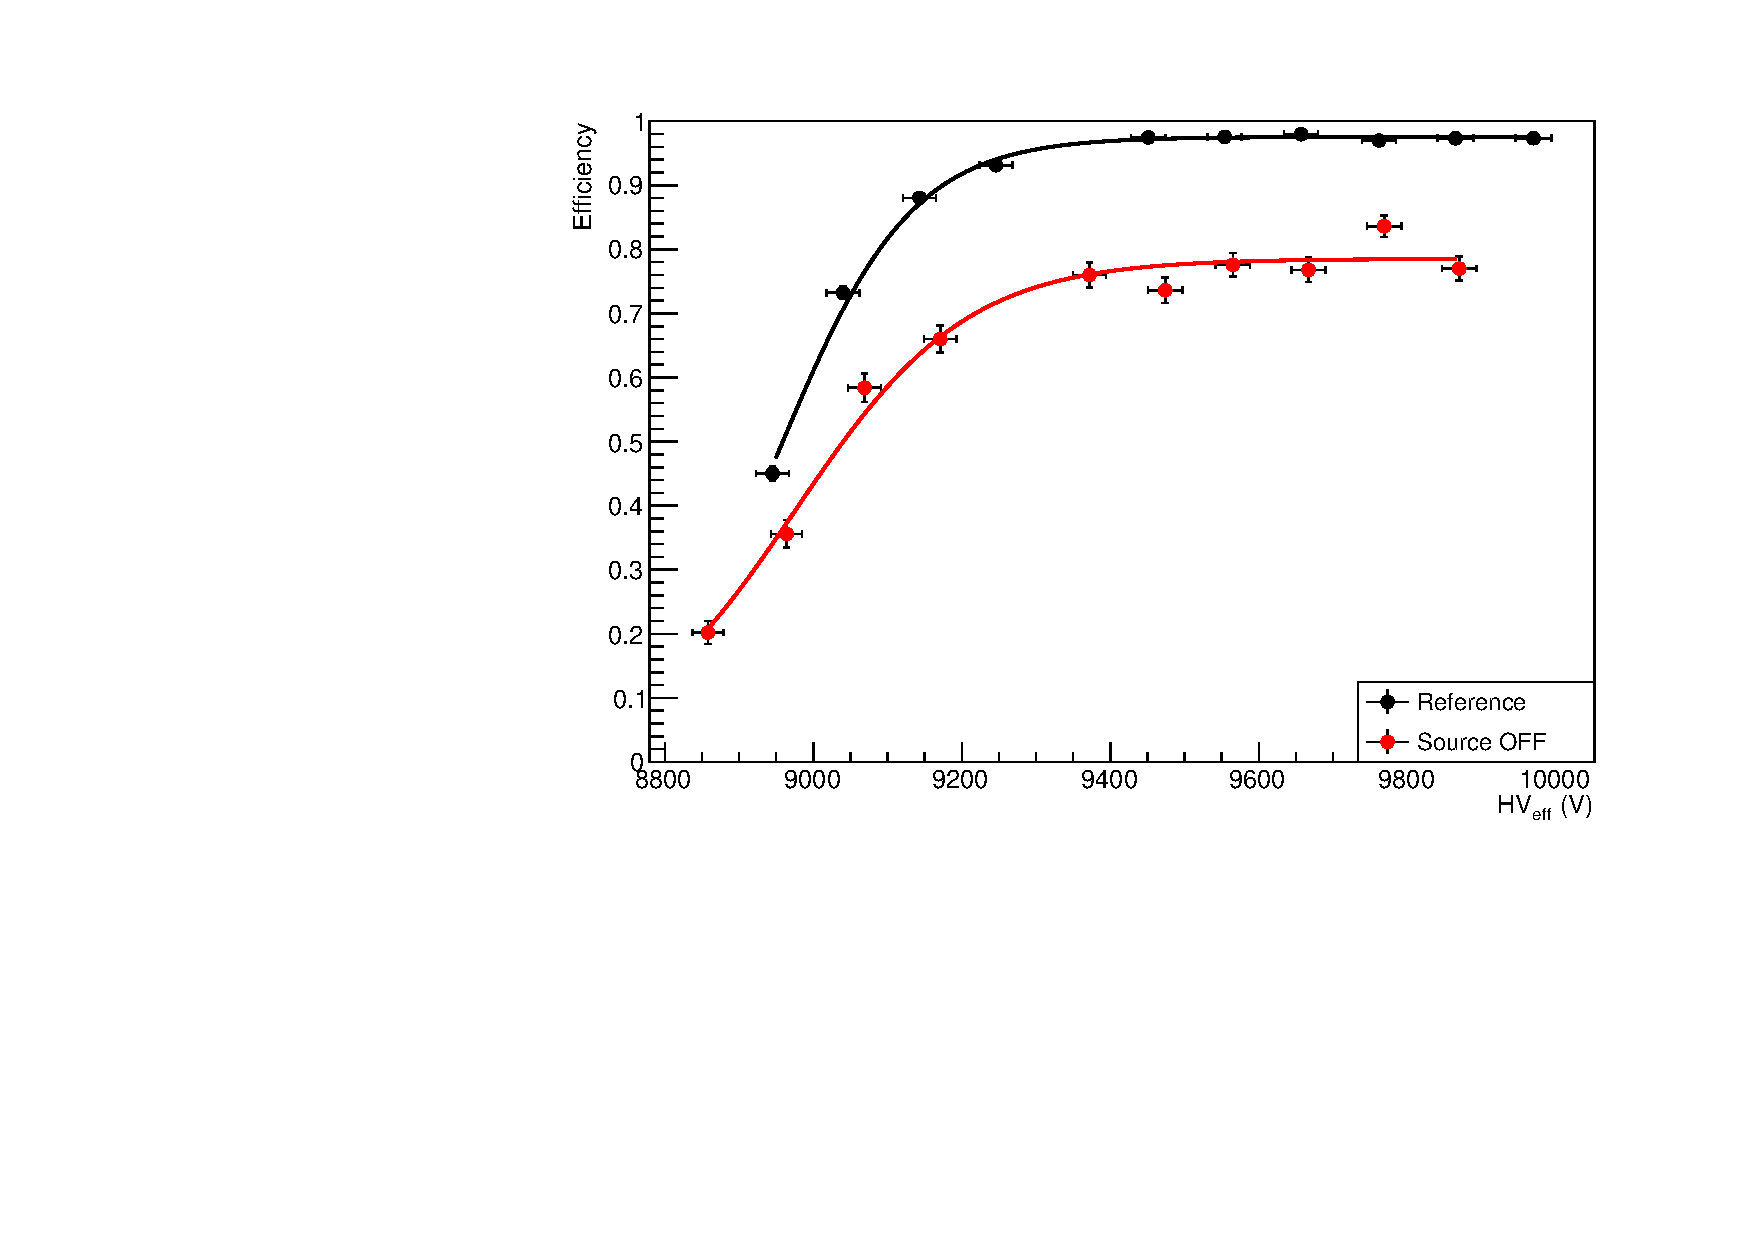
\includegraphics[width = \linewidth]{fig/chapt5/Compared-Efficiency.pdf}
		\caption{\label{fig:EffCompar} Comparison of the efficiency of chamber \texttt{RE-4-2-BARC-161} with and without irradiation. Results are derived from data taken on half-partition B2 only.}
	\end{wrapfigure}
	
	As can be seen in Figure~\ref{fig:EffCompar}, a comparison of the performance of chamber \texttt{RE-4-2-BARC-161} with and without irradiation suggests an inefficiency of approximately 20\%. On the \Th{18} of June 2014, data have been taken on the chamber at CERN building 904 (Prevessin Site) with cosmic muons providing us a reference efficiency plateau of \numerror{97.54}{0.15}\% represented by the black curve. A similar measurement has been done at GIF on the \St{21} of July with the same chamber giving a plateau of \numerror{78.52}{0.94}\% represented by the red curve. The inefficiency too high compared to the 12.7\% of data contained into the first 16 strips observed on Figure~\ref{fig:HitProf}, to be explained only by the geometrical acceptance of the setup itself. Simulations have been conducted to quantify the inefficiency of the setup.
	
\endgroup
		
		\subsubsection{Geometrical acceptance simulation setup}
		\label{chapt5:sssec:GeoSim}
		
	The layout of the GIF setup has been reproduced\footnote{Albeit only roughly using Figure~\ref{fig:GIF-RPCSetup} due to the lack of actual measurements of the respective positions of each parts of the experimental setup. Using reference dimensions such as the saize of the detector and the size of the photomultiplier, the positions could be deduced.} and incorporated into a \texttt{C++} \acf{MC} simulation to study the geometrical acceptance of the telescope projected onto the readout strips~\cite{GEOACCEPT}. A 3D view of the simulated layout is given into Figure~\ref{fig:SimGIFLay}. The RPC read-out plane is represented as a yellow trapezoid while the two scintillators as blue cuboids. The green plane corresponds to the \SIsurface{4}{4.5}{m} muon generation plane centered on the experimental setup within the simulation. The goal of the simulation is to look at muons that pass through the telescope composed of the two scintillators and define their distribution onto the RPC read-out plane. During the reconstruction, the read-out plane is then divided into its read-out strips and each muon track is assigned to a strip.
	
	$N_{\mu}=$ \Ord{8} muons are generated at a random position in the horizontal generation plane. This position corresponds to the intersection of the muon track with the generaltion plane. The plane is located at a height corresponding to the lowest point of the scintillators in order to easily simulate muons coming at very large zenith angles (i.e. $\theta\approx\pi$). The position of the particle within the plane is associated with a random direction: an azimuth angle $\phi$ chosen between 0 and $2\pi$ and a zenith angle $\theta$ chosen between 0 and $\pi/2$ to follow a usual $cos^2\theta$ distribution for cosmic particles. Then, using the position of the muon in the generation plane and its direction, the intersection of the track with the planes of the scintillator cuboids is computed. In the case the muon wasn't found within the surface of both the scintillators, the simulation restarts and generates a new muon. On the contrary, if the track passed through the telescope, the simulation goes on. The position of the muon hit within the RPC read-out plane is computed. The hits are saved into histograms, one per read-out partition, whose bins corresponds to the RPC copper strips. The strip in which the hit occured is determined by knowing precisely the geometry of the RPC. Muon hits are also filled in different histograms whether they are associated to forward coming ($\pi\leq\phi<2\pi$) or backward going ($0\leq\phi<\pi$) muons.

	\begin{figure}[H]
		\begin{subfigure}{\linewidth}
			\centering
			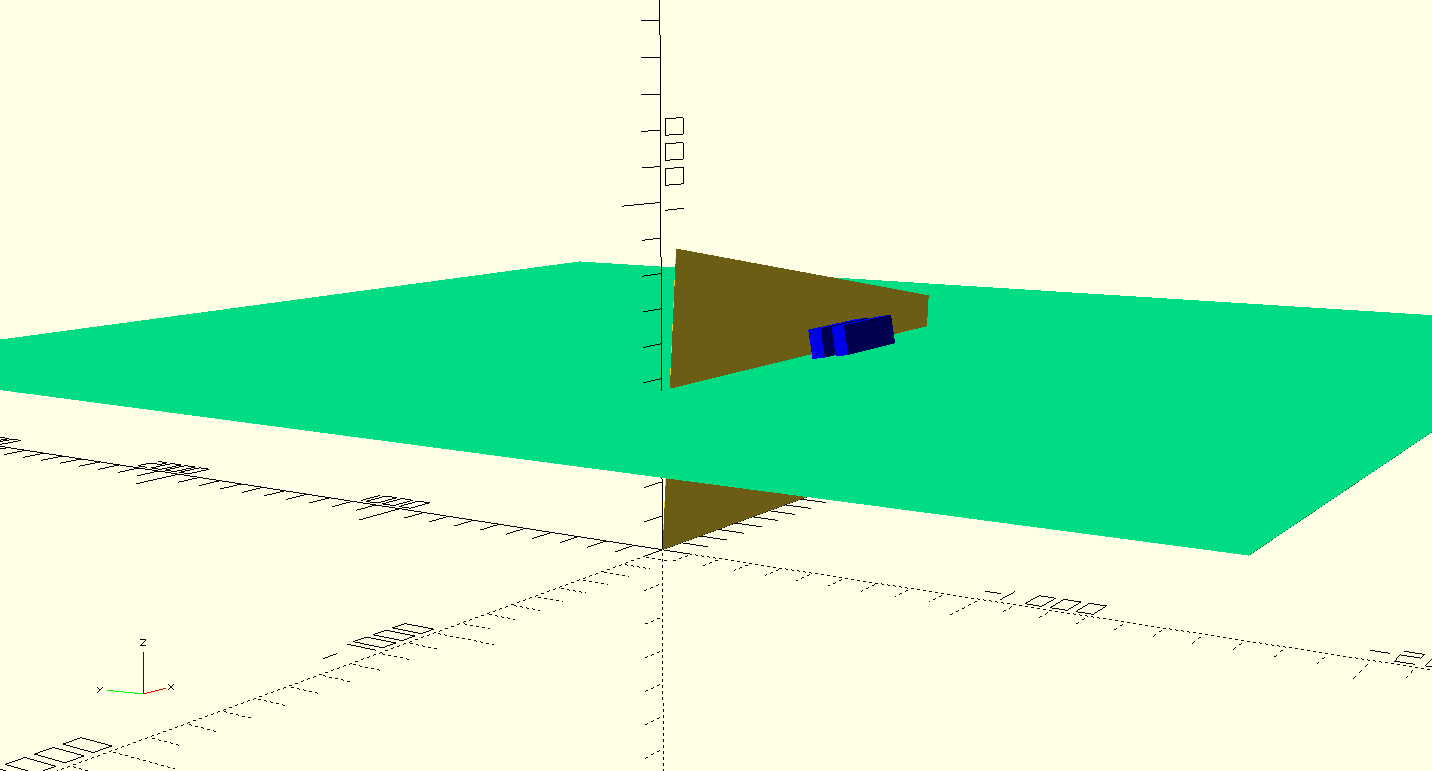
\includegraphics[width = .9\linewidth]{fig/chapt5/GIFSetup-SimA.png}\\
			\caption{\label{fig:SimGIFLay:A}}
		\end{subfigure}
		\begin{subfigure}{\linewidth}
			\centering
			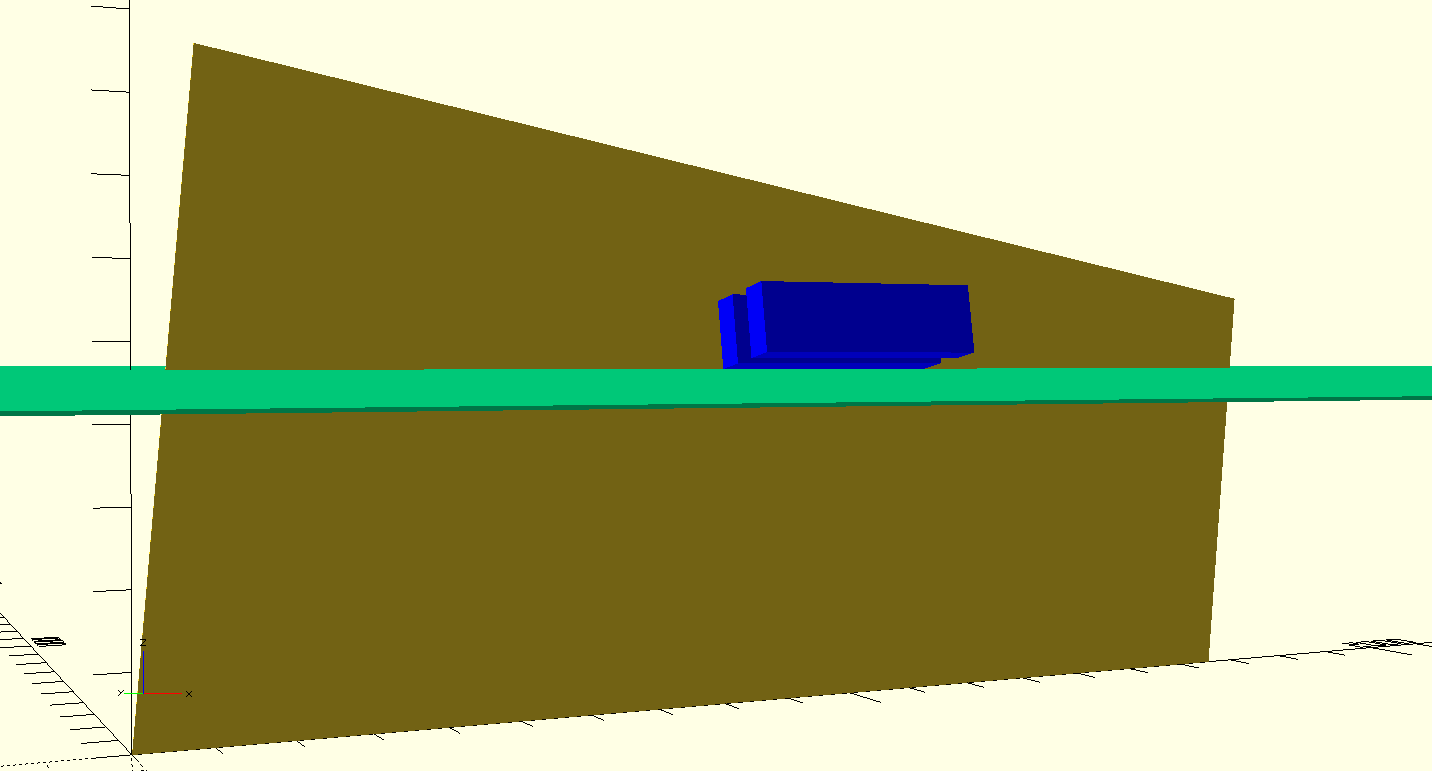
\includegraphics[width = .9\linewidth]{fig/chapt5/GIFSetup-SimB.png}
			\caption{\label{fig:SimGIFLay:B}}
		\end{subfigure}
		\caption{\label{fig:SimGIFLay} Representation of the layout used for the simulations of the test setup. \subref{fig:SimGIFLay:A} Global view of the simulated setup. \subref{fig:SimGIFLay:B} Zoomed view on the experimental setup.}
	\end{figure}

\newpage
		
		\subsubsection{Results and limitations}
		\label{chapt5:sssec:SimRes}
	
\begingroup\setlength{\intextsep}{5pt}\setlength{\columnsep}{15pt}
	
	\begin{wrapfigure}{O}{.5\linewidth}
		\begin{subfigure}{\linewidth}
			\centering
			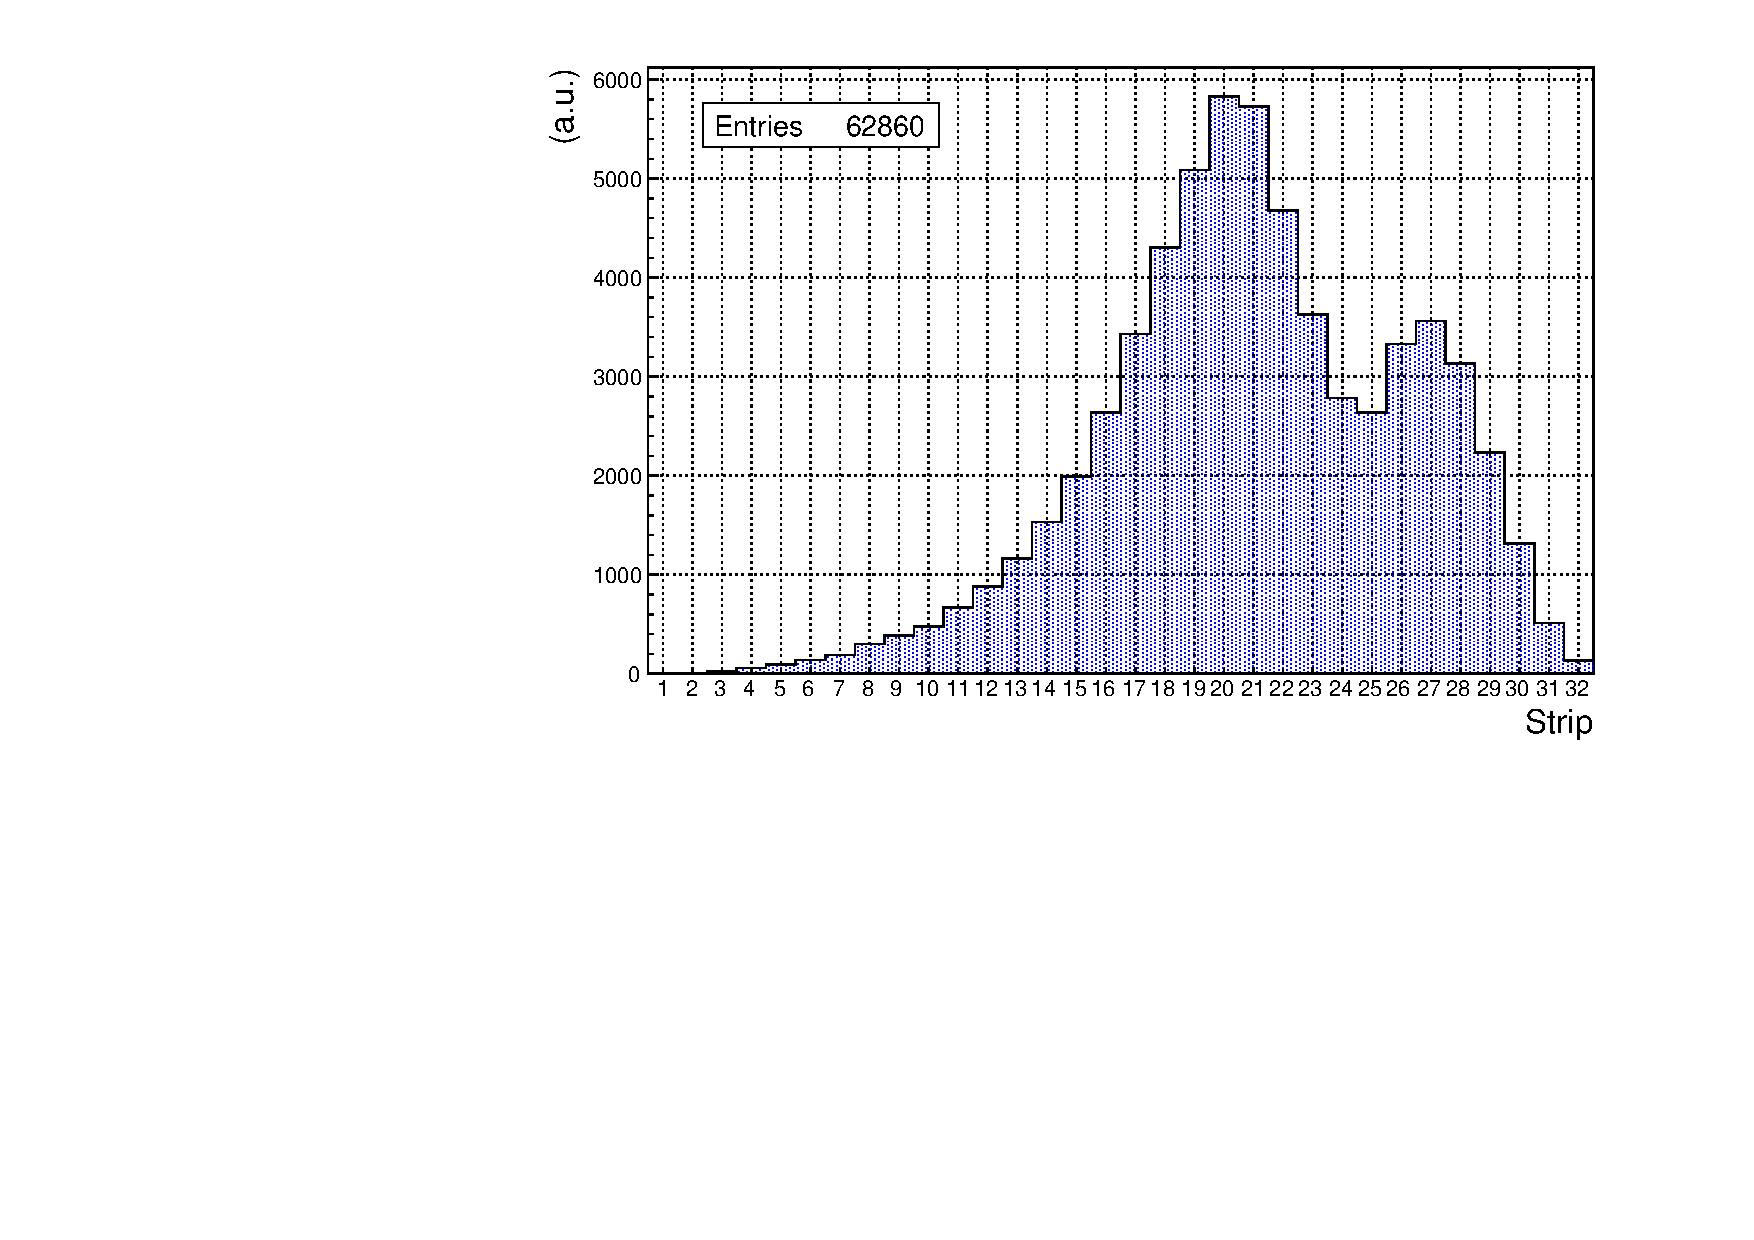
\includegraphics[width = \linewidth]{fig/chapt5/Geometrical-acceptance.pdf}\\
			\caption{\label{fig:SimResult:A} Full acceptance distribution}
		\end{subfigure}
		\begin{subfigure}{\linewidth}
			\centering
			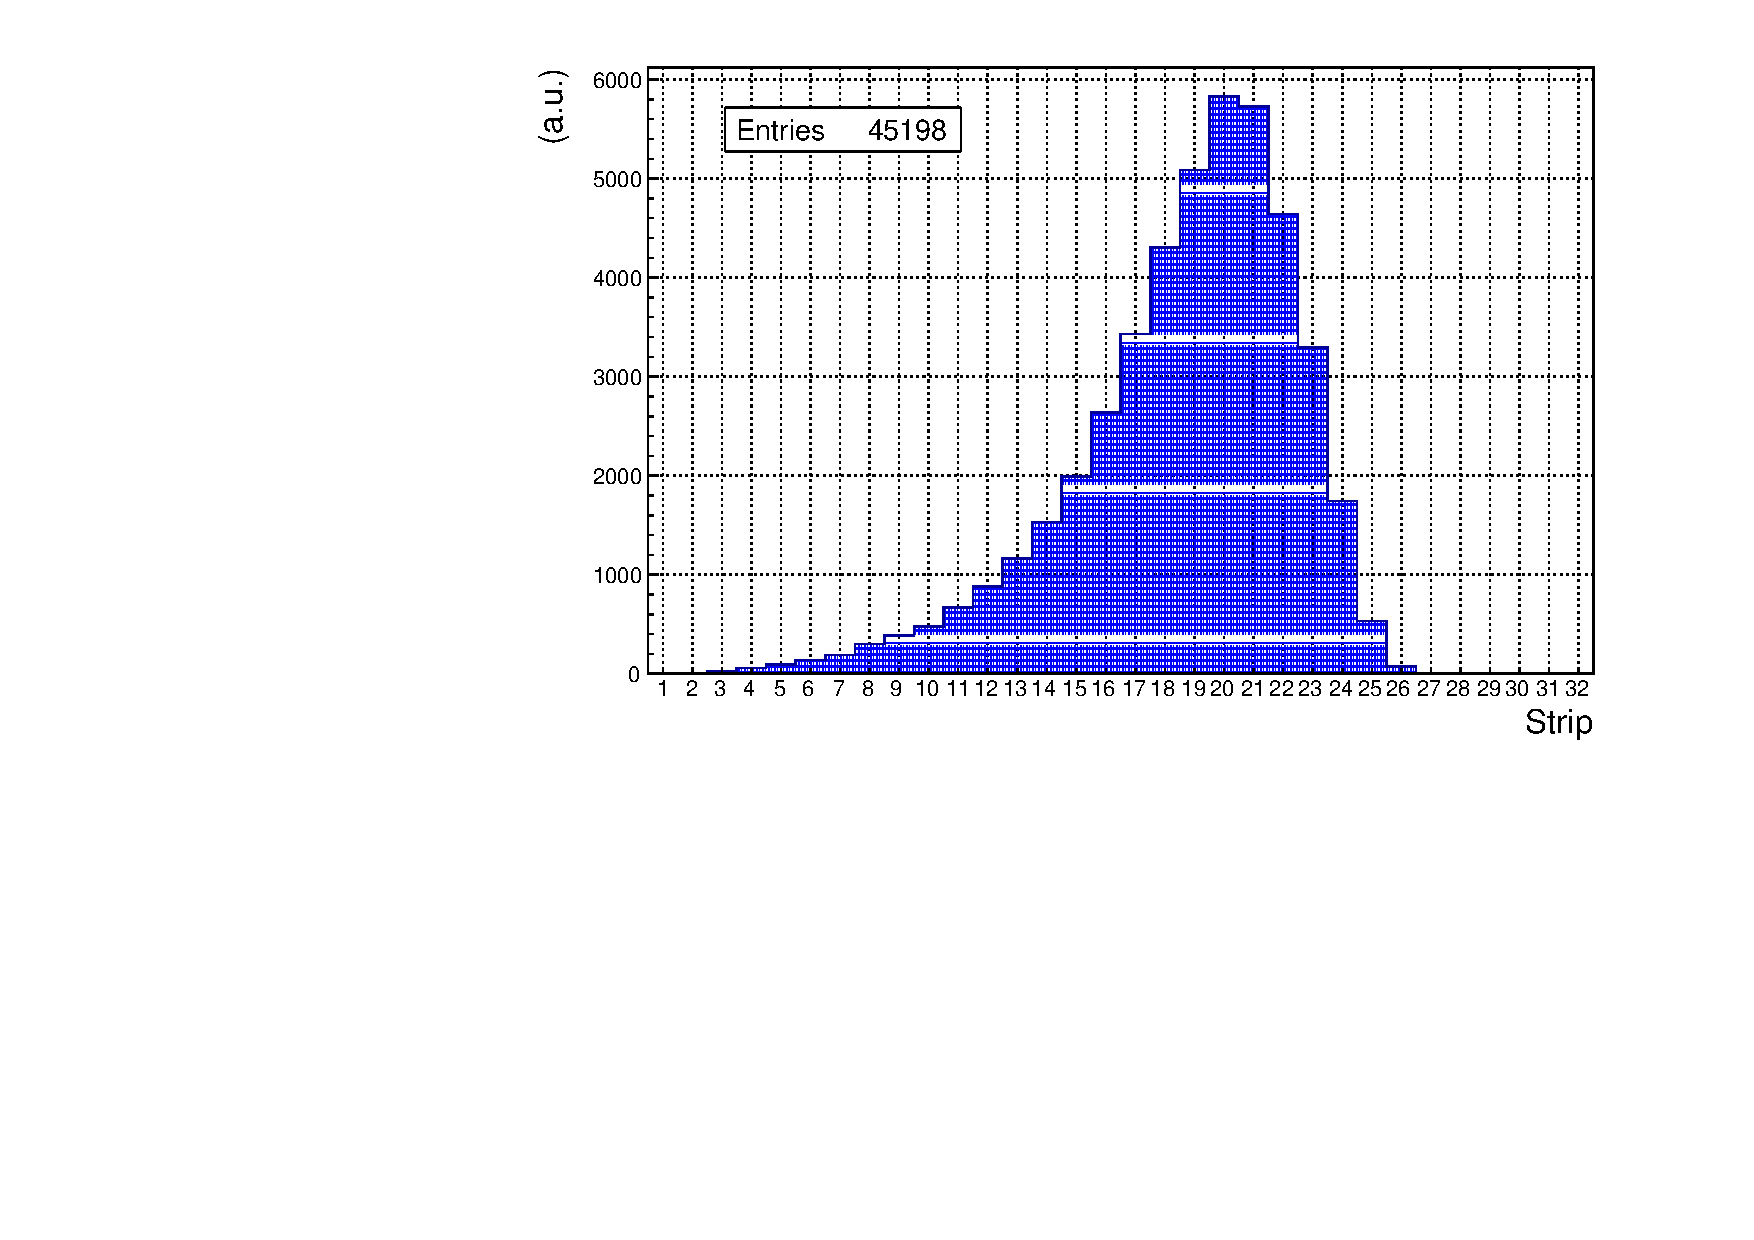
\includegraphics[width = \linewidth]{fig/chapt5/Geometrical-acceptance-forward.pdf}
			\caption{\label{fig:SimResult:B} Forward acceptance}
		\end{subfigure}
		\begin{subfigure}{\linewidth}
			\centering
			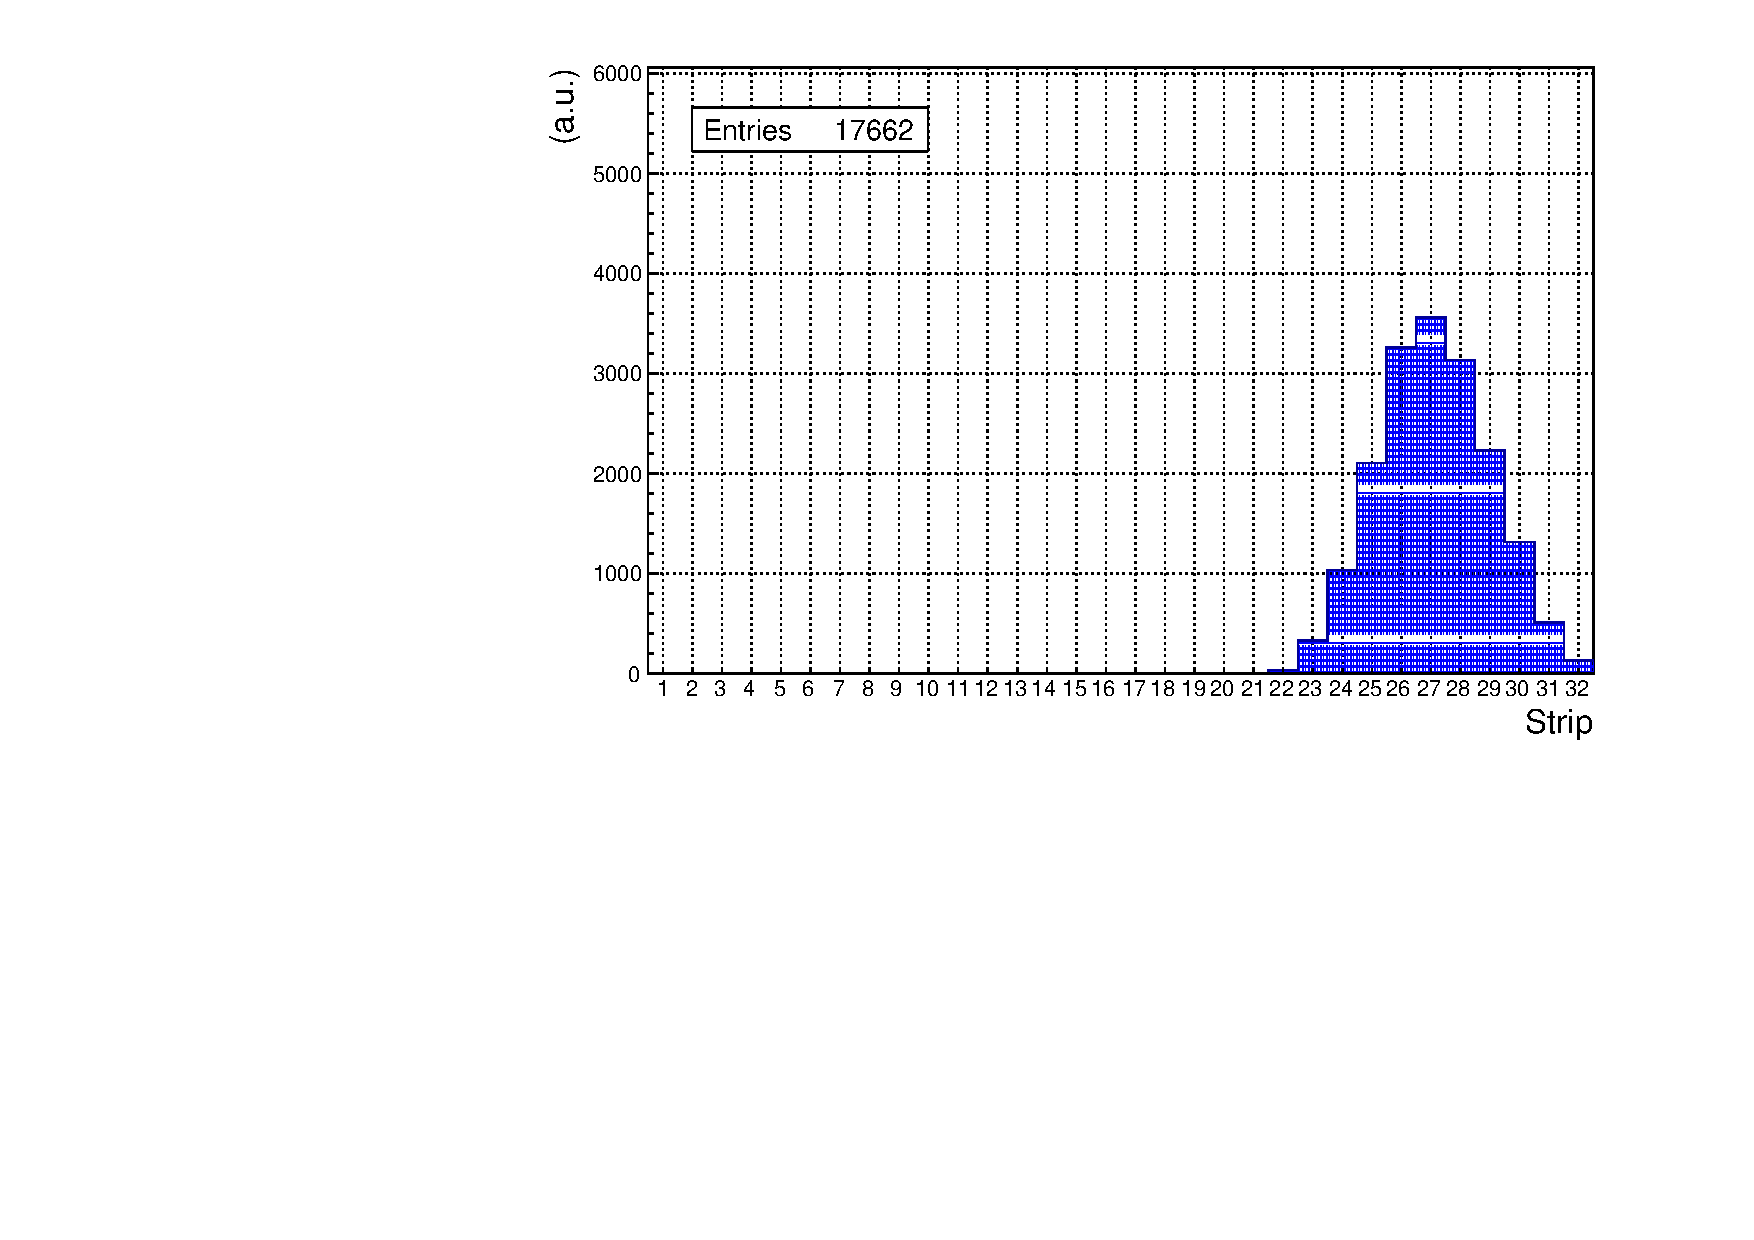
\includegraphics[width = \linewidth]{fig/chapt5/Geometrical-acceptance-backward.pdf}
			\caption{\label{fig:SimResult:C} Backward acceptance}
		\end{subfigure}
		\caption{\label{fig:SimResult} Geometrical acceptance distribution as provided by the \acl{MC} simulation.}
	\end{wrapfigure}
	
	The output from the simulation is given in Figure~\ref{fig:SimResult} in which the geometrical acceptance distribution of the setup is shown. The distributions for the separate contributions of forward coming and backward going muons are all provided. The strip number is given in a range of 1 to 32 corresponding to the 32 strips contained in each RPC read-out partition even though partition B correponds, by convention, to strip numbers 33 to 64. It can be established than, out of the total amount of muons that have passed through the telescope and reached the RPC, 16.8\% were hitting the 16 first strip of the read-out plane corresponding to half partition B1. This number correponds to the inefficiency. It can be used then to correct the data by scaling up by a factor $c_{geo} = 1/(1-0.168)$ the efficiency measured during data taking.
	
	Nevertheless, the distribution showed in Figure~\ref{fig:SimResult:A} differs from the measured hit profile showed in Figure~\ref{fig:HitProf} as can be seen in Figure~\ref{fig:Data-Acc-Comp}. It is difficult to evaluate a systematic uncertainty on this geometrical correction for different reasons.\\
	First of all, even though the dimensions of the scintillators and of the RPC are well known, the position of each element of the setup with respect to one another was not measured. The extraction of the position of each part of the setup from Figure~\ref{fig:GIF-RPCSetup} was a first large source of error.\\
	The inclination is also roughly measured to be \SI{10}{\degree} bringing more uncertainty into the simulation. The acceptance distribution would be affected by a variation of the inclination angle, as can be seen in Figure~\ref{fig:Acc-Angle}. Yet, the position of the acceptance peaks in the distribution would be in agreement with what is measured, and the contribution of farward and backward muons would never reach the observation. With an inclination of \SI{10}{\degree}, 28.1\% of the total geometrical acceptance should contribute to detecting backward muons whereas it is measured that the hit profile contains 22.0\% of backward data only. Introducing in the simulation an error of $\pm$\SI{2}{\degree} would lead to a correction factor $c_{geo} = 1.20^{+0.04}_{-0.03}$ allowing for a good improvement of the efficiency measured in GIF, as can be seen from Figure~\ref{fig:EffCorrection}. GIF measurement is in agreement with the reference curve within statistical errors.
	
\endgroup
\newpage

	\begin{figure}[H]
		\centering
		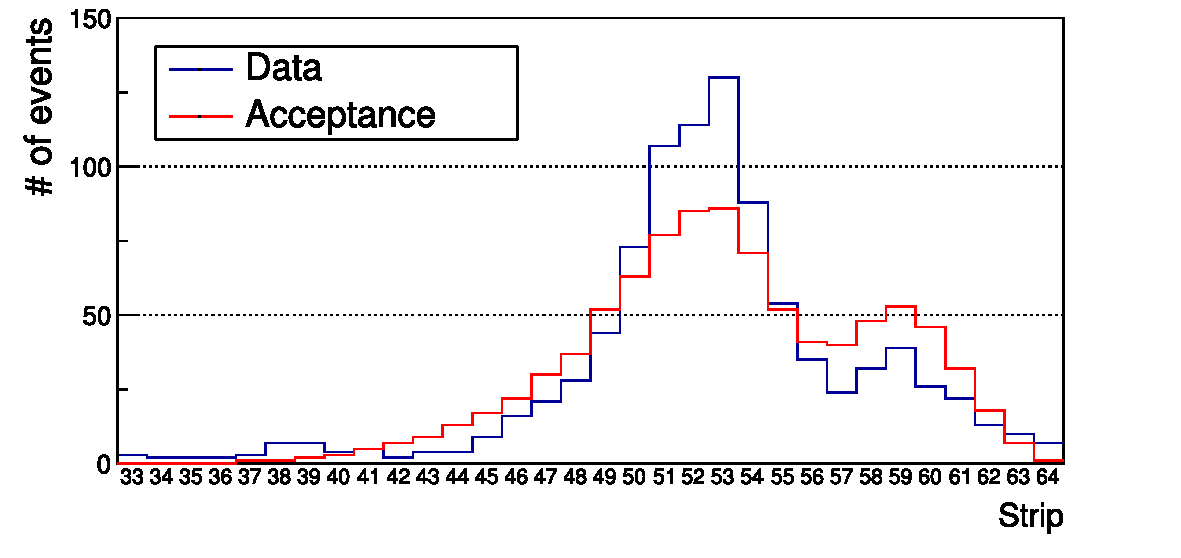
\includegraphics[width = .7\linewidth]{fig/chapt5/Data-Acc-Comp.pdf}
		\caption{\label{fig:Data-Acc-Comp} Comparison of the hit distribution recorded in the detector and of the normalised geometrical acceptance distribution.}
	\end{figure}

	\begin{figure}[H]
		\centering
		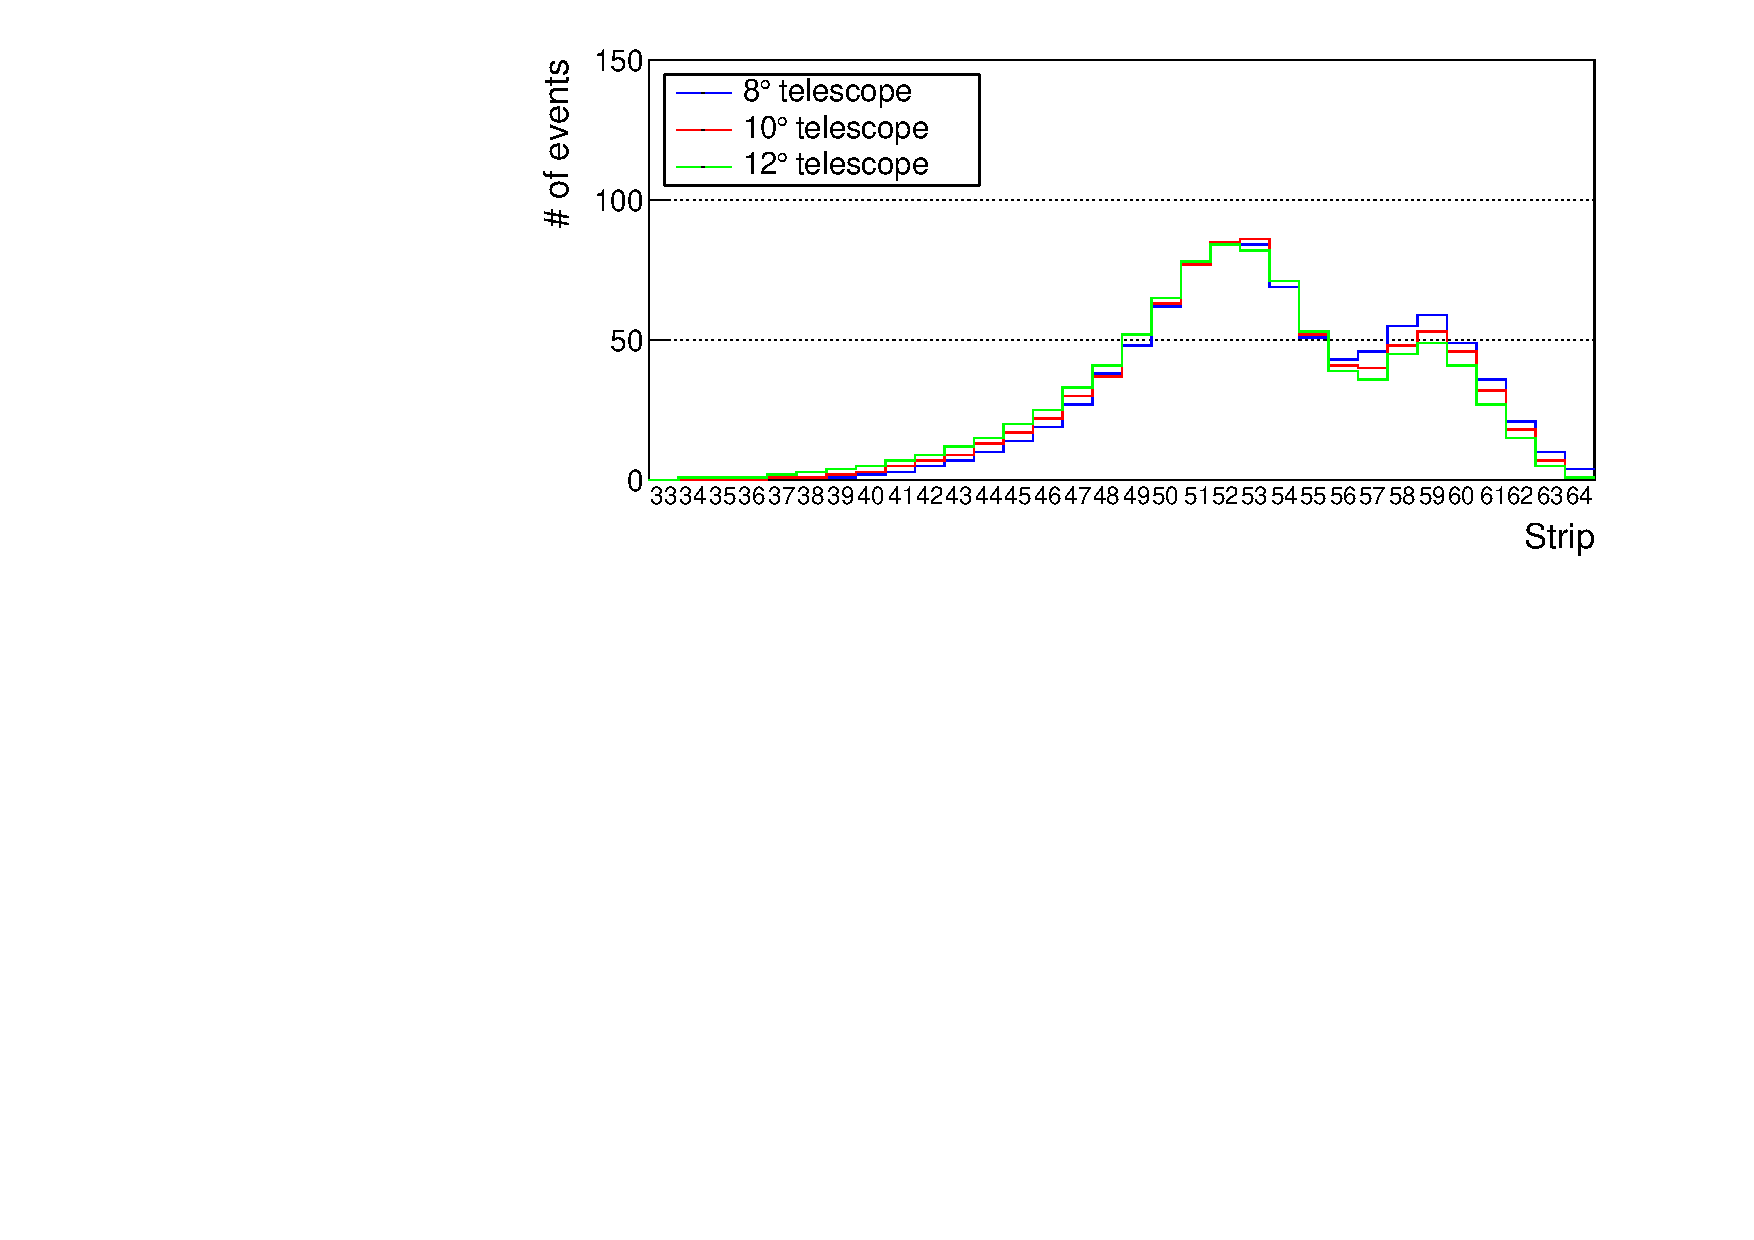
\includegraphics[width = .7\linewidth]{fig/chapt5/Acc-Angle.pdf}
		\caption{\label{fig:Acc-Angle} Effect of the variation of telescope inclination on the normalised geometrical acceptance distribution.}
	\end{figure}

	\begin{figure}[H]
		\centering
		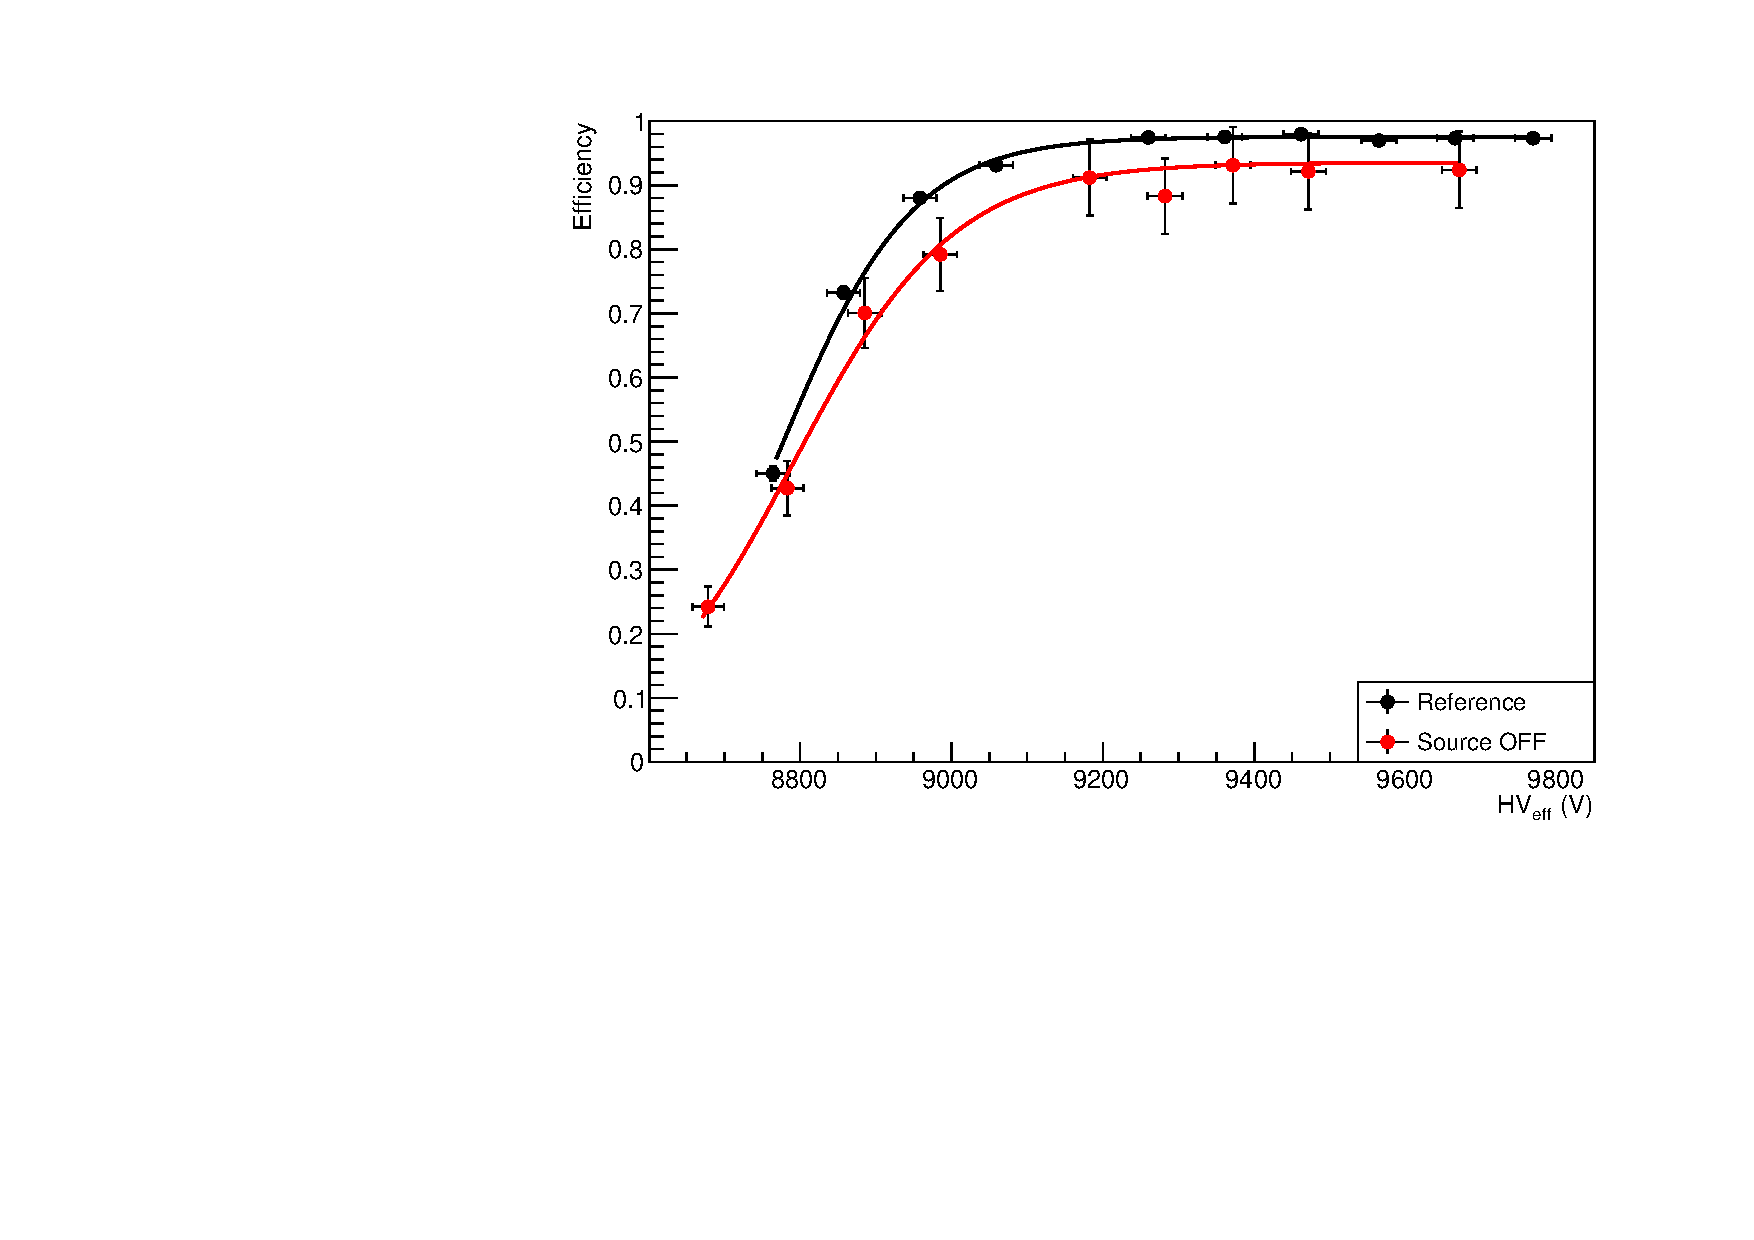
\includegraphics[width = .7\linewidth]{fig/chapt5/Compared-Efficiency-Correction.pdf}
		\caption{\label{fig:EffCorrection} Correction of the efficiency without source. The efficiency after correction gets much closer to the Reference measurement performed before the study in GIF by reaching a plateau of \numerror{93.52}{2.64}\%.}
	\end{figure}
	
\begingroup\setlength{\intextsep}{0pt}\setlength{\columnsep}{15pt}
	
	\begin{wrapfigure}{O}{.55\linewidth}
            \centering
		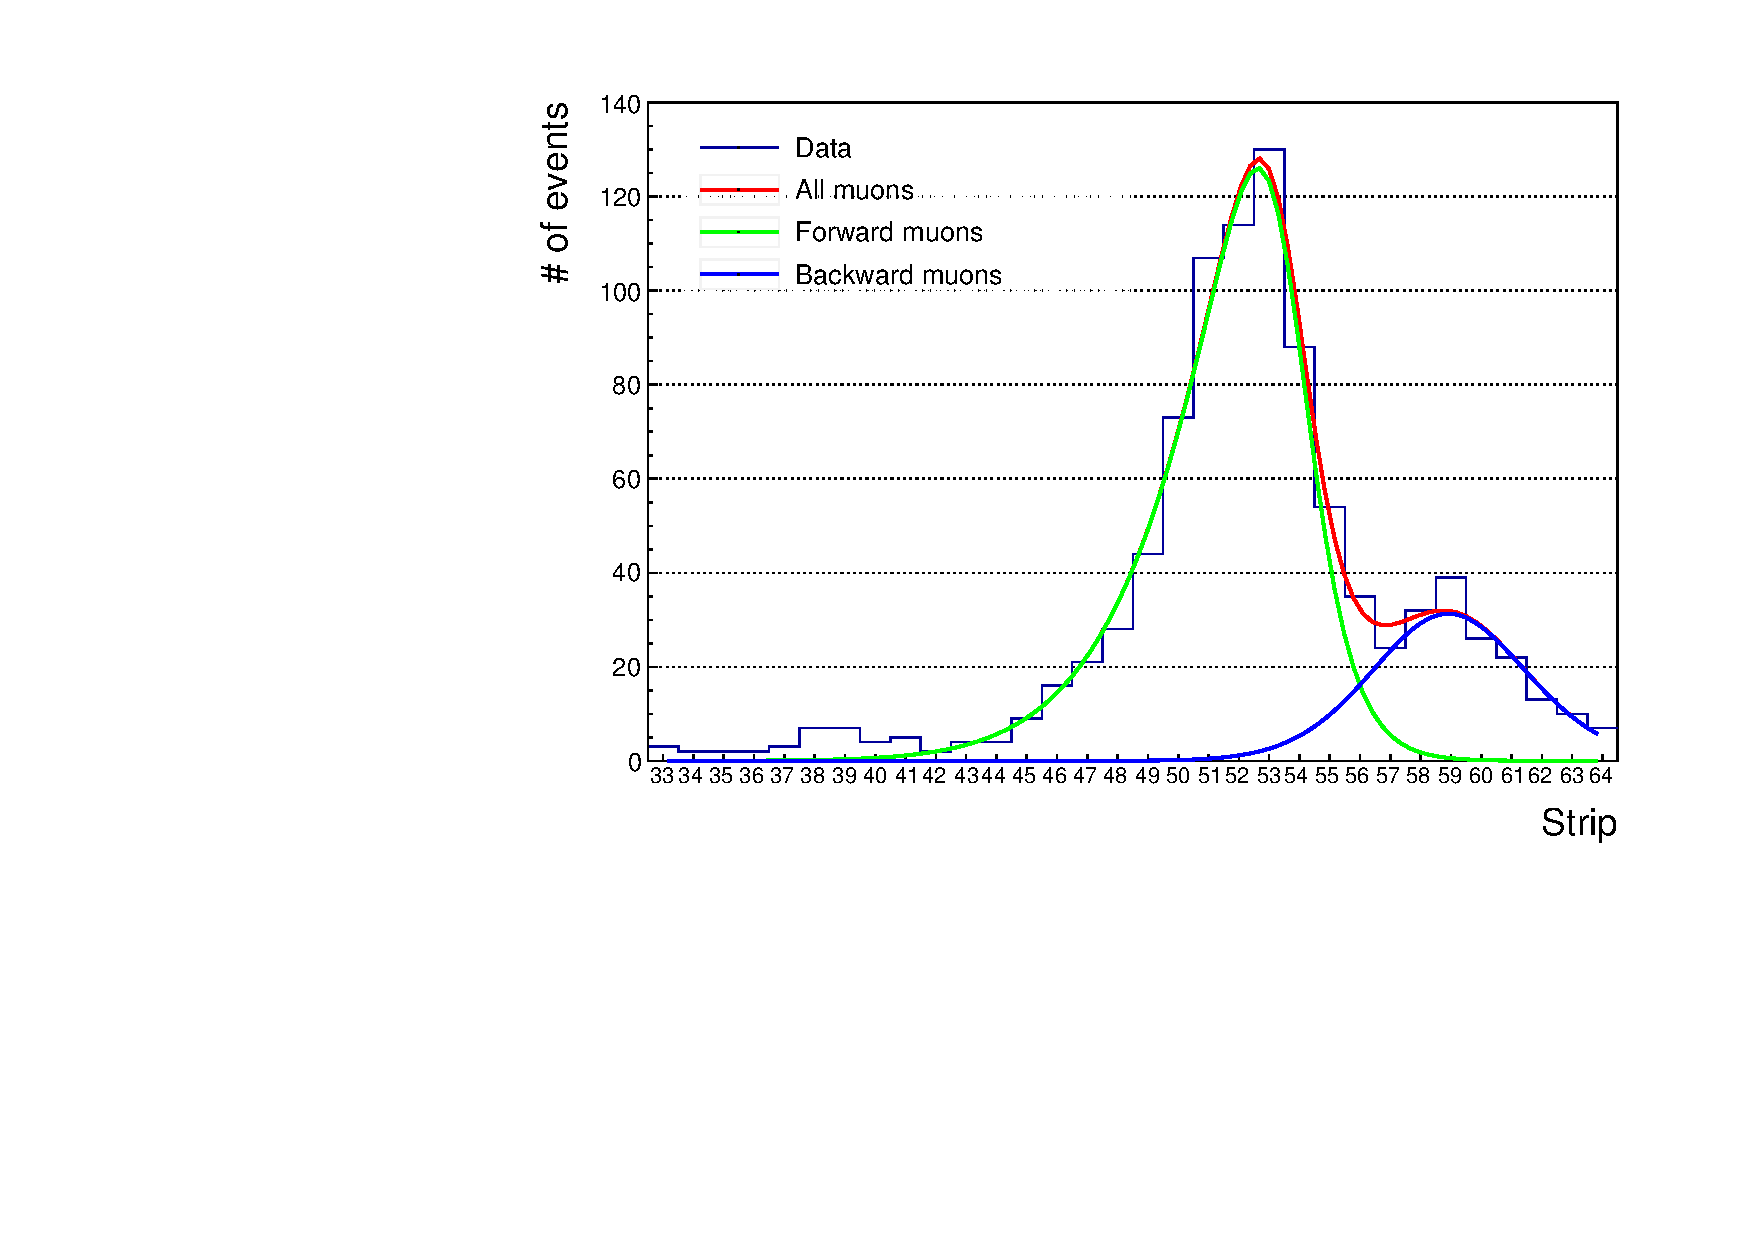
\includegraphics[width = \linewidth]{fig/chapt5/Cosmic-data-21-skew-fit.pdf}
		\caption{\label{fig:Fit-data} Hit distributions over read-out partition B of \texttt{RE-4-2-BARC-161} chamber together with skew distribution fits corresponding to forward and backward coming muons.}
	\end{wrapfigure}
	
	This estimation of the backward versus forward content in the data was done through a fit using a sum of two skew distributions given in Equation~\ref{eq:skew}. Although a skew distribution lacks physical interpretation, it allows fitting easily such kind of data, as showed in Figure~\ref{fig:Fit-data}.
	
	\begin{equation}
	\label{eq:skew}
		\begin{aligned}
	g(x) &= A_g e^{\frac{-(x-\bar{x})^2}{2\sigma^2}}\\
	s(x) &= \frac{A_s}{1+e^{-\lambda(x-x_i)}}\\
	sk(x) &= g(x)\times s(x)\\
	      &= A_{sk}\frac{e^{\frac{-(x-\bar{x})^2}{2\sigma^2}}}{1+e^{-\lambda(x-x_i)}}
		\end{aligned}
	\end{equation}

\endgroup
	
	Given the observed difference between the simulation and the measured data, one should realize that the geometrical acceptance and the hit profile are actually not directly comparable. The geometrical acceptance only provides with the information about what the detector can expect to see in a perfect world where all muons are detected in the exact same way. The detection would be independent from their energy or angle of incidence, and there would be no fluctuation of the detector gain due to complex avalanche development. No thresholds would be applied on the scintillators and on the RPC FEEs to reduce the noise, the cross-talk and the orresponding spread of the induced charge observed on the read-out strips. The hit profile provides the final product of all the previously mentioned contributions and can greatly differ from purely geometrical considerations. A full physics analysis involving softwares such as \texttt{GEANT} would be required to further refine the correction on the measured efficiency at GIF.
	
	\subsection{Photon flux at \acs{GIF}}
	\label{chapt5:ssec:gFlux}
		
	In order to understand and evaluate the $\gamma$ flux in the GIF area, simulations have been conducted at the time GIF was opened for research purposes~\cite{AGOSTEO1999}. Table~\ref{tab:Sim1997} gives the $\gamma$ flux for different distances $D$ to the source. The simulation was done using GEANT and a \acf{MCNP} transport code, and the flux $F$ is given with the estimated error from these packages expressed in \%.
	
	\begin{table}[H]
		\centering
		\begin{tabular}{|*{5}{c|}}
			\hline
			Nominal & \multicolumn{4}{c|}{Photon flux $F$ [\siflux]} \\
			\cline{2-5}
			ABS & at $D=$ \SI{50}{cm} & at $D=$ \SI{155}{cm} & at $D=$ \SI{300}{cm} & at $D=$ \SI{400}{cm} \\
			\hline
			1 & \Sci{0.12}{8} $\pm$ 0.2\% & \Sci{0.14}{7} $\pm$ 0.5\% & \Sci{0.45}{6} $\pm$ 0.5\% & \Sci{0.28}{6} $\pm$ 0.5\% \\
			\hline
			2 & \Sci{0.68}{7} $\pm$ 0.3\% & \Sci{0.80}{6} $\pm$ 0.8\% & \Sci{0.25}{6} $\pm$ 0.8\% & \Sci{0.16}{6} $\pm$ 0.6\% \\
			\hline
			5 & \Sci{0.31}{7} $\pm$ 0.4\% & \Sci{0.36}{6} $\pm$ 1.2\% & \Sci{0.11}{6} $\pm$ 1.2\% & \Sci{0.70}{5} $\pm$ 0.9\% \\
			\hline
		\end{tabular}
		\caption{\label{tab:Sim1997} Total photon flux ($E\gamma \leq$ \SI{662}{keV}) with statistical error predicted considering a $^{137}$Cs activity of \SI{740}{GBq} at different values of the distance $D$ to the source along the x-axis of irradiation field~\cite{AGOSTEO1999}.}
	\end{table}

\newpage
	
\begingroup\setlength{\intextsep}{5pt}\setlength{\columnsep}{15pt}
	
	\begin{wraptable}{O}{.65\linewidth}
		\centering
		\begin{tabular}{|*{4}{c|}}
			\hline
			Nominal & \multicolumn{3}{c|}{Correction factor $c$} \\
			ABS & at $D=$ \SI{155}{cm} & at $D=$ \SI{300}{cm} & at $D=$ \SI{400}{cm} \\
			\hline
			1 & $1.059 \pm 0.70\%$ & $1.162 \pm 0.70\%$ & $1.222 \pm 0.70\%$ \\
			\hline
			2 & $1.063 \pm 1.10\%$ & $1.150 \pm 1.10\%$ & $1.227 \pm 0.90\%$ \\
			\hline
			5 & $1.056 \pm 1.60\%$ & $1.130 \pm 1.60\%$ & $1.202 \pm 1.30\%$ \\
			\hline
		\end{tabular}
		\caption{\label{tab:CorrFactor} Correction factor c is computed with Formula~\ref{eq:Factor} taking as reference $D_0 =$ \SI{50}{cm} and the associated flux $F_0^{ABS}$ for each absorption factor available in table~\ref{tab:Sim1997}.}
	\end{wraptable}
	
	The table however does not provide in a direct way the flux at the level of the RPC under test. First of all, it is necessary to extract the value of the flux from the available data contained in the original paper and then to estimate the flux in 2014 at the time the experimentation took place. The extraction will be performed for the case of a pointlike source emitting isotrope and homogeneous gamma radiations. The flux $F_0$ is known at a given reference point situated at $D_0$ from the source. The gamma flux $F$ at a distance $D$ from the source will be expressed with Equation~\ref{eq:Flux}, assuming that the flux decreases as $1/D^2$ and where $c$ is a fitting factor that can be written as in Equation~\ref{eq:Factor}. Finally, using Equation~\ref{eq:Factor} and the data of Table~\ref{tab:Sim1997}, with $D_0=$ \SI{50}{cm} as reference point, Table~\ref{tab:CorrFactor} can be built. It is interesting to note that $c$ for each value of $D$ does not depend on the absorption factor.

\endgroup
	
	\begin{minipage}{.49\linewidth}
	\begin{equation}
	\label{eq:Flux}
	F^{ABS} = F_0^{ABS} \times \left( \frac{c D_0}{D} \right)^2
	\end{equation}
	\end{minipage}
	\hfill
	\begin{minipage}{.49\linewidth}
	\begin{equation}
	\label{eq:Factor}
		\begin{aligned}
		c &= \frac{D}{D_0}\sqrt{\frac{F^{ABS}}{F_0^{ABS}}}\\
		\Delta c &= \frac{c}{2}\left(\frac{\Delta F^{ABS}}{F^{ABS}}+\frac{\Delta F^{ABS}_0}{F^{ABS}_0}\right)
		\end{aligned}
	\end{equation}
	\end{minipage}
	\vspace{5mm}
	
	For the range of $D/D_0$ values available, it is possible to use a simple linear fit to get the evolution of $c$ that can be expressed as $c(D/D_0)=aD/D_0+b$. Using Formula~\ref{eq:FluxLinearAp}, but neglecting the uncertainty on $D$ that will only be used when extrapolating the values for the position of the RPC under test whose position is not perfectly known, the results shown in Figure~\ref{fig:CorrFactor} is obtained. Figure~\ref{fig:CorrFactor:B} confirms that using only a linear fit to extract $c$ is enough as the evolution of the rate that can be obtained superimposes well on the simulation points.
	
	\begin{equation}
	\label{eq:FluxLinearAp}
	F^{ABS} = F^{ABS}_0 \left( a + \frac{bD_0}{D} \right)^2 \; , \quad \Delta F^{ABS} = F^{ABS} \left[\frac{\Delta F^{ABS}_0}{F^{ABS}_0} + 2\frac{\Delta a + \Delta b\frac{D_0}{D} + \Delta D\frac{bD_0}{D^2}}{a + \frac{bD_0}{D}}\right]
	\end{equation}
	
	During the 2014 GIF tests, the RPC read-out plane was located at a distance $D=$ \SI{206}{cm} from the source. Moreover, to estimate the strength of the flux in 2014, it is necessary to consider the nuclear decay through time of the Cesium source whose half-life is well known ($t_{1/2}=$ \SIerror{30.05}{0.08}{y}). The very first source activity measurement has been done on the \Th{5} of March 1997 while the GIF tests where done in between the \Th{20} and the \Th{31} of August 2014, i.e. at a time $t=$ \SIerror{17.47}{0.02}{y} resulting in an attenuation of the activity from \SI{740}{GBq} in 1997 to \SI{494}{GBq} in 2014. All the needed information to extrapolate the expected flux through the detector at the moment of the GIF preliminary tests has now been assembled, leading to Table~\ref{tab:extra2014}. By assuming an average sensitivity of the RPC to $\gamma$ emitted by the $^{137}$Cs source of \SciErr{2}{0.2}{-3}~\cite{PUGLIESE2003}, the order of magnitude of the expected hit rate per unit area would be of the order of \si{kHz} for a fully opened source, as reported in the last column of the table. As photons are not charged particles, they mainly interact with the electrodes where they are converted into electrons. The HPL electrodes are not very sensitive to gamma photons, hence only a small fraction of the incoming flux is seen by the RPC.
	
	\begin{figure}[H]
		\begin{subfigure}{\linewidth}
			\centering
			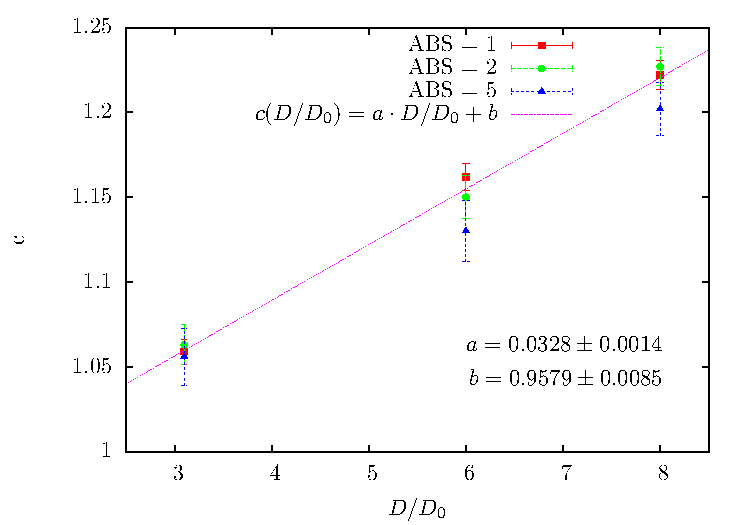
\includegraphics[width = .6\linewidth]{fig/chapt5/flux_correction.pdf}\\
			\caption{\label{fig:CorrFactor:A}}
		\end{subfigure}
		\begin{subfigure}{\linewidth}
			\centering
			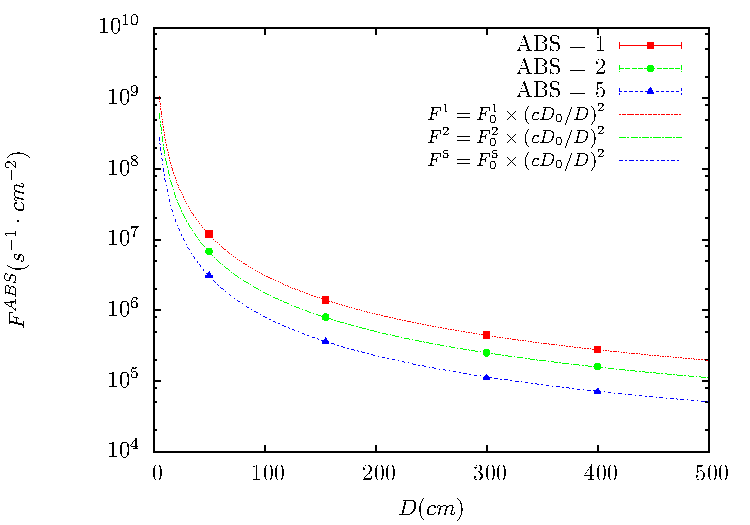
\includegraphics[width = .6\linewidth]{fig/chapt5/correction_model.pdf}
			\caption{\label{fig:CorrFactor:B}}
		\end{subfigure}
		\caption{\label{fig:CorrFactor} \subref{fig:CorrFactor:A} Linear approximation fit performed on the data extracted from table~\ref{tab:CorrFactor}. \subref{fig:CorrFactor:B} Comparison of Equation~\ref{eq:FluxLinearAp} with the simulated flux using $a$ and $b$ given in figure~\ref{fig:CorrFactor:A} in Equation~\ref{eq:Flux} and the reference $D_0 =$ \SI{50}{cm} and the associated flux for each absorption factor $F_0^{ABS}$ from table~\ref{tab:Sim1997}.}
	\end{figure}
	
	\begin{table}[H]
		\begin{tabular}{|*{5}{c|}}
			\hline
			Nominal & \multicolumn{3}{c|}{Photon flux $F$ [\siflux]} & Rate [\sirate] \\
			ABS & at $D_0^{97}=$ \SI{50}{cm} & at $D^{97}=$ \SI{206}{cm} & at $D^{2014}=$ \SI{206}{cm} & at $D^{2014}=$ \SI{206}{cm} \\
			\hline
			1 & \Sci{0.12}{8} $\pm$ 0.2\% & \Sci{0.84}{6} $\pm$ 1.2\% & \Sci{0.56}{6} $\pm$ 1.2\% & $1129 \pm 14$ \\
			\hline
			2 & \Sci{0.68}{7} $\pm$ 0.3\% & \Sci{0.48}{6} $\pm$ 1.2\% & \Sci{0.32}{6} $\pm$ 1.2\% & $640 \pm 8$ \\
			\hline
			5 & \Sci{0.31}{7} $\pm$ 0.4\% & \Sci{0.22}{6} $\pm$ 1.2\% & \Sci{0.15}{6} $\pm$ 1.2\% & $292 \pm 4$ \\
			\hline
		\end{tabular}
		\caption{\label{tab:extra2014} The data at $D_0$ in 1997 is taken from~\cite{AGOSTEO1999}. Using Formula~\ref{eq:FluxLinearAp}, the flux at $D$, including an error of \SI{1}{cm}, can be estimated in 1997. Then, taking into account the attenuation of the source activity, the flux at $D$ can be estimated at the time of the tests in GIF in 2014. Assuming a sensitivity of the RPC to gammas, $s =$ \SciErr{2}{0.2}{-3}~\cite{PUGLIESE2003}, an estimation of the hit rate per unit area is obtained.}
	\end{table}
	
	The goal of the study was to have a good measurement of the intrinsic RPC performance without source irradiation. Then, taking profit of the two working absorbers, at absorption factors 5 (\SI{300}{Hz}) and 2 ($\sim$\SI{600}{Hz}) the goal was to show that the detectors fulfill the performance certification of CMS RPCs. Finally, a first assessment of the performance of the detectors at higher backgrounds was obtained with absorbtion factor 1 (no absorption and $>$\SI{1}{kHz})).
	
	\subsection{Results and discussions}
	\label{chapt5:ssec:resultsGIF}
	
	The data taking at GIF has been conducted between the \St{21} and the \St{31} of August, 2014. Data have been collected with source both ON and OFF using three different absorber settings (ABS 5, 2 and 1) in order to vary the irradiation on the RPC. For each source setting, two HV scans have been performed with two different trigger settings. During a first scan the trigger sent to the TDC module was the coincidence of the two scintillators composing the telescope while during a second scan the trigger was a pulse coming from a pulse generator in order to measure the noise or gamma rate seen by the chamber. Indeed, using a pulse generator allows to trigger at moments not linked to any physical event and, hence, to obtain a \textit{RANDOM} trigger on noise and gamma events to measure the associated rates, the probability to have a pulse in coincidence with a cosmic muon being negligible.
	
	From the cosmic trigger scans, a summary of the efficiencies and corresponding cluster sizes is shown in Figure~\ref{fig:GIFEffCS}. The efficiency curves with Source ON show a shift with respect to the case without irradiation. With ABS 5, the general shape of the efficiency curve stays unchanged whereas a clear alteration of the performance is observed at ABS 2 and ABS 1. From the cluster size results, a reduction of the mean cluster size under irradiation can be observed at equivalent efficiency. This effect can be due to the perturbation of the electric field by the strong flux of gamma particles interacting with the electrodes. With the increasing number of photons being converted into electrons, an increasing number of charges need to be recombined all over the volume of the electrodes that act as capacitors. A discharge of the electrodes reduces the effective field seen in the gas volume by introducing a voltage drop across the electrodes thickness. The constant pressure put on the detector by the converting photons can become strong enough to uniformly affect the gain of the detector.
	
	\begin{figure}[H]
    	\begin{subfigure}{.5\linewidth}
			\centering
			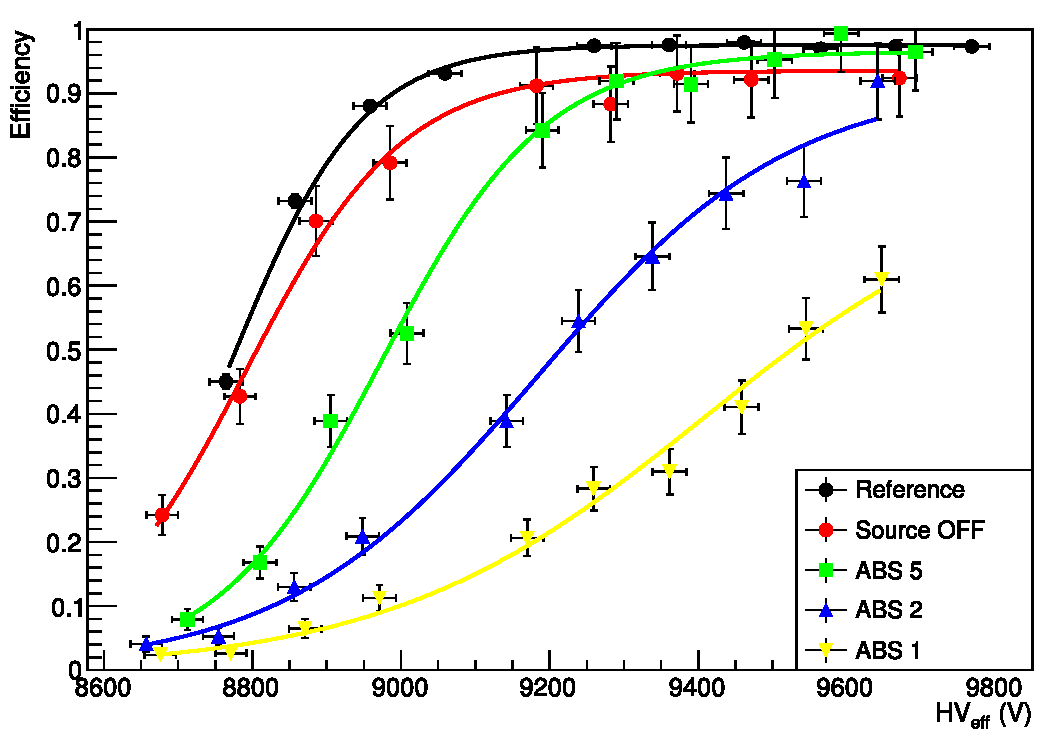
\includegraphics[width = \linewidth]{fig/chapt5/Efficiency.pdf}
        	\caption{\label{fig:GIFEffCS:A}}
    	\end{subfigure}
    	\begin{subfigure}{.5\linewidth}
			\centering
			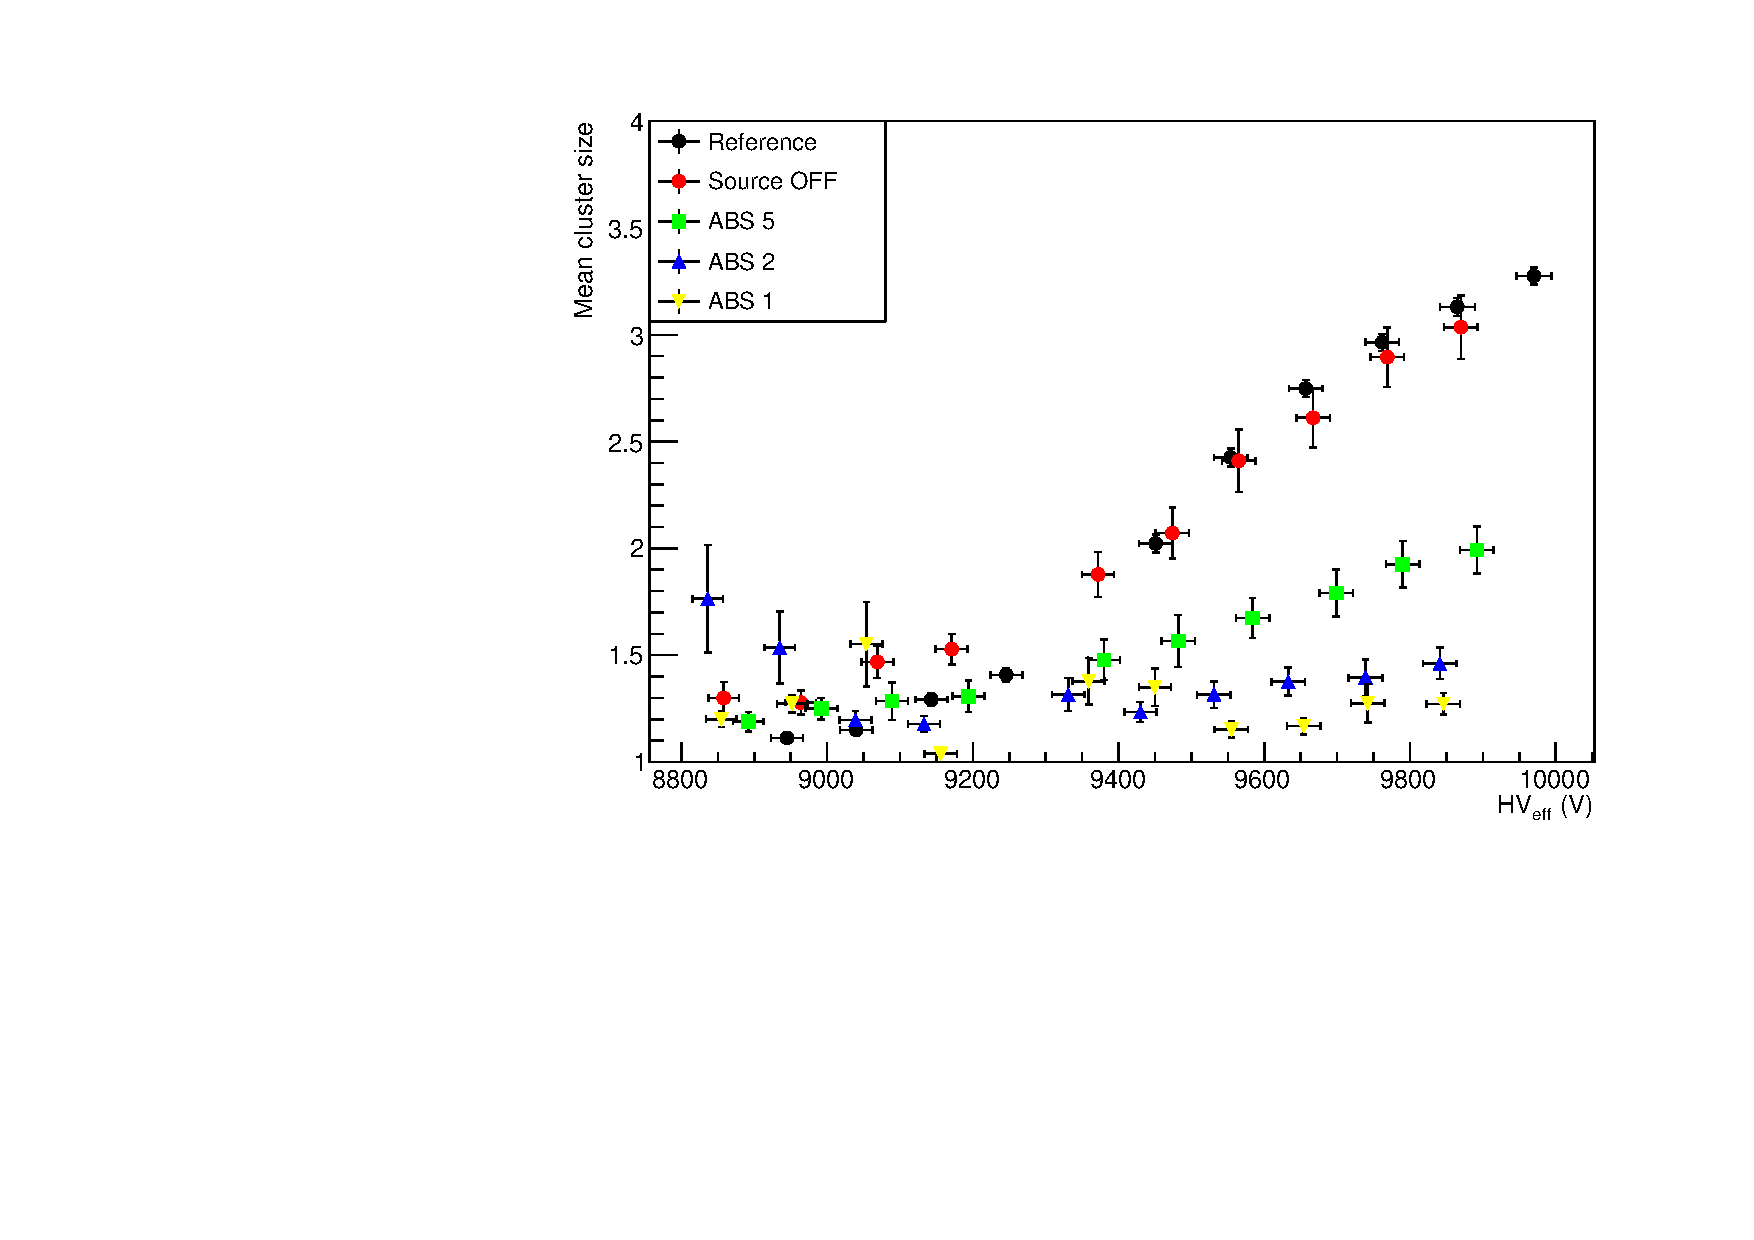
\includegraphics[width = \linewidth]{fig/chapt5/Cluster-Size.pdf}
        	\caption{\label{fig:GIFEffCS:B}}
    	\end{subfigure}
		\caption{\label{fig:GIFEffCS} Efficiency~\subref{fig:GIFEffCS:A} and cluster size~\subref{fig:GIFEffCS:B} of chamber \texttt{RE-4-2-BARC-161} measured at GIF with Source OFF (red) and Source ON using different absorber settings: ABS 5 (green), ABS 2 (blue) and ABS 1 (yellow). The results are compared to the Reference values obtained with cosmics.}
	\end{figure}
	
	It is necessary to study the evolution of the performance of the chamber with the increasing rate per unit area. The hit rate is measured as the number of hits detected in the RPC normalized to the surface area of the read-out and to the total integrated time. The integrated time is linked to the time window in which the TDC searches for data related to a trigger signal. Data is continuously kept in the buffer of the TDCs but not all of these data is of interest. When a trigger signal is sent to the TDC module, the TDC saves all of the data located in a certain time window set around the time stamp of the signal. The total integrated time is then the total number of trigger signals times the width of a search time window.\\
	In Figure~\ref{fig:GIFRate:A}, the noise rate when the source is OFF remains low but increases at voltages above \SI{9500}{V}. Aside of the natural increase of the noise with increasing voltage, the rise of the noise rate in the detector can be related to the increased streamer probability observed with such a large electric field. The rates measured at GIF with source ON all show a similar behaviour until a high voltage of approximately \SI{9400}{V} at which the rate of ABS 5 reaches a plateau, coinciding with the chamber reaching full efficiency. It is important to note that, even though the rates look similar independently from the gamma flux, relative to the efficiency of the chamber, the rate actually increases with increasing flux at equivalent efficiency. A rough way to measure the rate effectively observed by the detector for each source setting would be to normalize the measured rates to the efficiency of the detector. This exercise was done with Figure~\ref{fig:GIFRate:B} from which constant fits where done on Source ON data in order to extract the rate the chamber was subjected to. This method leads to rates of \SIerror{164}{12}{Hz/cm^2}, \SIerror{340}{26}{Hz/cm^2} and \SIerror{598}{50}{Hz/cm^2} respectively for ABS 5, 2 and 1 which is consistent with the absorber values. Also, contrary to the case of the source OFF measurement, no rise of the noise is observed at ABS 5. This difference could be explained by the efficiency shift that is related to a decrease of the electric field across the gas volume. \textbf{[But, as no data were taken at higher voltage values, this assumption can't be confirmed.]} \textit{Could be confirmed by a study of the streamer probability for each dataset.}
	
	\begin{figure}[H]
    	\begin{subfigure}{.5\linewidth}
			\centering
			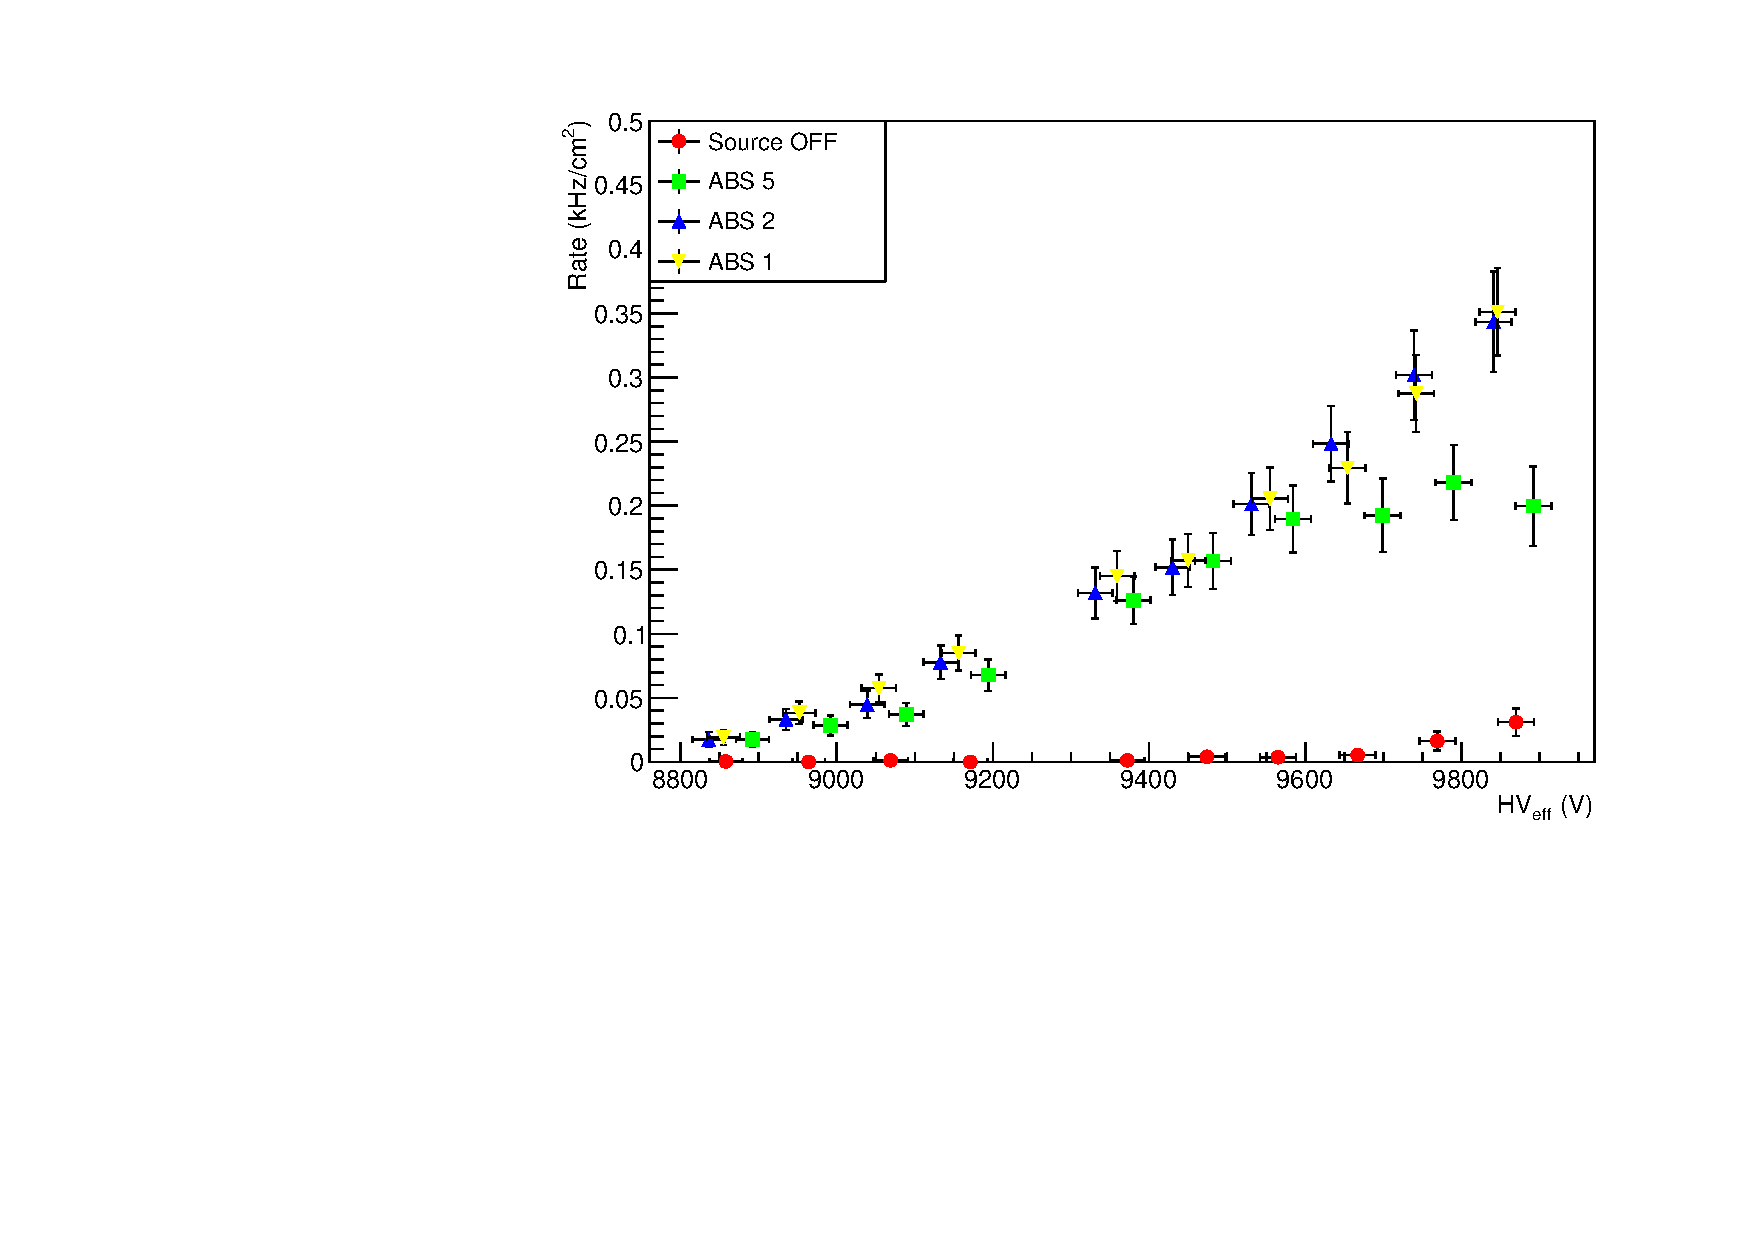
\includegraphics[width = \linewidth]{fig/chapt5/Gamma-Rate.pdf}
        	\caption{\label{fig:GIFRate:A}}
    	\end{subfigure}
    	\begin{subfigure}{.5\linewidth}
			\centering
			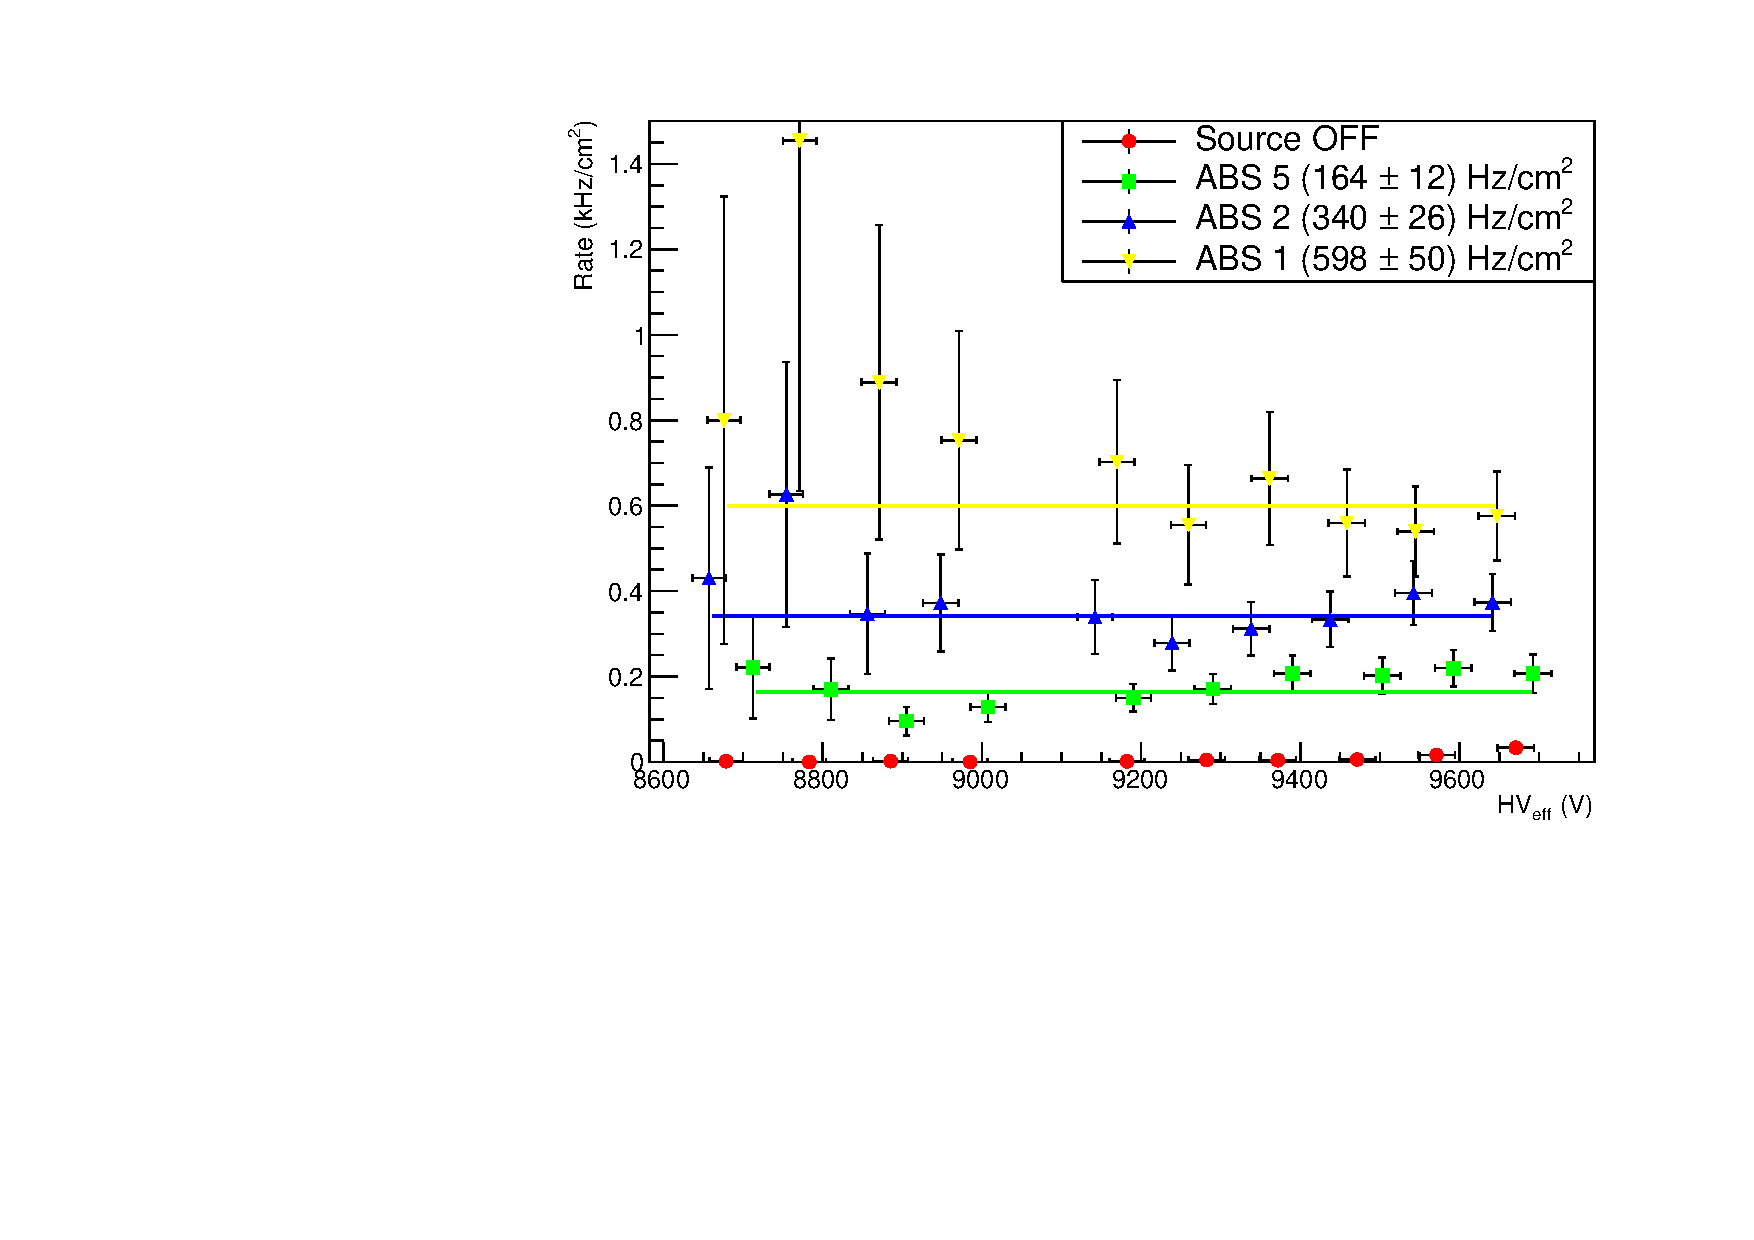
\includegraphics[width = \linewidth]{fig/chapt5/Unconvoluted-Gamma-Rate.pdf}
        	\caption{\label{fig:GIFRate:B}}
    	\end{subfigure}
		\caption{\label{fig:GIFRate} Rates in chamber \texttt{RE-4-2-BARC-161} measured at GIF with Source OFF (red) and Source ON using different absorber settings: ABS 5 (green), ABS 2 (blue) and ABS 1 (yellow). On Figure~\subref{fig:GIFRate:B}, the rates of Figure~\subref{fig:GIFRate:A} were normalized to the measured efficiency, and constant fits are performed on Source ON data showing the gamma rate in the chamber.}
	\end{figure}
	
	The results need to be taken with care as a better estimation of the rate would have been to push the detector towards higher voltages to reach the efficiency plateau for each absorber configuration and only then extract the measured rate at working voltage, defined as in Formula~\ref{eq:KneeWP}. Nevertheless, using this method to estimate the rate to which the chamber is subjected, it is possible to look at the evolution of the $HV_{50}$ and $HV_{knee}$ as a function of the increasing rate as showed in Figure~\ref{fig:Evolution}. The results from GIF suggest that at a rate of \SIrate{600} the working voltage of the chamber is increased by a thousand \si{V} while the efficiency is reduced to approximately 80\%, although the result still is consistent with an efficiency better than 90\% due to the large error on the measurement.
	
	\begin{figure}[H]
    	\begin{subfigure}{0.5\linewidth}
			\centering
    		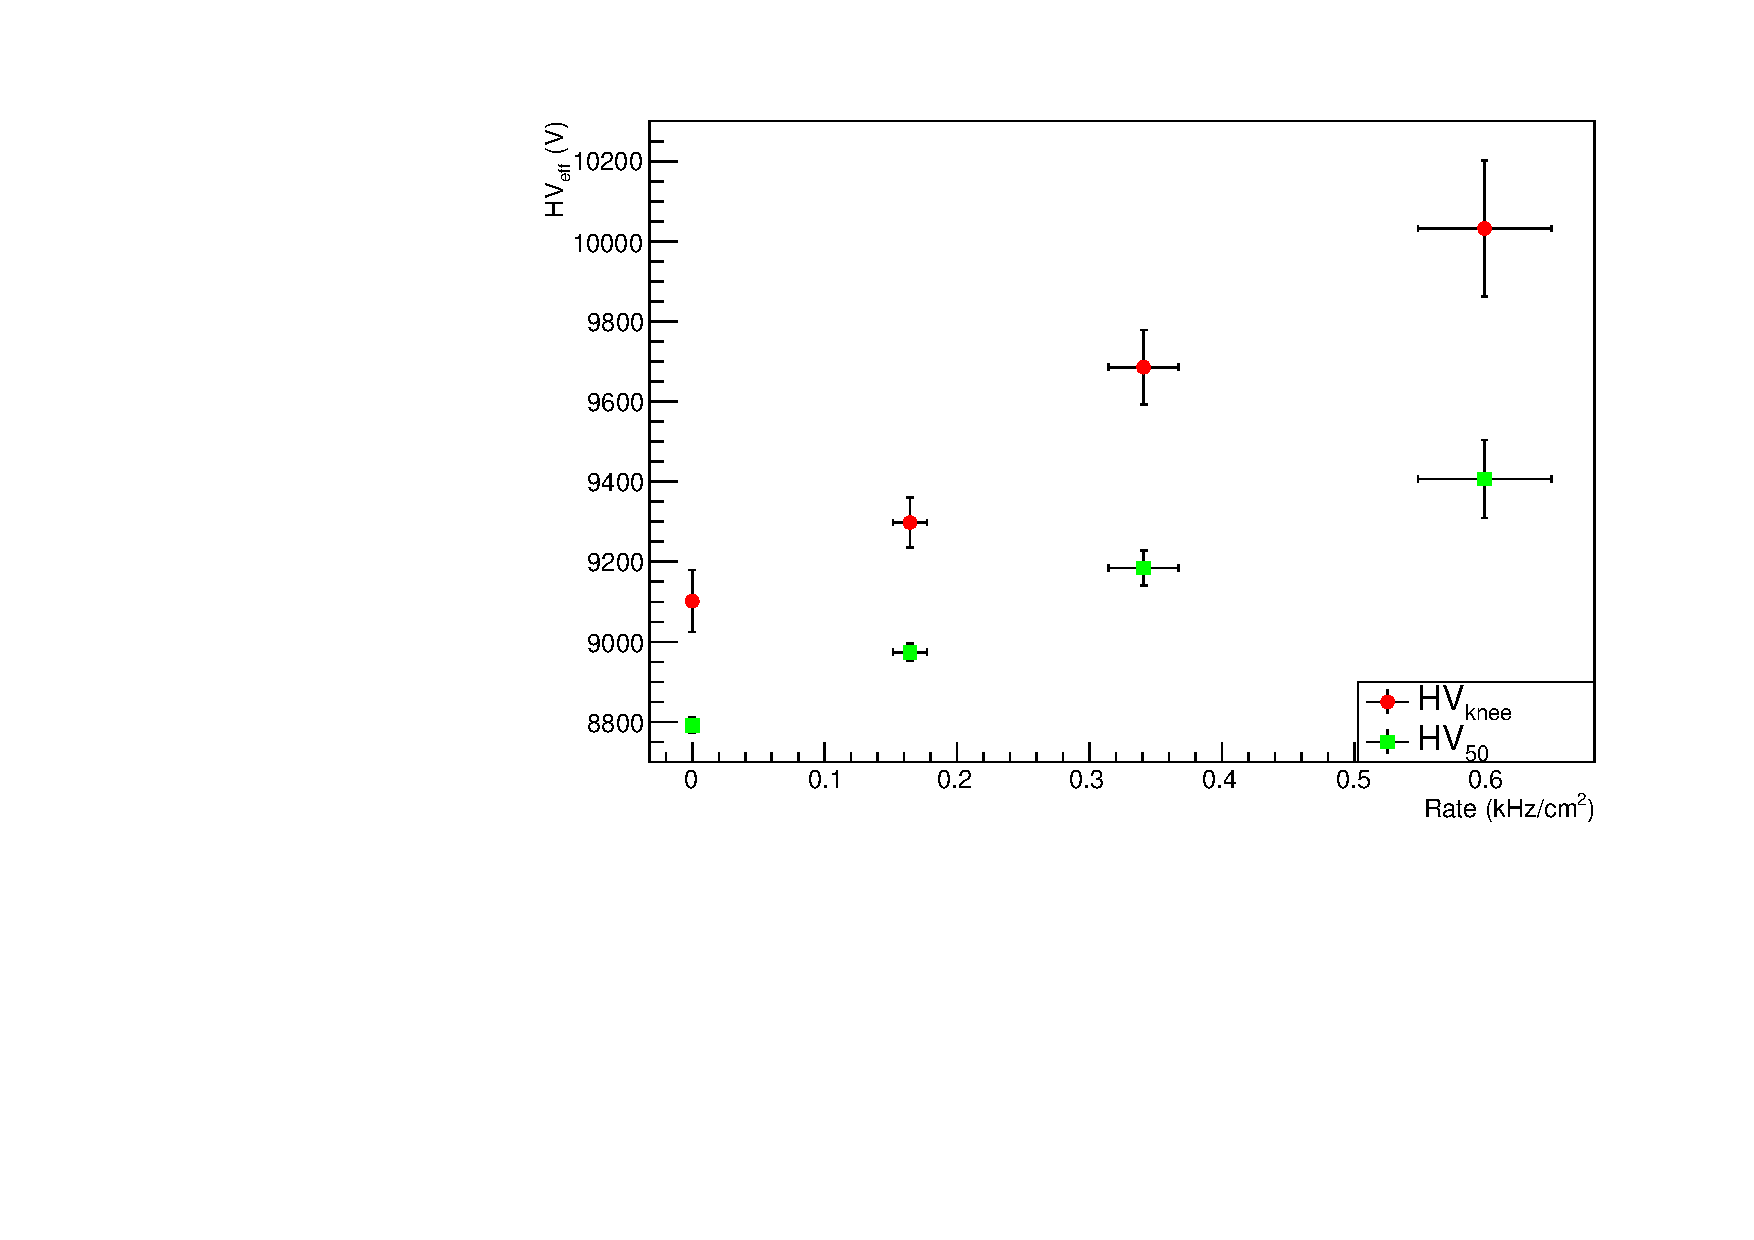
\includegraphics[width = 0.7\plotwidth]{fig/chapt5/HV-Knee-ABS.pdf}
        	\caption{\label{fig:Evolution:A}}
    	\end{subfigure}
    	\begin{subfigure}{0.5\linewidth}
			\centering
    		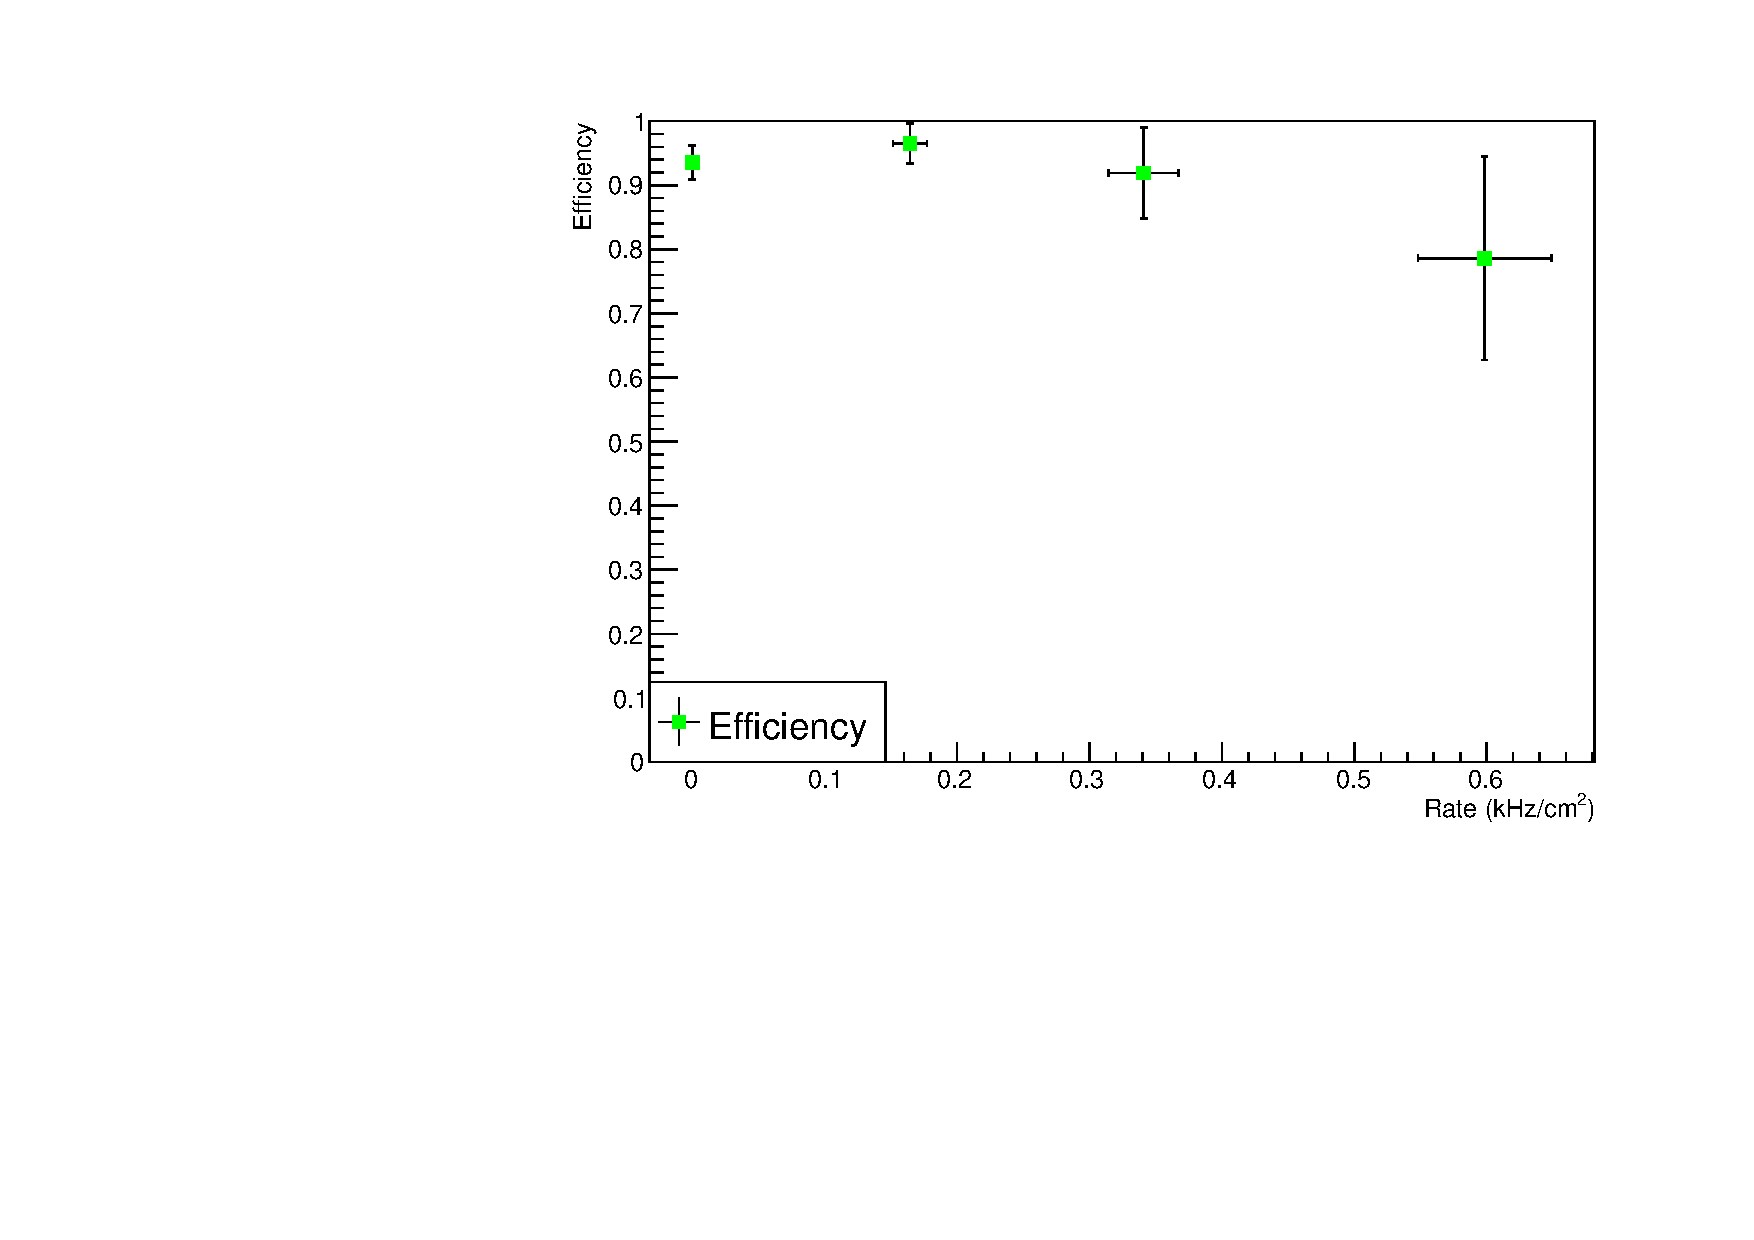
\includegraphics[width = 0.7\plotwidth]{fig/chapt5/Eff-ABS.pdf}\\
        	\caption{\label{fig:Evolution:B}}
    	\end{subfigure}
		\caption{\label{fig:Evolution} Evolution of the voltages at half maximum and at 95\% of the maximum efficiency (Figure~\ref{fig:Evolution:A}), and of the maximum efficiency (Figure~\ref{fig:Evolution:B}) as a function of the rate in chamber \texttt{RE-4-2-BARC-161}. The data is extracted from the fits in Figures~\ref{fig:GIFEffCS:A} and~\ref{fig:GIFRate:B}.}
	\end{figure}
	
	\begin{figure}[H]
    	\begin{subfigure}{0.69\linewidth}
			\centering
    		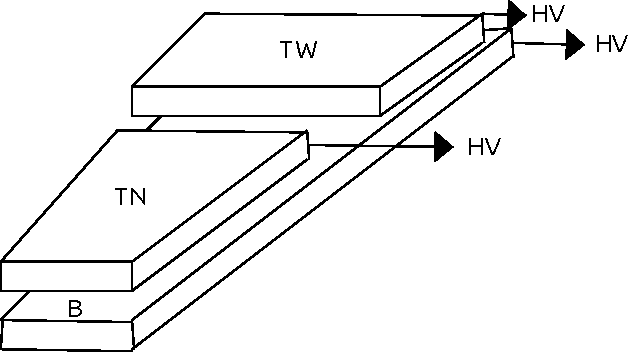
\includegraphics[height = 5cm]{fig/chapt5/Endcap-3D.pdf}
        	\caption{\label{fig:EndcapRPC:A}}
    	\end{subfigure}
    	\begin{subfigure}{0.29\linewidth}
			\centering
    		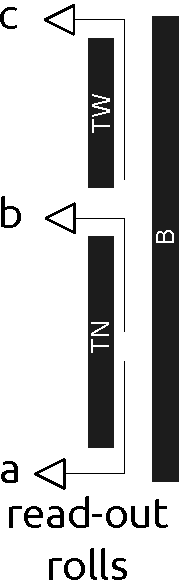
\includegraphics[height = 5cm]{fig/chapt5/Endcap-side.pdf}\\
        	\caption{\label{fig:EndcapRPC:B}}
    	\end{subfigure}
		\caption{\label{fig:EndcapRPC} Presentation of a double-gap endcap RPC with its three RPC gaps. Due to the partitioniing of the read-out strips into three rolls, the TOP layer of gap is divided into two gaps: TOP NARROW (TN) and TOP WIDE (TW). The BOTTOM (B) only consists in one gap.}
	\end{figure}
	
	It is likely that the rates obtained through fitting on normalized values is underestimated. Indeed, monitoring the current in the three gaps composing a CMS endcap RPC (Figure~\ref{fig:EndcapRPC}) while knowing the rate, the charge deposition per avalanche $q_\gamma$ can be computed. A current density, expressed in \si{A/cm^2}, divided by a rate per unit area, expressed in \si{Hz/cm^2} yields a charge expressed in \si{C}. The current driven by the RPC is assumed to be due to the irradiation, hence, to the avalanches developing in the gas volume due to the photons of the Cesium source. On the other hand, the rate is supposed to be a measure of the number of photons interacting with the detector. This way, it comes that the charge deposition per avalanche is expressed like $q_\gamma = J_{mon}/R_\gamma$, with $J_{mon}$ being the monitored current density and $R_\gamma$ the measured $\gamma$ rate. The current density is computed as the sum of the current density measured in the top and bottom gap layers, $J_{mon} = (I_{mon}^{TW}+I_{mon}^{TN})/(A_{TW}+A_{TN}) + I_{mon}^B/A_B$, with $A_{B,TN,TW}$ being the active area and $I_{mon}^{B,TN,TW}$ the monitored currents of the gaps. According to Figure~\ref{fig:Charge}, the charge deposition per avalanche consistently converges to a value of the order of \SI{50}{pC} for each absorber setting which corresponds to a value more than twice larger than what reported in literature for CMS detectors~\cite{PUGLIESE2002,PUGLIESE2003} indicating that the rates could have been wrongly evaluated during the short study performed at GIF. An increase of the $\gamma$ rate by a factor 2 would actually be consistent with the expected rates calculated in Table~\ref{tab:extra2014}, assuming the sensitivity to $\gamma$ to be of the order of \SciErr{2}{0.2}{-3}.
	
	\begin{figure}[H]
    	\begin{subfigure}{0.5\linewidth}
			\centering
    		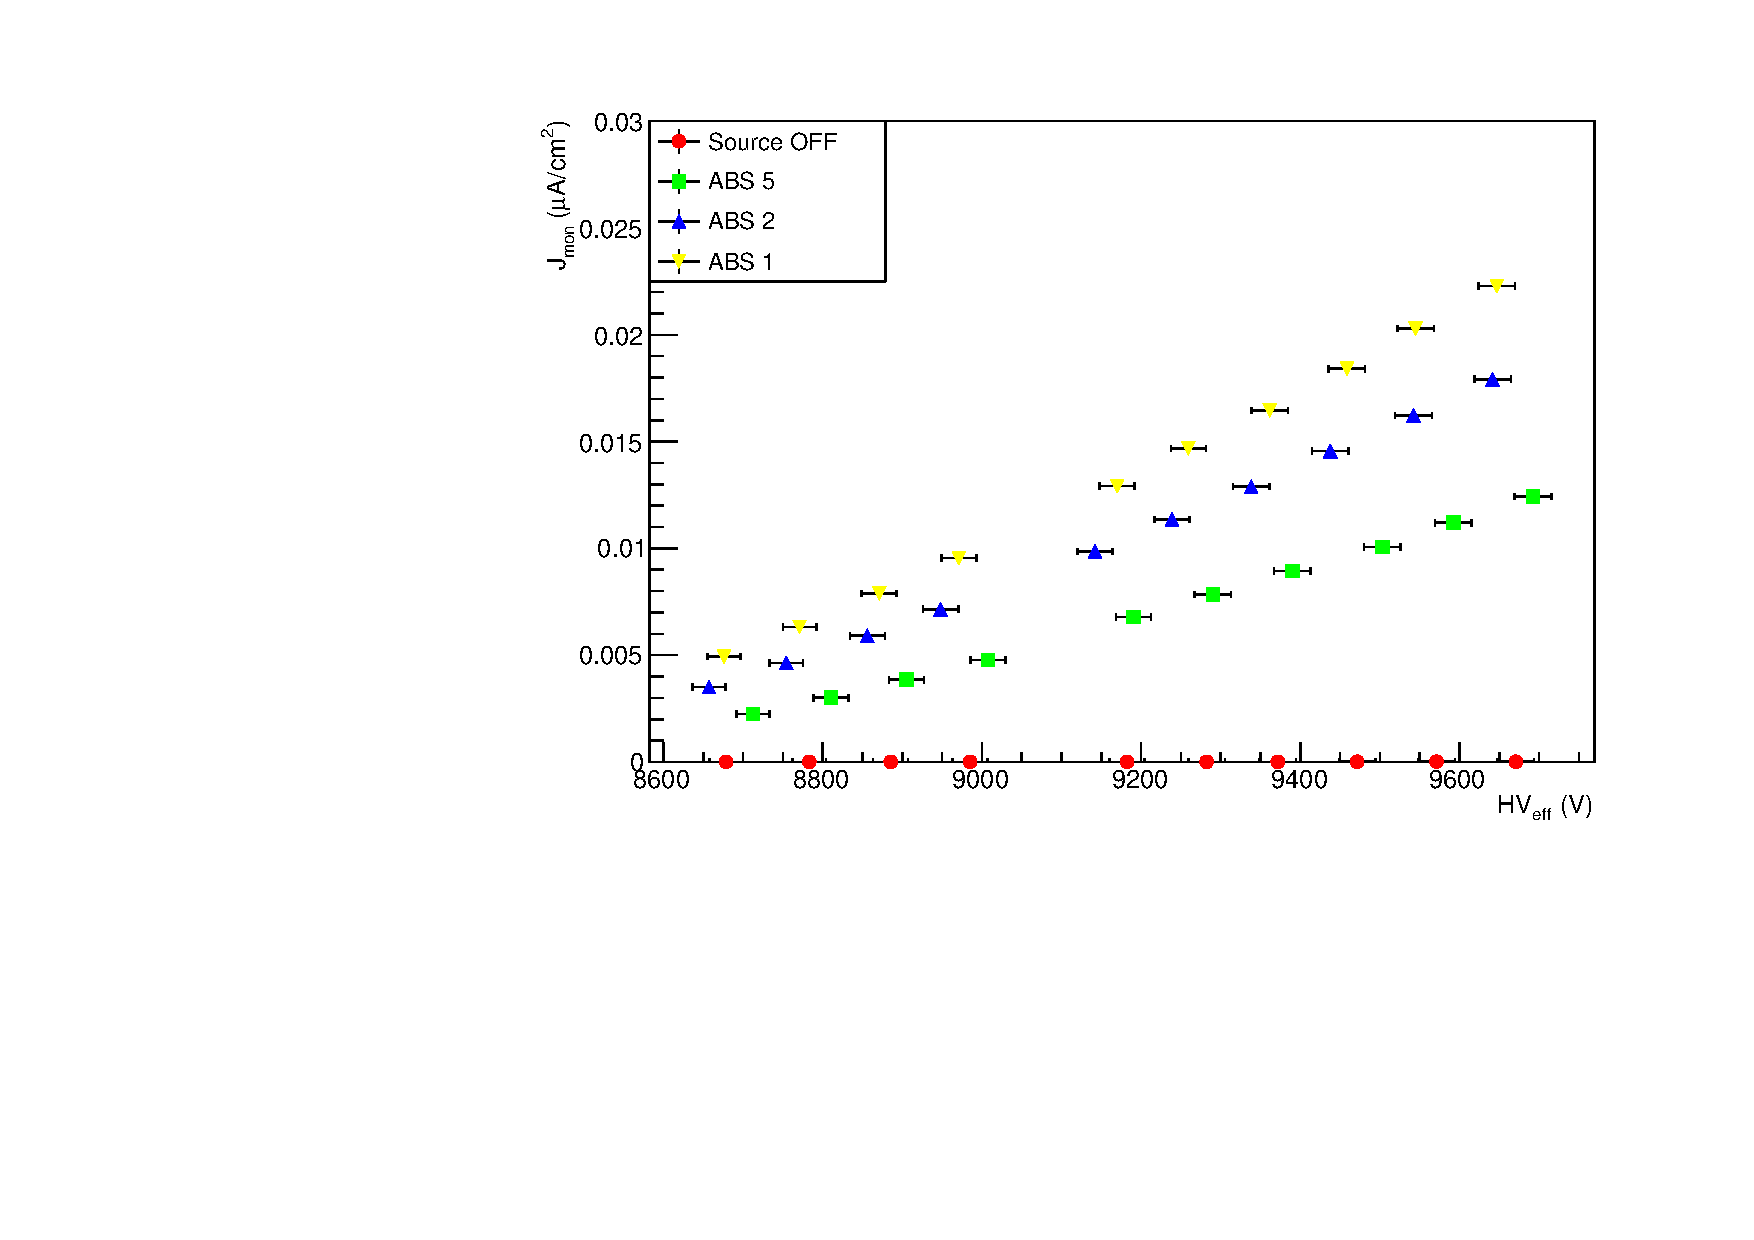
\includegraphics[width = 0.7\plotwidth]{fig/chapt5/Current-Density.pdf}
        	\caption{\label{fig:Charge:A}}
    	\end{subfigure}
    	\begin{subfigure}{0.5\linewidth}
			\centering
    		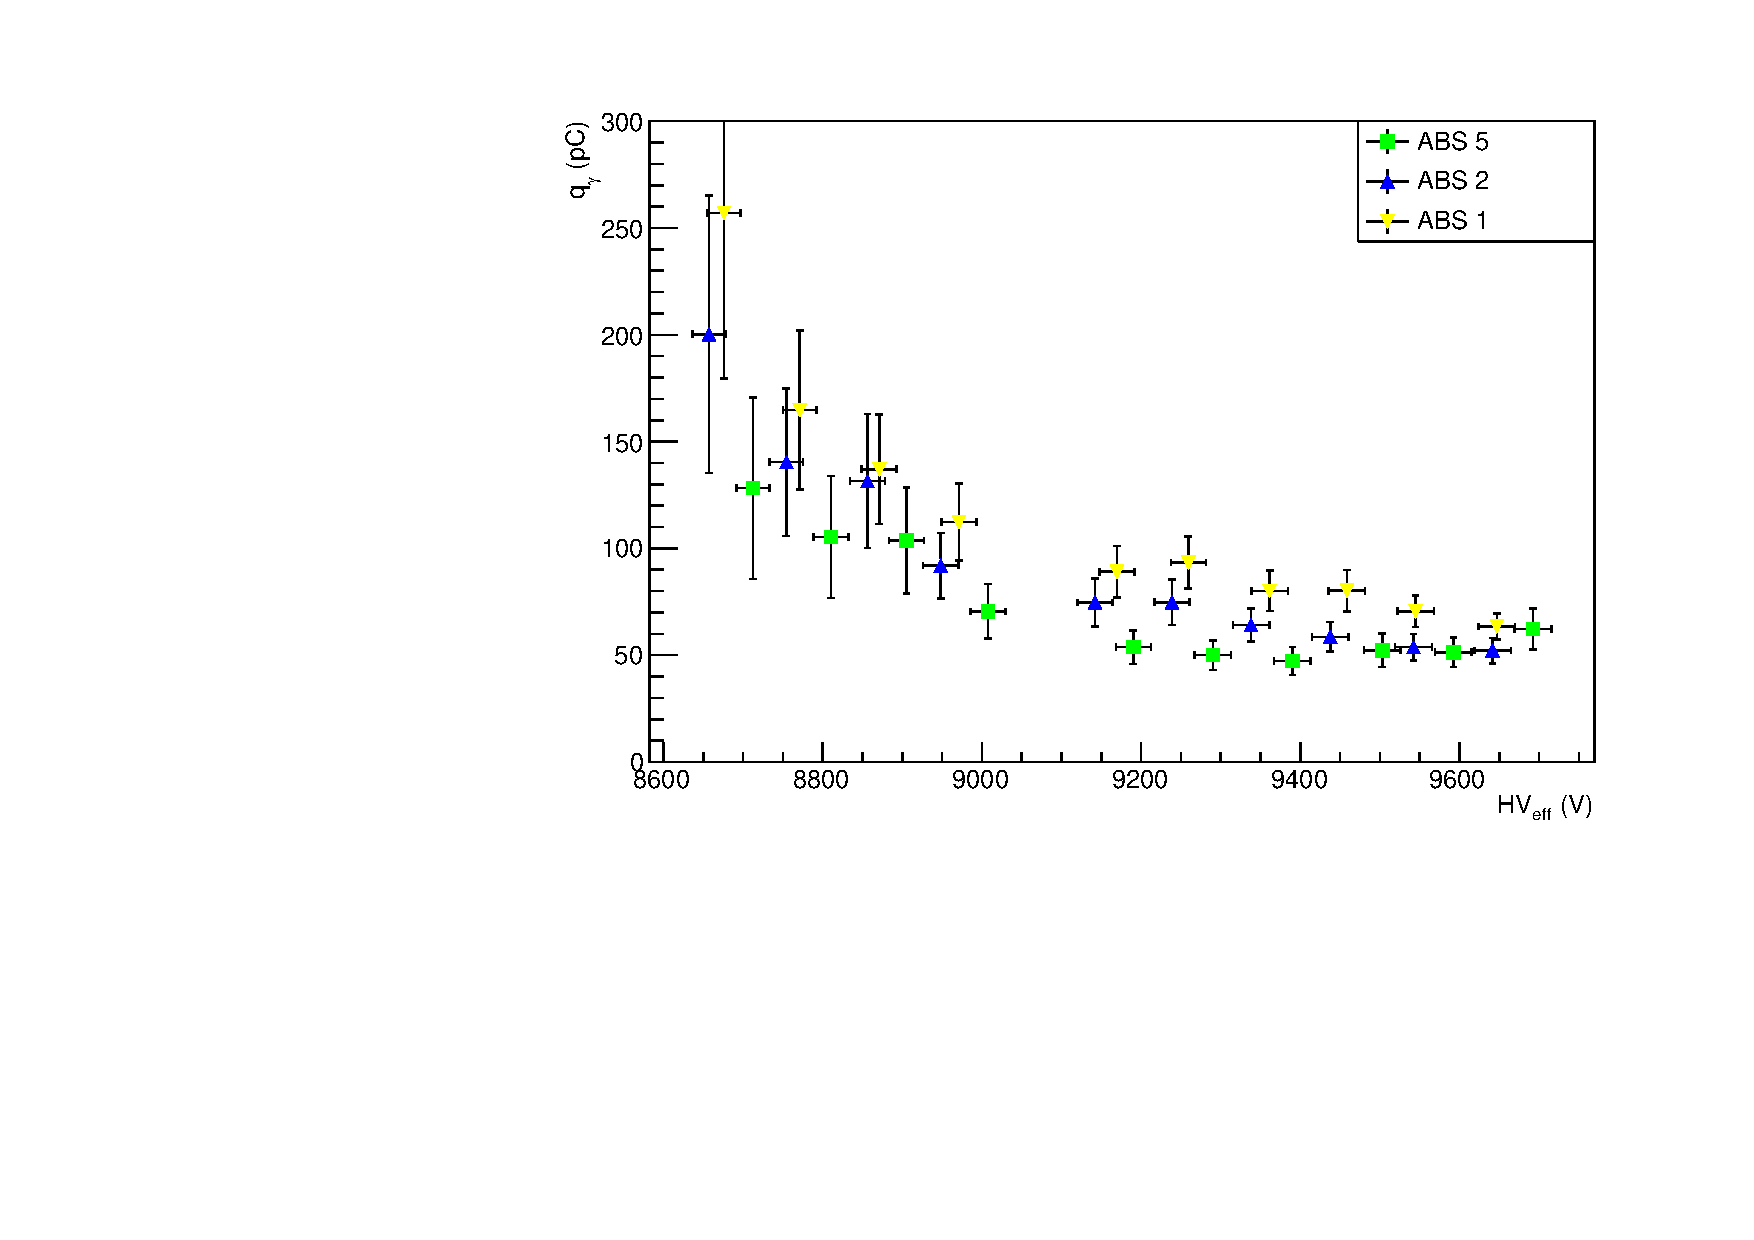
\includegraphics[width = 0.7\plotwidth]{fig/chapt5/Charge-per-gamma.pdf}
        	\caption{\label{fig:Charge:B}}
    	\end{subfigure}
		\caption{\label{fig:Charge} Current density~\subref{fig:Charge:A} and charge deposition per gamma avalanche~\subref{fig:Charge:A}, defined as the current density normalized to the measured rate taken from Figure~\ref{fig:GIFRate:A} as a function of the effective high voltage in chamber \texttt{RE-4-2-BARC-161} measured at GIF with Source ON using different absorber settings: ABS 5 (green), ABS 2 (blue) and ABS 1 (yellow).}
	\end{figure}
	
	Overall, working at GIF has been a rewarding experience as it offered CMS RPC R\&D team the possibility to start developing the necessary skills and tools that would become the core of GIF++ experiment. The quality of the results can be argued both due to the little robustness of the experimental setup and the lack of available statistics to draw conclusions from, bringing large errors on the final result. The confrontation of the data to known results pointed to a failure in correctly measuring the $\gamma$ rate at working voltage and, hence, to an overestimation of the charge per avalanche and of the drift of working voltage with increasing rate. Nevertheless, the prototypes of DAQ and offline analysis tools proved to be reliable.

\section{Longevity tests at \acs{GIF++}}
\label{chapt5:sec:GIFpptests}

	\subsection{Selection and characterization of CMS RPCs for longevity at GIF++}
	\label{chapt5:ssec:selection}

	In the perspective of future upgrades of LHC that would bring detectors to be operated in a high irradiation environment, the \acl{GIF++} of CERN was first proposed in 2009~\cite{GIF++2009}. The GIF++ would thus provide all LHC R\&D teams working on behalf of the different LHC experiment with a facility to perform longevity studies using a very intense Cesium gamma source.
	
	\begin{figure}[H]
    	\begin{subfigure}{0.5\linewidth}
			\centering
    		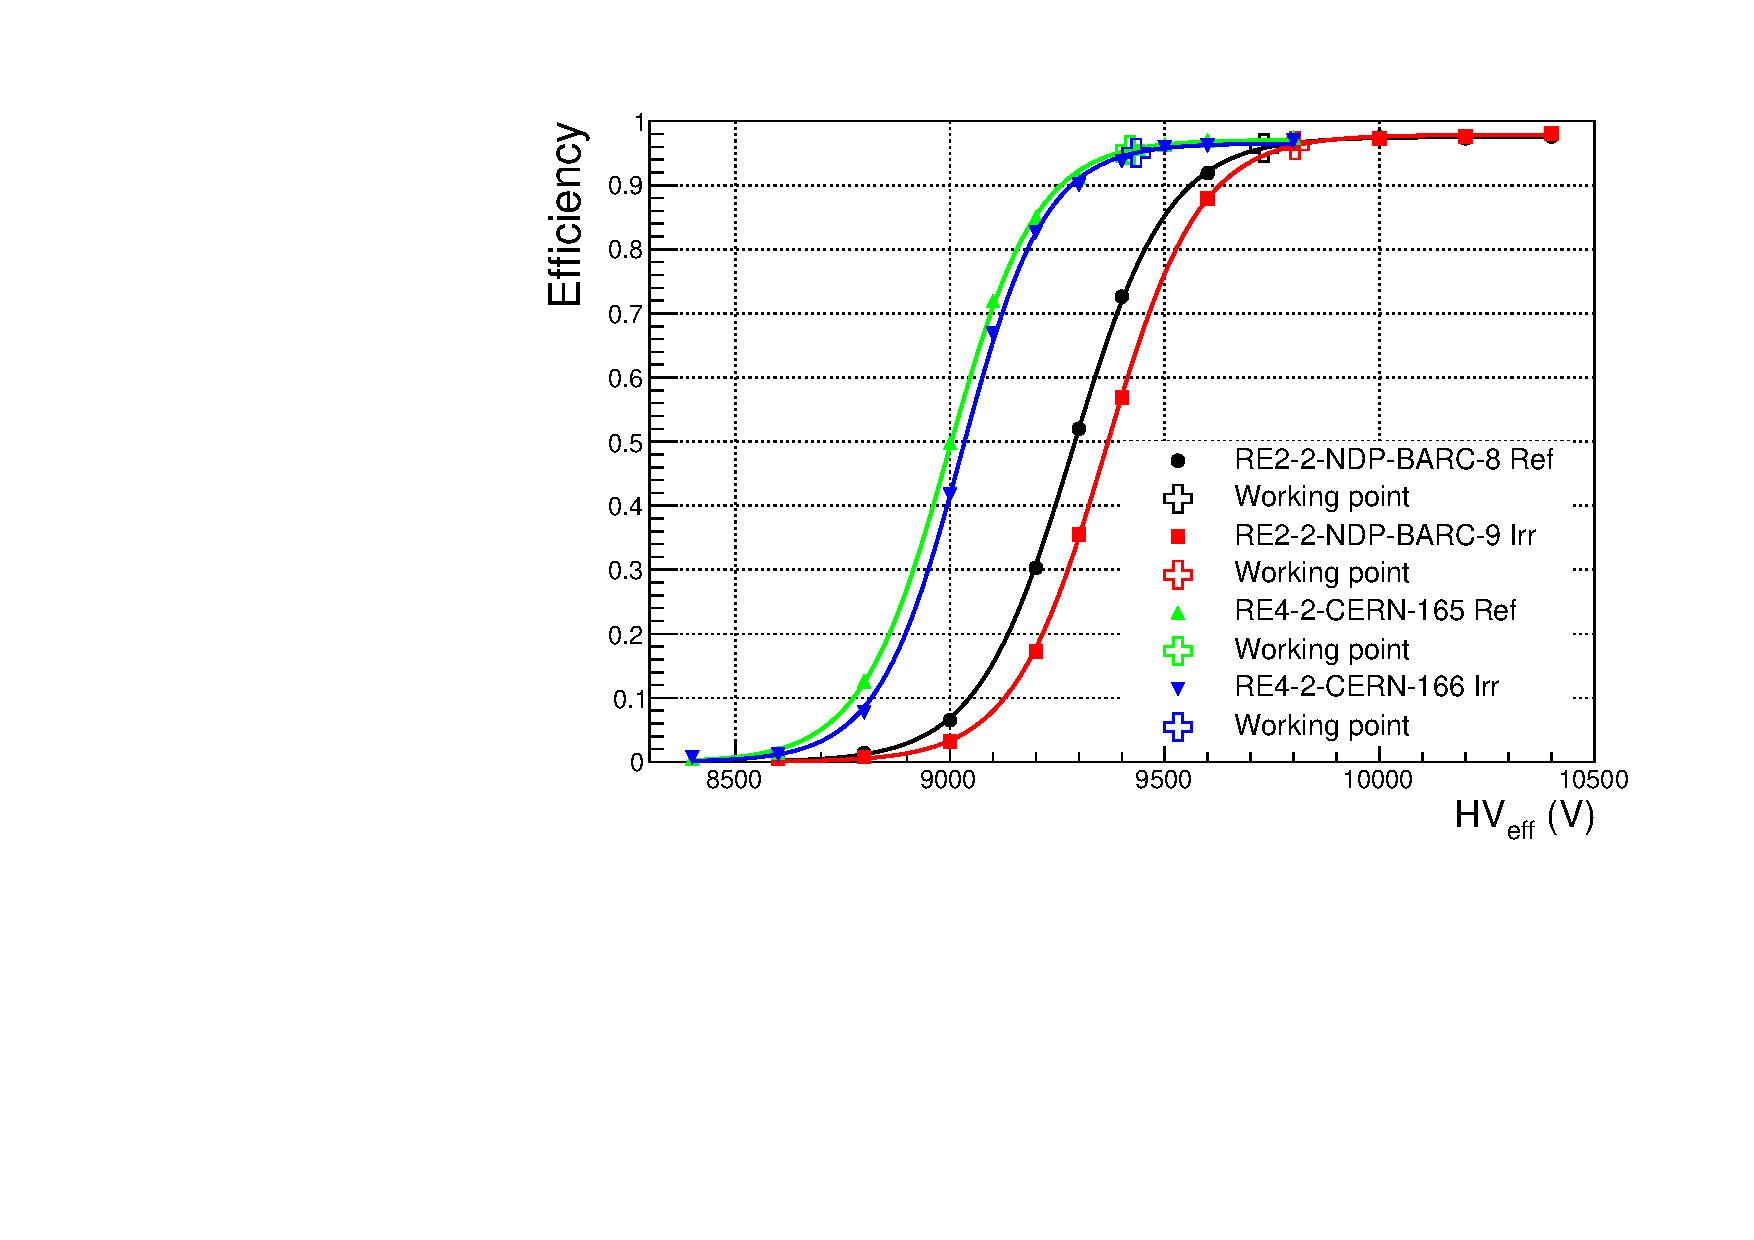
\includegraphics[width = \linewidth]{fig/chapt5/Consolidation-Efficiency.pdf}
        	\caption{\label{fig:consolidation:A}}
    	\end{subfigure}
    	\begin{subfigure}{0.5\linewidth}
			\centering
    		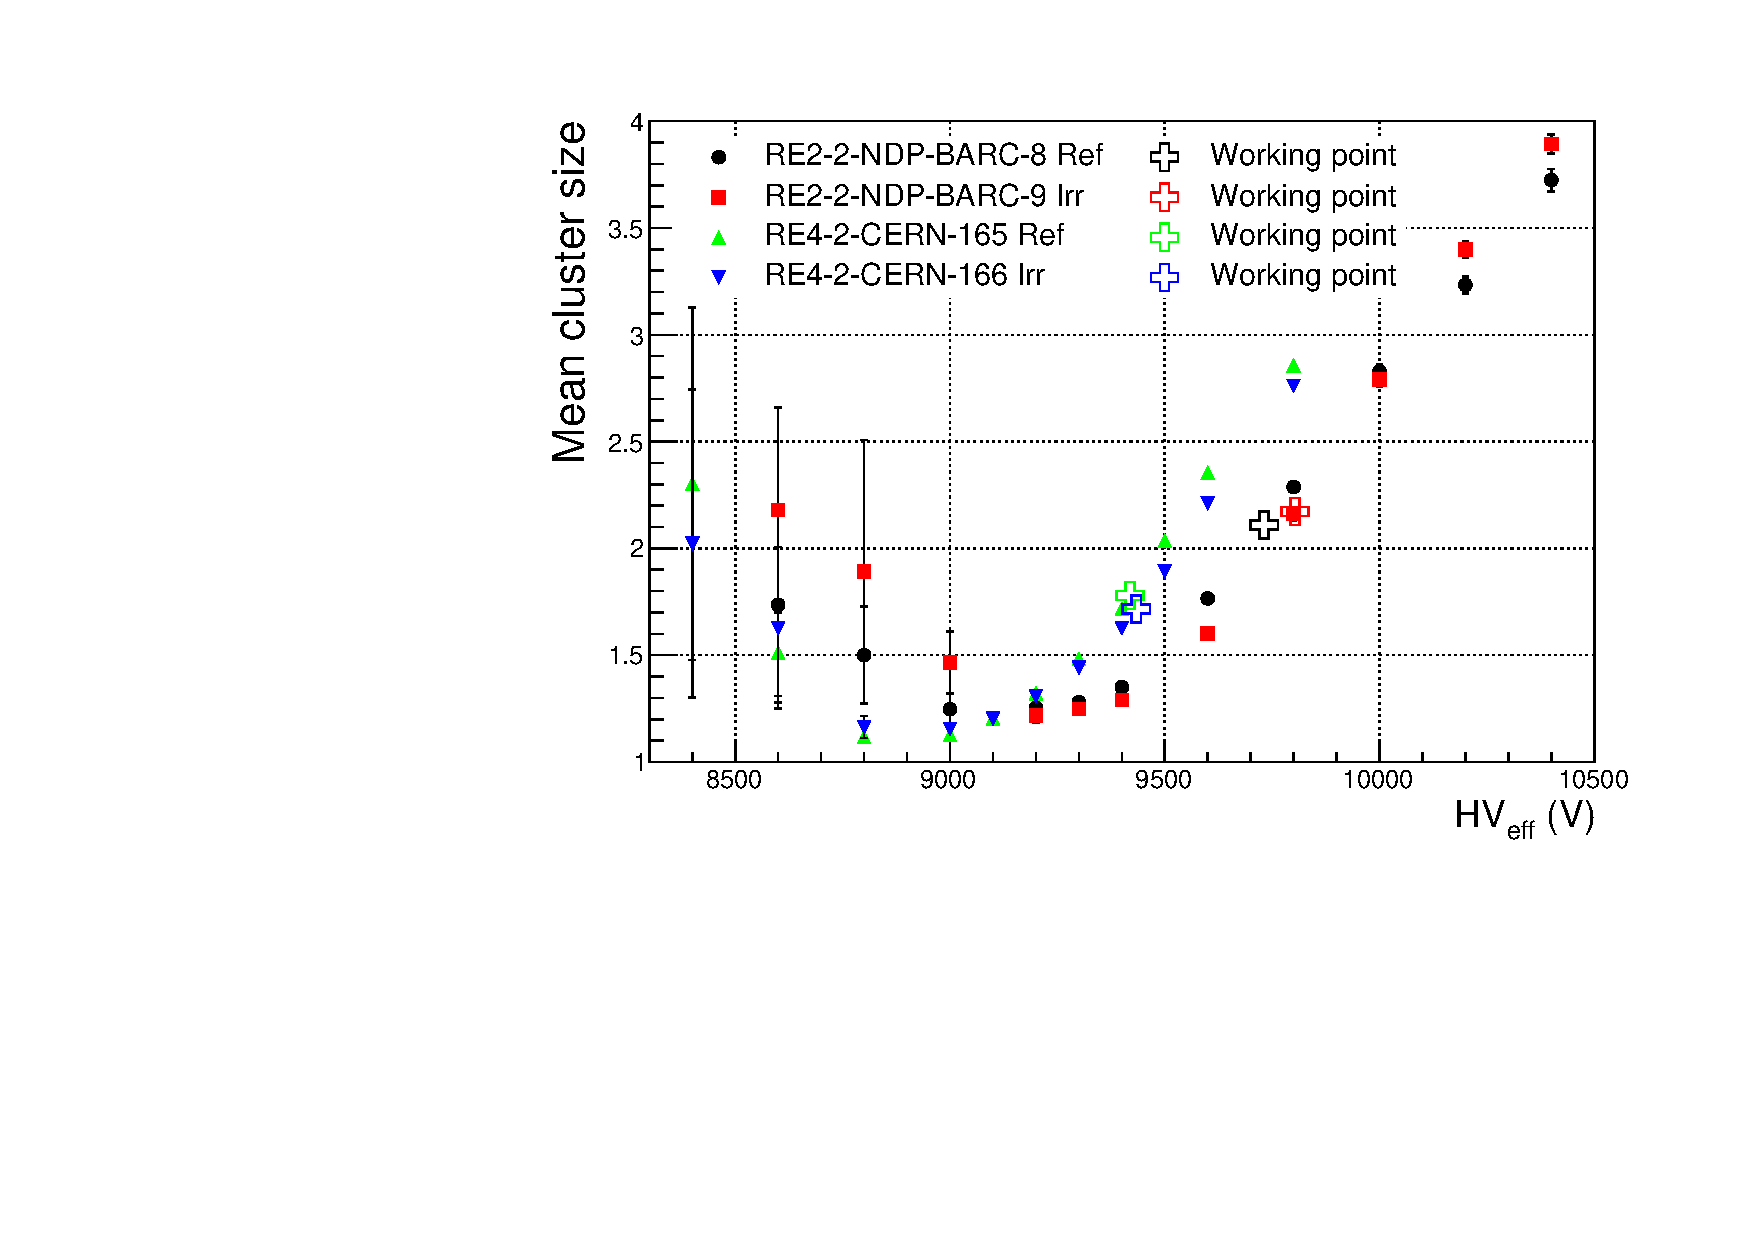
\includegraphics[width = \linewidth]{fig/chapt5/Consolidation-Cluster-Size.pdf}
        	\caption{\label{fig:consolidation:B}}
    	\end{subfigure}
    	\begin{subfigure}{0.5\linewidth}
			\centering
    		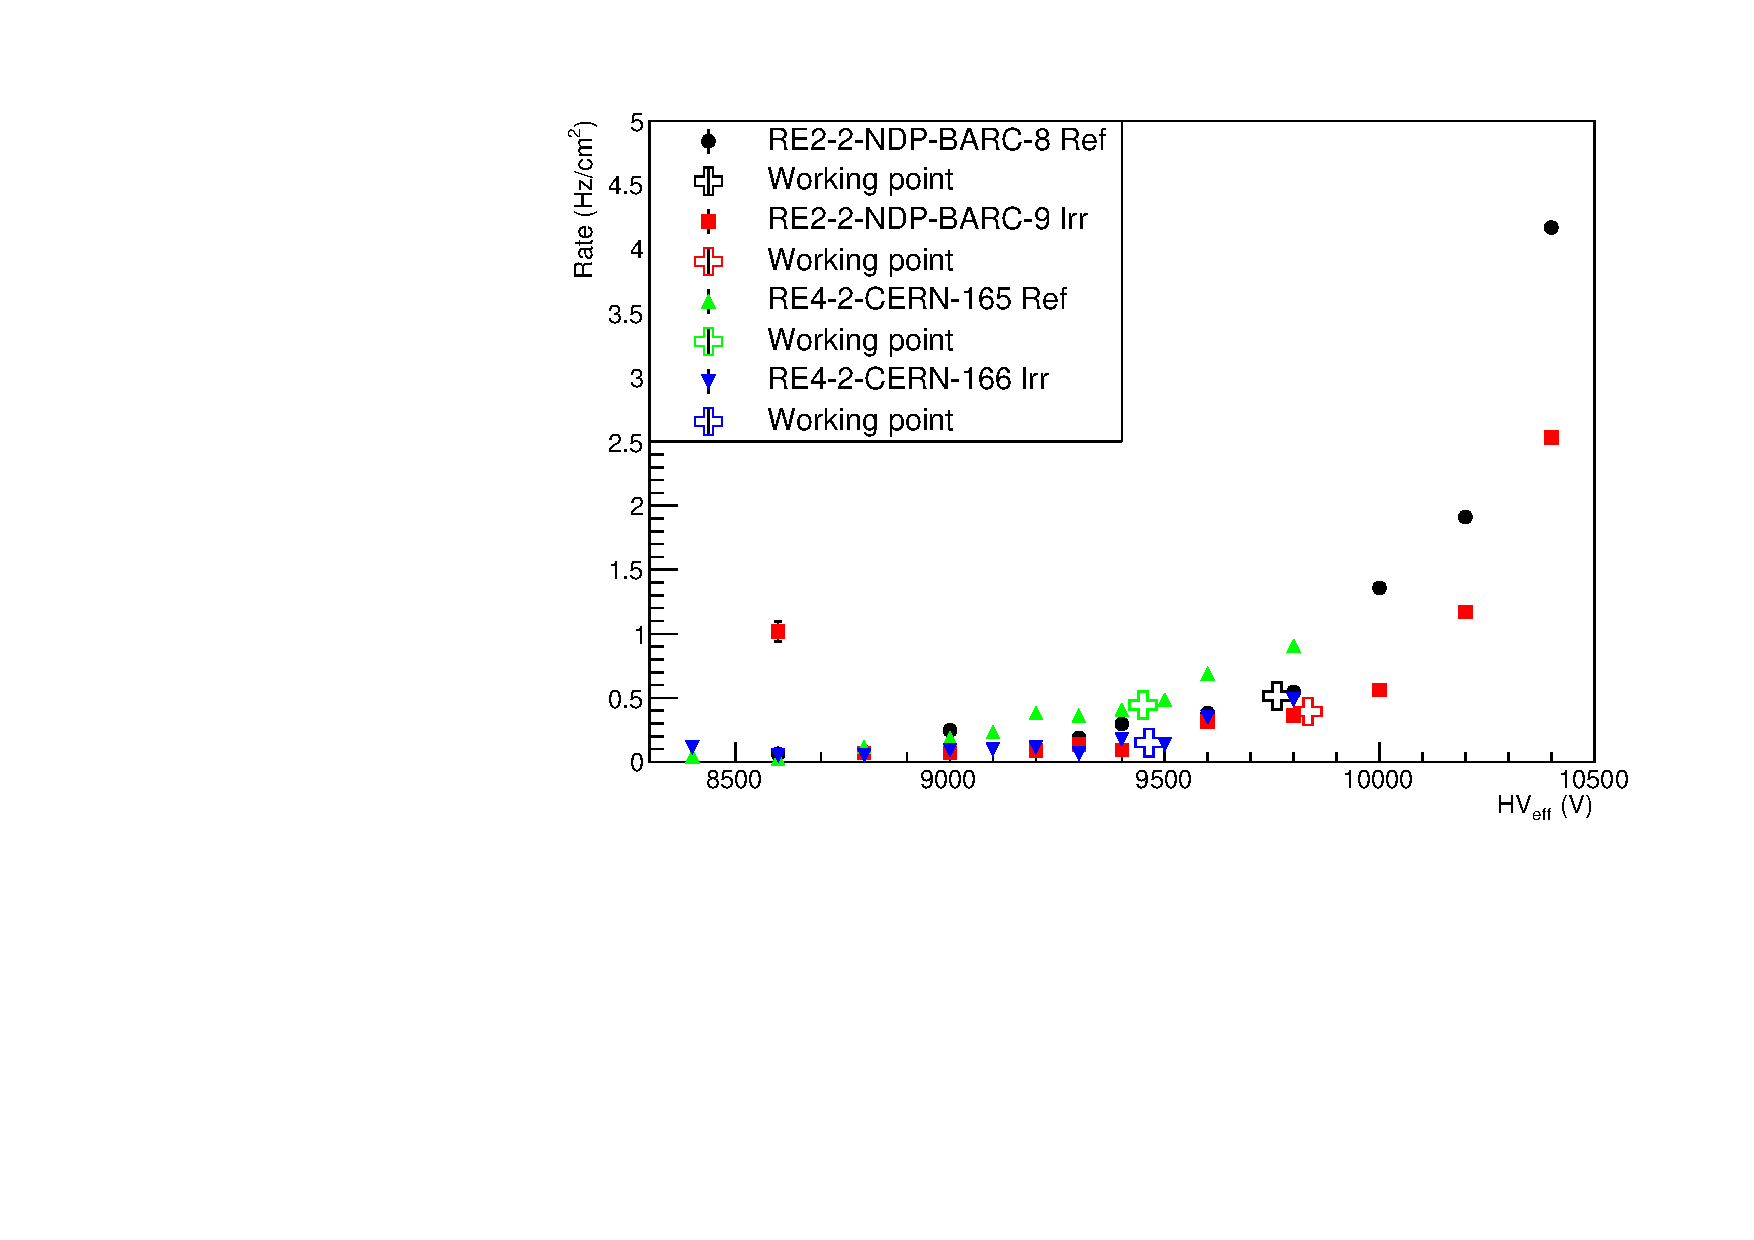
\includegraphics[width = \linewidth]{fig/chapt5/Consolidation-Noise-Rate.pdf}
        	\caption{\label{fig:consolidation:C}}
    	\end{subfigure}
    	\begin{subfigure}{0.5\linewidth}
			\centering
    		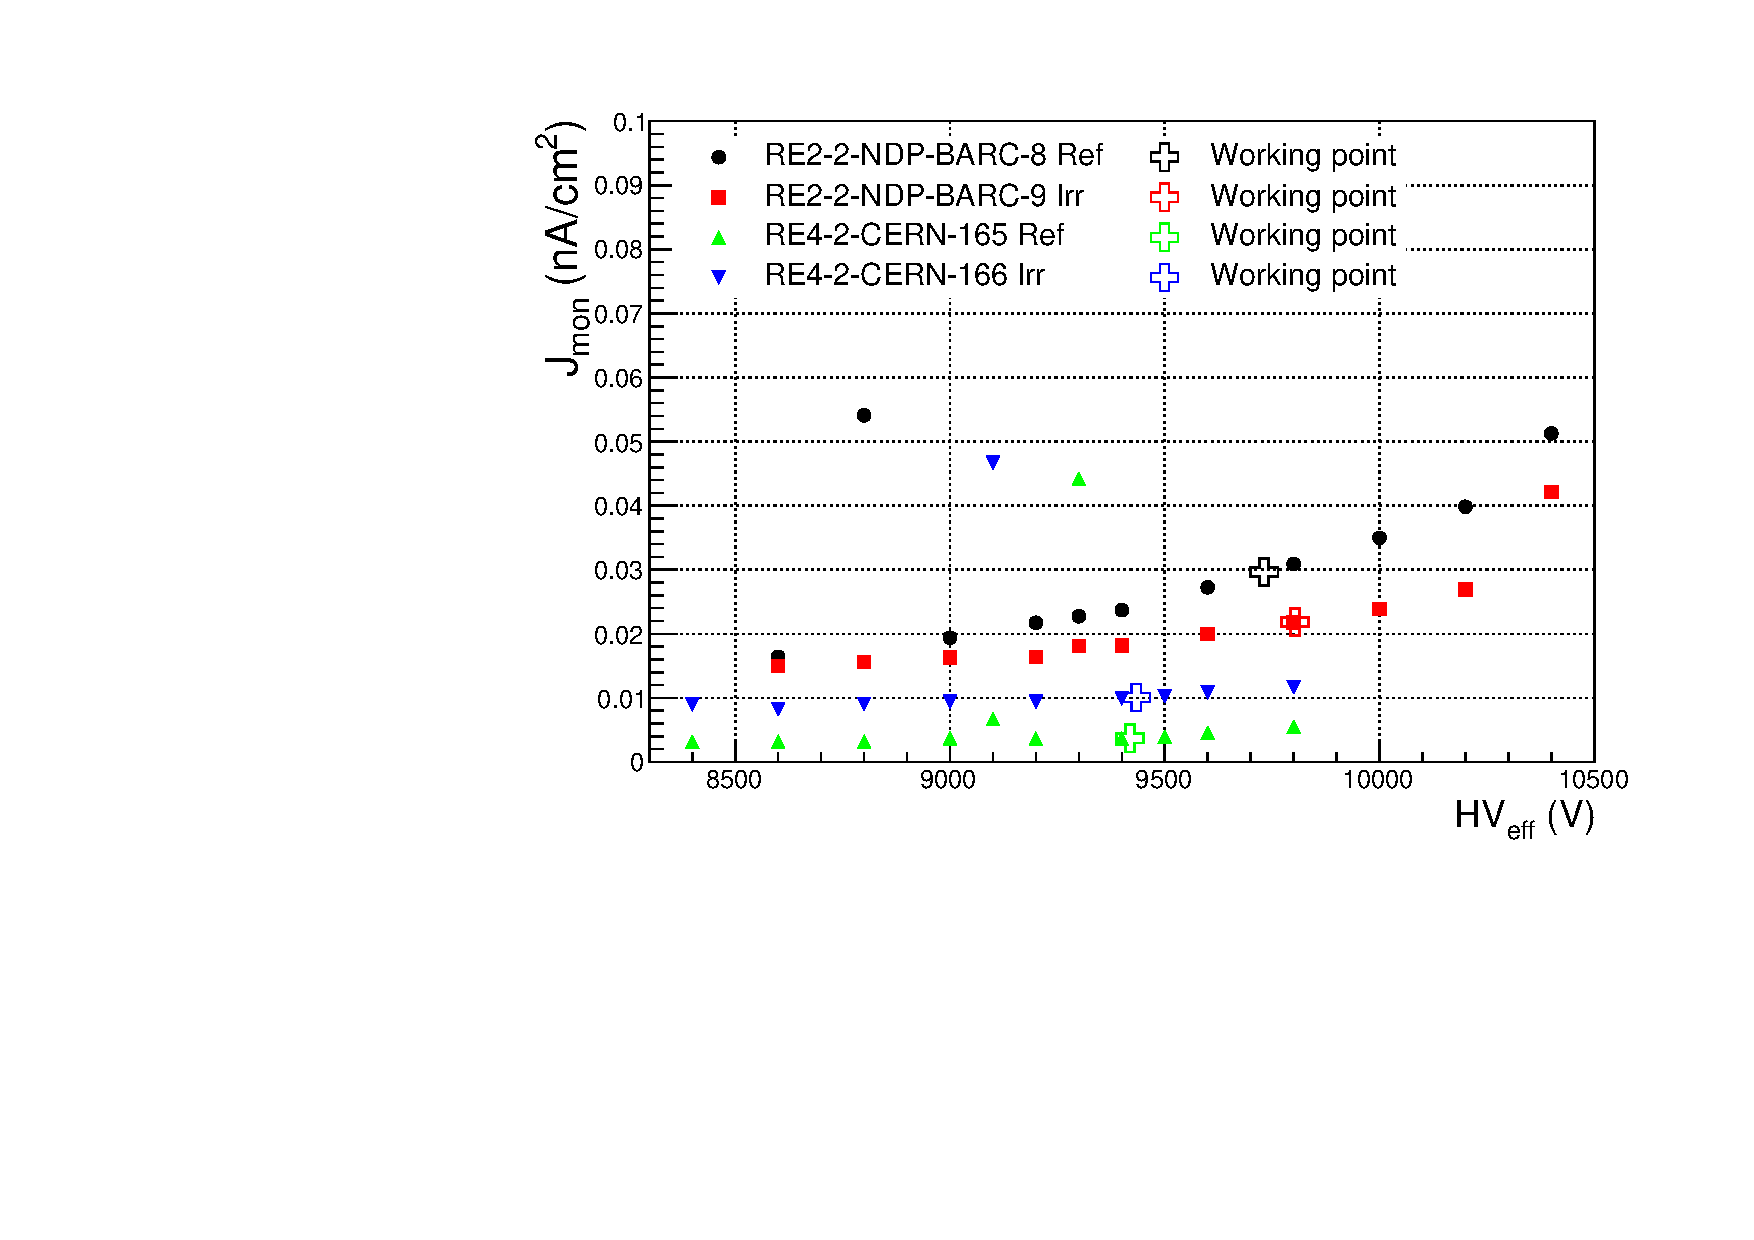
\includegraphics[width = \linewidth]{fig/chapt5/Consolidation-Current-Density.pdf}
        	\caption{\label{fig:consolidation:D}}
    	\end{subfigure}
		\caption{\label{fig:consolidation} Characterization of CMS RPC detectors foreseen to be used at GIF++ for longevity studies of the present system. Using cosmic muons, efficiency~\subref{fig:consolidation:A} and cluster size~\subref{fig:consolidation:B} were measured as well as noise rate~\subref{fig:consolidation:C} and current density~\subref{fig:consolidation:D}. For each detector, the working voltage, defined as in Formula~\ref{eq:KneeWP} after LS1, was extracted from sigmoid fits performed in Figure~\subref{fig:consolidation:A} and the values of efficiency, cluster size, noise rate and current density at this voltage are reported using open crosses.}
	\end{figure}
	
	In the specific case of CMS RPC, the longevity studies imply a constant irradiation of selected detectors in order to accumulate a charge equivalent to what is expected during HL-LHC, i.e. a charge of \SI{0.8}{C/cm^2} according to Figure~\ref{fig:RPC-HL-LHC} including a safety factor 3. Other detectors are left non-irradiated to be used as references. Throughout the irradiation campaign, the performance of the irradiated and reference detectors will be periodically probed using the high intensity H4 muon beam. Dedicated test beam periods will be used to measure the efficiency and gamma rate at the level of the detectors. Different source absorber settings will test the rate capability of CMS RPCs, that needs to be certified above \SIrate{600}. Using a muon beam will also help identifying signs of ageing in the case the performance of the irradiated detectors diverges from those of the reference detectors with increasing accumulated charge. Other than the performance of the detectors, signs of ageing could come from increasing dark current that would be related to local ageing of the electrodes triggered by the increased hydrofluoric acid ($HF$) production in an irradiated environment. $HF$ is produced by the decomposition of $C_2H_2F_4$ molecules during the charge multiplication process and leads to increased dark current and noise in Bakelite RPCs treated with linseed oil. This effect is strongly reinforced by the presence of UV photons~\cite{GUIDA2008,BELLINI2008}. A close monitoring of the current driven by the detectors will then be necessary as well as dedicated periodical electrode resistivity measurements and chromatography analyses on the gas exhaust.
	
    As the maximum background in CMS is found in the endcap disks, the choice was made to focus the GIF++ longevity studies on endcap chambers. Most of the RPC system was installed in 2007. Nevertheless, the large chambers in the fourth endcap (RE4/2 and RE4/3) have been installed during LS1 in 2014. The HPL of these two different productions possibly having slightly different properties, four spare chambers of the present system were selected. From the original CMS RPC system, two RE2/2 spares were selected along two RE4/2 spares from the newest detectors. Having two chambers of each type allowed to always keep one of them non-irradiated as reference. Due to the limited gas flow in GIF++, the RE4 chamber remained non-irradiated until end of November 2016 when the longevity studies could finally be started on those chambers.
    
    The performance of the chambers prior to the start of the longevity campaign was characterized in Ghent before their transportation to CERN for installation in the GIF++. The results of the characterization are showed in Figure~\ref{fig:consolidation} and summarized in Table~\ref{tab:consolidation}. A clear difference in performance for both types of chambers is observed as the working voltages of the newest chambers, of type RE4, are 300 to \SI{400}{V} lower to the older chambers indicating that the gap thickness of RE4 detectors could be thinner. This conclusion could as well be supported by the lower cluster size at working voltages that are also smaller in RE4 chambers. Even though the measured currents are low, RE4 detectors draw less current without irradiation than RE2 detectors pointing to a difference in electrode resistivity that were produced at different moments. Efficiency and noise rate levels are of the same order of magnitude for both type of RPCs.
	
	\begin{table}[H]
		\hspace*{-1cm}
		\begin{tabular}{|*{5}{c|}}
			\hline
			RPC & \footnotesize{\texttt{RE2-2-NPD-BARC-08}} & \footnotesize{\texttt{RE2-2-NPD-BARC-09}} & \footnotesize{\texttt{RE4-2-CERN-165}} & \footnotesize{\texttt{RE4-2-CERN-166}} \\
			\hline
			Used as & Reference & Irradiation & Reference & Irradiation \\
			\hline
			$HV_{WP}$ (\si{V}) & \numerror{9732}{6} & \numerror{9803}{6} & \numerror{9419}{5} & \numerror{9434}{5} \\
			\hline
			Efficiency at WP & \numerror{96.2}{0.3} & \numerror{96.6}{0.3} & \numerror{95.9}{0.3} & \numerror{95.5}{0.3} \\
			\hline
			Cluster size at WP & \numerror{2.19}{0.04} & \numerror{2.27}{0.05} & \numerror{1.88}{0.04} & \numerror{1.80}{0.04} \\
			\hline
			Noise at WP (\sirate) & \numerror{0.51}{0.01} & \numerror{0.39}{0.01} & \numerror{0.44}{0.00} & \numerror{0.15}{0.01} \\
			\hline
			$J^{WP}$ (\si{pA/cm^2}) & \numerror{30.1}{0.1} & \numerror{22.2}{0.1} & \numerror{3.8}{0.0} & \numerror{10.2}{0.0} \\
			\hline
		\end{tabular}
		\caption{\label{tab:consolidation} Summary of the characterization measurement performed in Ghent on CMS RPC detectors foreseen to be used at GIF++ for longevity studies of the present system. For each detector, the working voltage, defined as in Formula~\ref{eq:KneeWP}, was extracted from sigmoid fits performed in Figure~\ref{fig:consolidation:A}. The values of efficiency, cluster size, noise rate and current density at this voltage are reported.}
	\end{table}

	\subsection{RPC test setup}
	\label{chapt5:ssec:GIFppSetup}
	
	For an easy manipulation of the detectors, a trolley with a structure containing slots in which the RPCs can be slid vertically was used and is referred to as \texttt{T1}. When in position, each chamber is in a plane perpendicular to the beam line and the source flux as can be seen through Figure~\ref{fig:GIFppSetup}, and receives a uniform irradiation. Moreover the trolley allows for easy movement of the system. Indeed, the position of the trolley varies according to the specific measurements that are being done.
	
	\begin{figure}[H]
    	\begin{subfigure}{0.5\linewidth}
			\centering
    		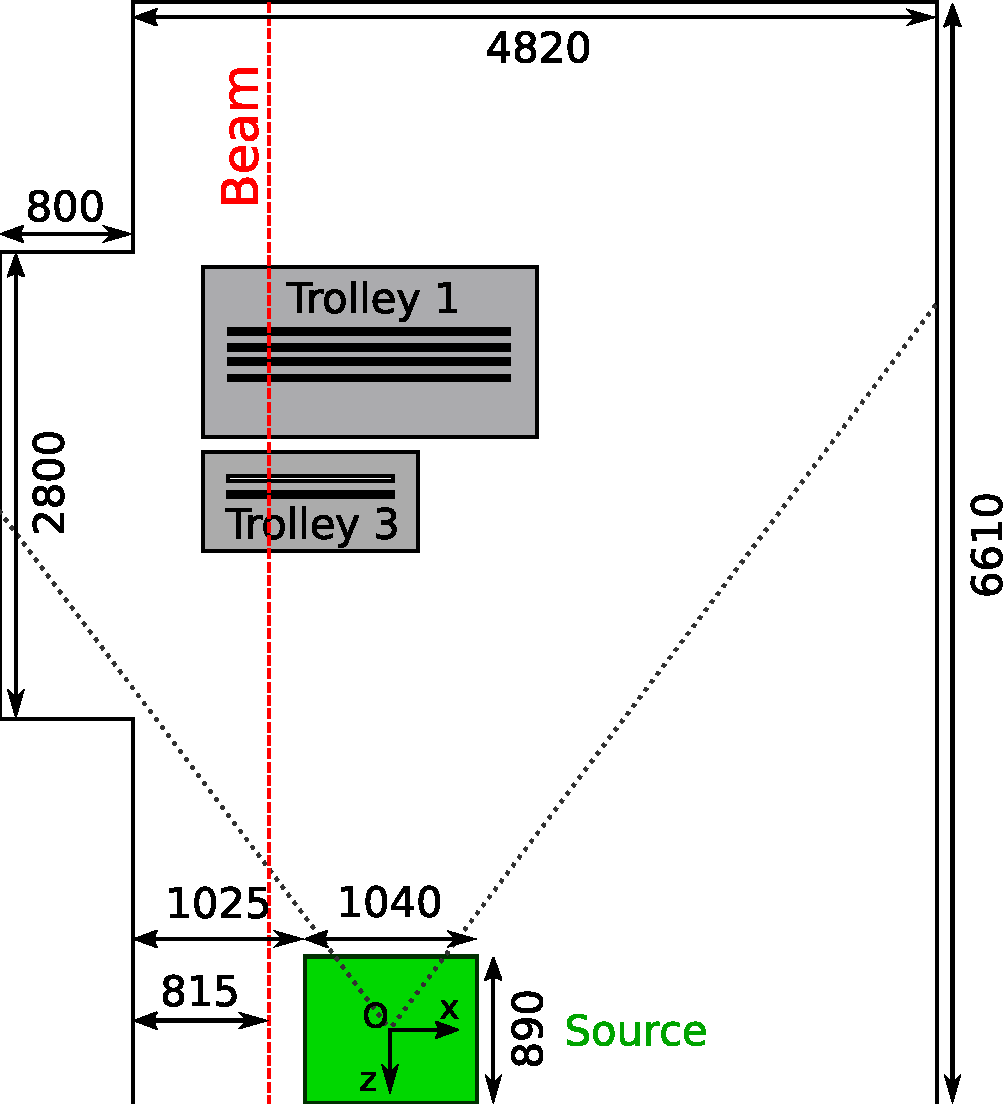
\includegraphics[height = 65mm]{fig/chapt5/GIFpp-Setup-A.pdf}
        	\caption{\label{fig:GIFppSetup:A} Test beam position}
    	\end{subfigure}
    	\begin{subfigure}{0.5\linewidth}
			\centering
    		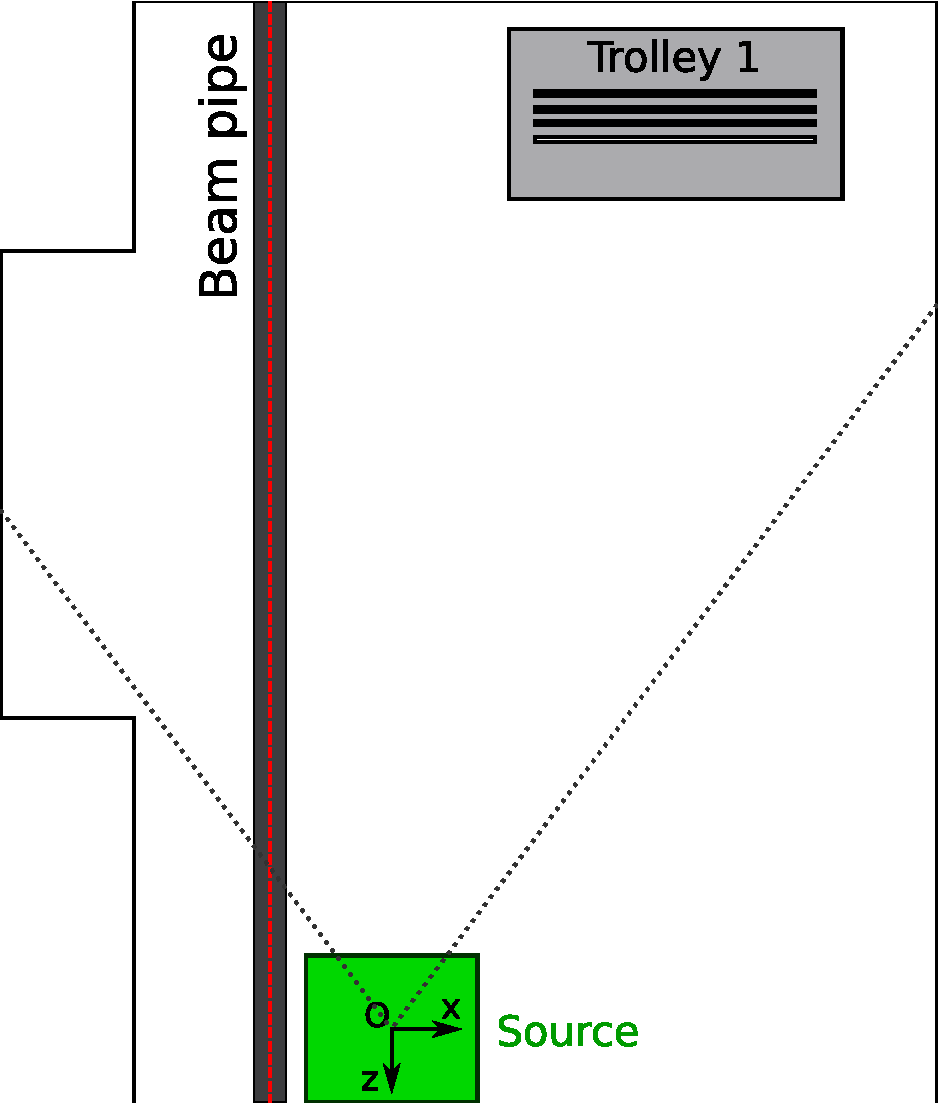
\includegraphics[height = 65mm]{fig/chapt5/GIFpp-Setup-B.pdf}
        	\caption{\label{fig:GIFppSetup:B} Ageing position}
    	\end{subfigure}
    	\begin{subfigure}{\linewidth}
    		\vspace*{5mm}
			\centering
    		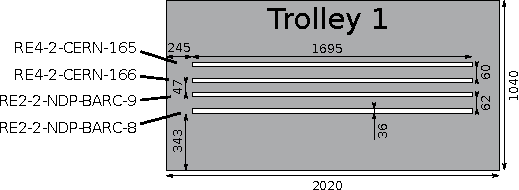
\includegraphics[width = 0.8\plotwidth]{fig/chapt5/GIFpp-T1.pdf}
        	\caption{\label{fig:GIFppSetup:C}}
    	\end{subfigure}
		\caption{\label{fig:GIFppSetup} CMS RPC setup inside the GIF++ bunker during test beam~\subref{fig:GIFppSetup:A} and ageing periods~\subref{fig:GIFppSetup:B}. The space in between the RPCs and the source is usually used by other detectors while the space in between \texttt{T1} and the upstream wall is not filled. Due to the presence of the beam pipe, the trolley is moved away from the beam line during irradiation periods and placed further away from the source for less intense irradiation. The position of the trolley can vary due to the use of the space by other setups and is then not exact. Nonetheless, the position of the chambers in the trolley is fixed and given in Figure~\subref{fig:GIFppSetup:C}.}
	\end{figure}
	
	During the dedicated test beam periods, the GIF++ experiments are in control of the muon beam. The trolley is placed in the upstream region of the bunker, in the beam line at a distance of generally \SI{3.4}{m} from the source, as described through Figure~\ref{fig:GIFppSetup:A}. At this distance, the simulated gamma current is the order of \Sci{5}{6} \siflux. The CMS RPC detectors are the furthest away from the source as other detectors need to be certified at higher background rates. Depending on the needs of the other experiments at the GIF++, the trolley position of the trolley can be pushed as far as \SI{4.1}{m} from the source. An additional trolley, referred to as \texttt{T3}, contains iRPCs and is placed between the source and the \texttt{T1} trolley. Indeed, iRPCs need to be certified at higher rates and thus need to be placed closer to the source to receive a stronger irradiation using the same absorber settings. The space on \texttt{T1} being limited, the tracking RPCs used for extra offline information during the analysis are placed on the same trolley as the iRPCs. they are kept at full efficiency at all time to reconstruct muon tracks and to correlate them with hits recorded in \texttt{T1} chambers. The beam trigger system is composed of three scintillators. Two are placed outside on each side of the bunker and of the third scintillator is placed in the beam line in between \texttt{T1} and the wall.
	
	Most of the year, outside of these test beam periods, \texttt{T1} is placed in the so called \textit{ageing position} corresponding to the furthest position at approximately \SI{4.7}{m} from the source outside of the beam line before August 2019. At such a distance, the simulated gamma current is the order of \Sci{3}{6} \siflux. Following the extension of the upstream area in August 2019, the trolley was pushed approximately \SI{1}{m} away at a distance of \SI{5.7}{m} to the source, corresponding to a simulated gamma current of the order of \Sci{2}{6} \siflux. During periods where GIF++ doesn't have the control of the beam, the beam line needs to stay clear so that a beam tube can be installed through the bunker, as can be seen in Figure~\ref{fig:GIFppSetup:B}. The reason for placing the chambers as far as possible from the source comes from the too high irradiation delivered by the source during the irradiation periods where all the other groups having placed detectors in the bunker require as much charge integration as possible. Hence, the source is operated without any absorbers. On the contrary, during the test beam periods, all the groups working in GIF++ are interested in operating the source using various absorber settings to study the performance of their detectors under different irradiation conditions. \texttt{T1} RPCs are kept at a stanby voltage of \SI{6500}{V} when the other groups need to work with ABS 1 due to the proximity of the trolley to the source compared to ageing periods.
	
	From the bunker area, long cables and pipes running through the wooden floor connect the detectors to the service area, visible in Figure~\ref{fig:GIFpp-Layout}. The service area hosts all the high and low voltage power supplies, the TDCs and computers used for data acquisition and preliminary offline analysis. The gas system required for the gaseous detectors installed in GIF++ can also be found in the service area~\cite{WEBDCS}.\\
	The detectors read-out is, as in the case of GIF, connected to \texttt{V1190A} VME TDCs communicating with the DAQ computer via a \texttt{V1718} VME bridge manufactured by \texttt{CAEN}. At the end of each data tacking, the preliminary analysis is run to fill the \acl{DCS} webpage, referred to as WebDCS, with \acf{DQM} histograms. The WebDCS is a custom made DCS application for the specific case of GIF++ RPCs. It provides online information about the environmental parameters in the bunker as well as the the state of each detector. A constant monitoring of all the environmental parameters, in different points of the bunker area, gas parameters, to control its composition, temperature and pressure, and of the voltages and currents delivered by the power supplies is performed and displayed on the homepage of the WebDCS interface. Moreover, it contains the database with all the RPC data in the form of \texttt{ROOT} files and of summary hisrograms. Hence, it is a useful tool for the shifters on duty in the control room located farther in the building, away from the beam lines.

	\subsection{GIF++ data flow}
	\label{chapt5:ssec:dataflow}
	
	At GIF++, the CMS RPC R\&D setup collects different types of data from the detector monitoring parameters, such as voltage and currents, the gas, source, and environmental parameters, and, of course, the TDC data related to the actual muon and gamma measurements. These different data sources correspond to three different data flows as presented in Figure~\ref{fig:dataflow}.
	
	The \textit{\acf{DIP} flow}, DIP being a communication system allowing for exchange of real-time information between systems~\cite{DIP}, concerns all the data coming from the gas composition, temperature and humidity, the environmental temperature and pressure, the source settings and the radiation monitoring sensors. At the experimental area, all data of interest for all of the users of the facility (source settings, radiation monitoring, gas composition at the exit of the gas mixer and general environmental information) are measured, distributed and also stored in the data of the experimental hall where is located the GIF++. Access to the database is done through DIP communication. The measurement of more specific data such as gas flow, temperature and humidity at the level of the detectors (upstream and downstream of the detectors) as well as environmental parameters has to be arranged by the users themselves. For this reason, several pressure, temperature and humidity sensors were installed on the gas distribution system of the RPC trolleys. The corresponding data flow, although not related to DIP itself, is saved together with the DIP data into the local CMS RPC database and displayed on the front page of the WebDCS. In the case any of the measured values go out of their optimal range, the WebDCS will produce corresponding alerts. The data are particularly important to perform the PT correction described in Section~\ref{chapt3:sec:PTcorrection} of Chapter~\ref{chapt3} and to stabilize the effective voltage of the detectors. Monitoring history plots are made using \texttt{JavaScript} are also displayed for easy access to past information, as shown in Figure~\ref{fig:DIP-monitoring}.

	\begin{figure}[H]
        \centering
		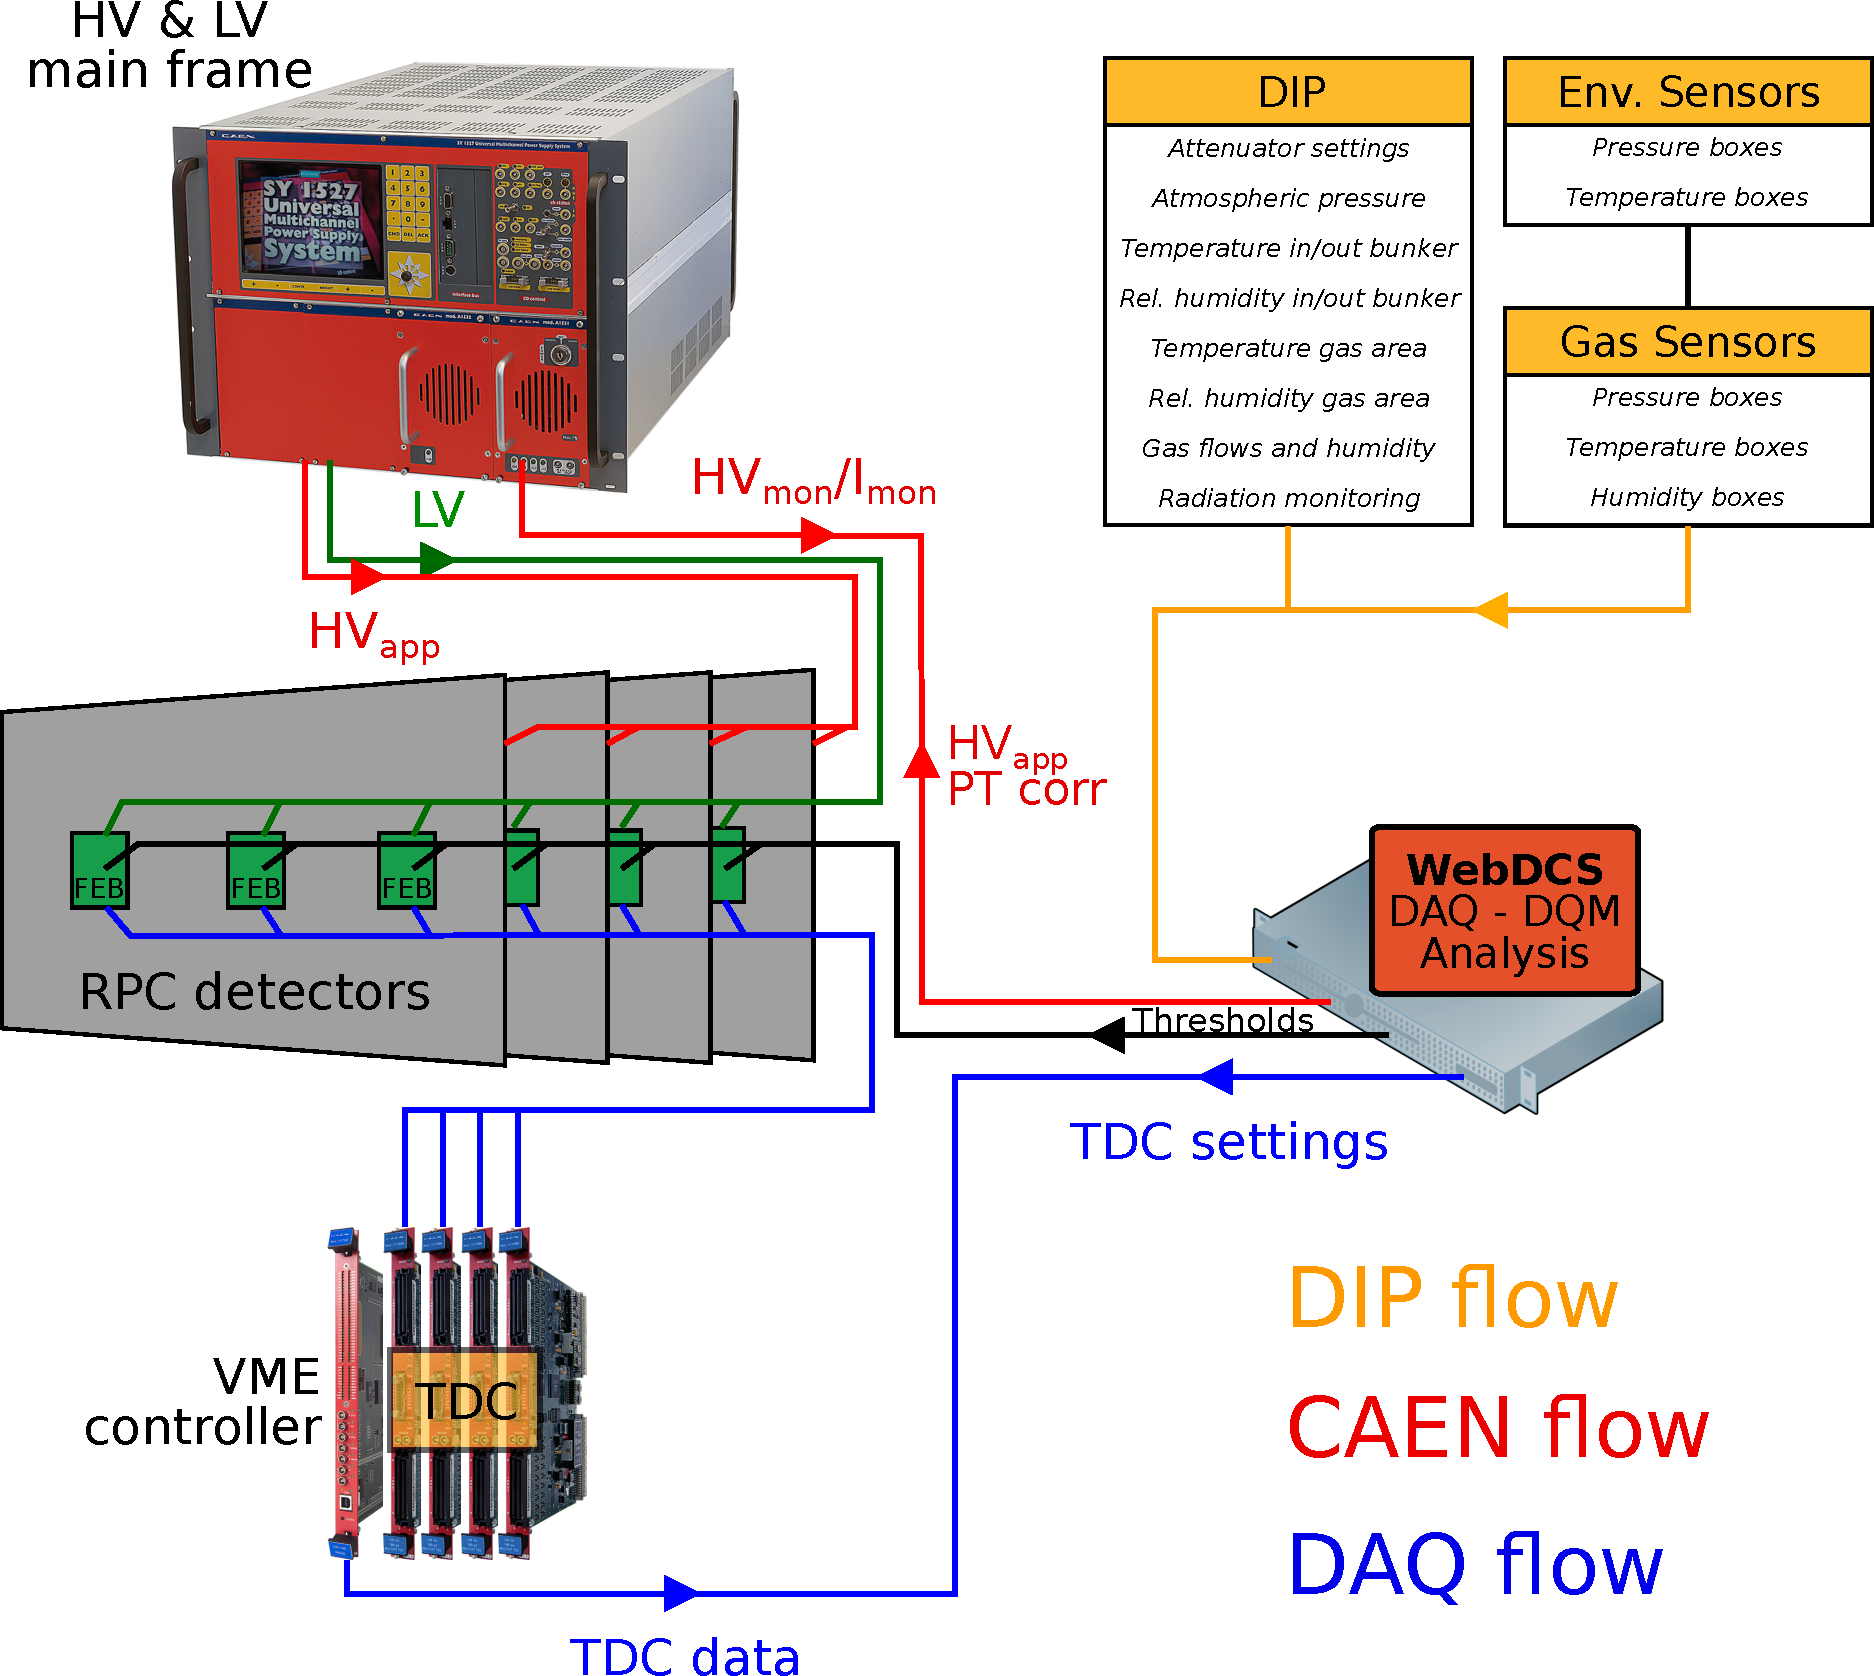
\includegraphics[width = 0.9\linewidth]{fig/chapt5/GIFpp-setup.pdf}
		\caption{\label{fig:dataflow} Visualisation of the main data flows in the CMS RPC setup at the GIF++. The yellow flow lines correspond to the DIP flow used for source, environmental and gas information. The red flow lines are for the CAEN flow through which the WebDCS communicates the voltages to be applied on the detectors using pressure and temperature information and retrieves the monitored voltages and currents. Finally, the blue flow lines correspond to the DAQ flow through which the RPC data is collected from the TDCs by the computer.}
	\end{figure}
	
	The data flow related to the monitoring of the detector high voltages and currents, referred to as \textit{CAEN flow} as a reference to the manufacturer of power supplies, is handled through direct communication between the DAQ computer and the power supply main frames. Finally, the DAQ flow concerns all data acquired through the use of the TDCs, i.e. all the muon or gamma event data recorded by the detectors under test at GIF++. It was already discussed that when a trigger signal is sent to a TDC module, the TDC saves all of the data located in a certain time window set around the time stamp of the signal. The trigger signal in the case of GIF++ can be a coincidence of the trigger scintillators or a signal from a pulse genrator. The DAQ computer extracts from the TDC buffers the list of fired channels and of associated time stamps for each trigger signal. The data is then used to reconstruct muon tracks along the CMS RPC setup at the GIF++ or to compute the noise and gamma rates associated to a certain source setting.

	\begin{figure}[H]
        \centering
		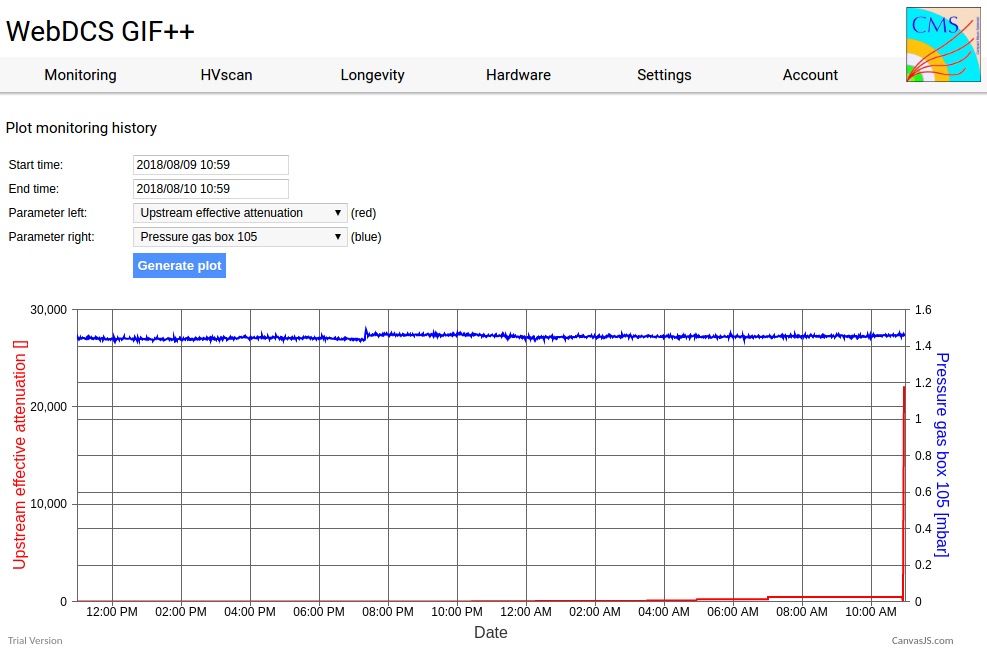
\includegraphics[width = \plotwidth]{fig/chapt5/DIP_monitoring_history.png}
		\caption{\label{fig:DIP-monitoring} DIP monitoring history accessed through the GIF++ WebDCS interface.}
	\end{figure}

	\subsection{Measurements performed during beam periods}
	\label{chapt5:ssec:beamperiods}
	
	As previously described, two types of measurements are performed on the chambers during beam periods. On the one hand, it is interesting to measure the efficiency of the RPCs with increasing voltage with different source absorber settings but on the other hand, it is important to correlate the efficiency information to the gamma rate seen by the chambers at the different voltages. The choice was made to separate efficiency measurements from rate measurements to better manage time and data volume. In both cases, TDC data recorded during so called \textit{HV scans} is divided into \textit{runs}, one for each high voltage point, whose data is stored into ROOT files. The TDC settings used during both these scans as well as the ROOT data structure are detailed in Section~\ref{app1:ssec:DataReader} of Appendix~\ref{app1}.
	
	The goal of both efficiency and rate scans is to measure the rate capability of the detectors but also to monitor any degradation of the performance due to ageing. This way, during test beam periods the efficiency and corresponding gamma background are measured to correlate the evolution of rate capability at different stages of irradiation. In the absence of other signs of ageing, a reduction of the rate capability could be related to an increase of the electrodes resistivity.
	
\newpage
	
		\subsubsection{Efficiency scans}
		\label{chapt5:sssec:effscan}
	
\begingroup\setlength{\intextsep}{0pt}\setlength{\columnsep}{15pt}
	
	\begin{wrapfigure}{O}{0.5\linewidth}
		\begin{subfigure}{\linewidth}
			\centering
			\includegraphics[width = \linewidth]{fig/chapt5/HV-Scan-Efficiency.pdf}
			\caption{\label{fig:efficiency-scan:A} Efficiency}
		\end{subfigure}
		\begin{subfigure}{\linewidth}
			\centering
			\includegraphics[width = \linewidth]{fig/chapt5/HV-Scan-ClS.pdf}\\
			\caption{\label{fig:efficiency-scan:B} Cluster size}
		\end{subfigure}
		\begin{subfigure}{\linewidth}
			\centering
			\includegraphics[width = \linewidth]{fig/chapt5/HV-Scan-Currents.pdf}
			\caption{\label{fig:efficiency-scan:C} Monitored currents}
		\end{subfigure}
		\caption{\label{fig:efficiency-scan} Example of results obtained during an efficiency scan performed with ABS 113 (4.6) during October 2018 testbeam period.}
	\end{wrapfigure}
	
	The HV scans performed to specifically measure the muon detection efficiency under different irradiation conditions follow a standardized procedure. Data using the DAQ is taken at the same 12 HV points for all chambers, ranging from \SI{9}{kV} to \SI{10.1}{kV} in steps of \SI{100}{V}. For each HV run, a minimum of 5000 muon beam triggers, provided by the coincidence of the three scintillators, is required in order to accumulate enough statistics for a reliable computation of the efficiency of the detectors. In addition to the four RPCs held on \texttt{T1}, two tracking RPCs installed on \texttt{T3} are kept at a fixed voltage of \SI{9,7}{kV} to provide the analysis software~\cite{GIFOffline} with beam position information to exclude off-track signals. The tracking RPCs are double gap detectors featuring \SI{2}{mm} HPL electrodes and \SI{2}{mm} gas gaps. They are prototypes built by the italian company \textit{General Tecnica} using a different production of HPL. Finally, the monitored currents and voltages are recorded in histograms along with the TDC data in a different ROOT file for each run.
	
	HV scans are taken for different source settings as the goal is to irradiate all the detectors with a minimal rate of \SIrate{600}. Usually, a full study of the performance of the detectors is performed with Source OFF, and then with nine absorber settings that attenuate the nominal gamma flux by factors from more than 200 to only 3, where settings with fully opened source are avoided with RPCs in test beam position. During the efficiency scans, the cluster size is also measured and the currents are monitored as can be seen in Figure~\ref{fig:efficiency-scan}.
	
\endgroup
	
		\subsubsection{Rate scans}
		\label{chapt5:sssec:ratescan}
		
	The background measurements are performed using a similar HV scan procedure as for the efficiency measurements. The HV scan in test beam periods is taken at fewer HV points compared to the efficiency scans as the region of interest is located around the knee and efficiency plateau of the detectors, i.e. these scans are performed only on six HV points ranging from \SI{9.5}{kV} to \SI{10}{kV}. The value of the rate at the operating voltage is then deduced from the efficiency scan through linear interpolation. A good estimation of the rate requires a long enough integrated time of the TDC data. The way data is collected, detailed in Appendix~\ref{app1}, makes the DAQ search for data stored in the TDC buffers prior to the trigger signal. The time window from which the data can be collected ranges from \SI{25}{ns} to more than \SI{50}{\mu s}. With the Cesium source delivering a constant gamma flux, it was decided that a total integrated time of \SI{0.2}{s} would be enough to have a reliable calculation of the gamma rate. This is achieved by taking 20,000 random trigger pulses delivered by a pulse generator at a frequency of \SI{300}{Hz} while extracting \SI{10}{\mu s} of data from the buffers for each trigger. An example of the data obtained during rate scans is showed in Figure~\ref{fig:rate-scan} in which the hit multiplicity at a single HV step of a scan, used to compute the rate per unit area, is showed together with the rates as computed at every HV steps.
	
	\begin{figure}[H]
    	\begin{subfigure}{0.5\linewidth}
			\centering
    		\includegraphics[width = \linewidth]{fig/chapt5/Hit_Multiplicity_RE2-2-NPD-BARC-9_A.pdf}
        	\caption{\label{fig:rate-scan:A} Hit multiplicity partition A}
    	\end{subfigure}
    	\begin{subfigure}{0.5\linewidth}
			\centering
    		\includegraphics[width = \linewidth]{fig/chapt5/Hit_Multiplicity_RE2-2-NPD-BARC-9_B.pdf}
        	\caption{\label{fig:rate-scan:B} Hit multiplicity partition B}
    	\end{subfigure}
    	\begin{subfigure}{0.5\linewidth}
			\centering
    		\includegraphics[width = \linewidth]{fig/chapt5/Hit_Multiplicity_RE2-2-NPD-BARC-9_C.pdf}
        	\caption{\label{fig:rate-scan:C} Hit multiplicity partition C}
    	\end{subfigure}
    	\begin{subfigure}{0.5\linewidth}
			\centering
    		\includegraphics[width = \linewidth]{fig/chapt5/Rate-Scan.pdf}
        	\caption{\label{fig:rate-scan:D} Rate scan}
    	\end{subfigure}
		\caption{\label{fig:rate-scan} Example of results obtained during an efficiency scan performed with ABS 113 (4.6) during October 2018 testbeam period. The hit multiplicity histograms \subref{fig:rate-scan:A}, \subref{fig:rate-scan:B} and \subref{fig:rate-scan:C} correspond to the fourth HV point of the scan at \SI{9800}{V}.}
	\end{figure}
		
	Separating the rate and efficiency measurements was motivated by the inconsistency of the muon beam provided in GIF++\footnote{During test beam periods, the delivery of the muon beam at the SPS North Area depends on the LHC program. As the SPS is used to feed the LHC with accelerated protons, the priority is given to the LHC. Other than the LHC, the delivery of muon beams can also be stopped due to maintenance or breakdown on the acceleration lane. This may translate into long periods with low intensity beams or even without any beam at all.}. Using periods without beam to measure rates with a good statistics allows for faster study programs. Moreover, the number of muons per beam spill depends strongly on the user setups placed upstream of the GIF++ and on the specific beam  optic magnet settings. Collecting 20,000 events could then take too long for the other users at the GIF++. Hence, efficiency scans are performed with lower statistics, and the time window from which the TDC data are extracted is strongly reduced (\si{400}{ns} for efficiency scans versus \SI{10}{\mu s} for rate scans) to keep the data size to its bare minimum.
	
		\subsubsection{Offline analysis and \acl{DQM}}
		\label{chapt5:sssec:DQM}

	\begin{figure}[H]
    	\begin{subfigure}{\linewidth}
			\centering
    		\includegraphics[width = .9\linewidth]{fig/chapt5/GIFpp-DQM-DAQ-fullpage.png}
        	\caption{\label{fig:DQM-DAQ:A}}
    	\end{subfigure}
    	\begin{subfigure}{\linewidth}
			\centering
    		\includegraphics[width = .9\linewidth]{fig/chapt5/GIFpp-DQM-DAQ.png}
        	\caption{\label{fig:DQM-DAQ:B}}
    	\end{subfigure}
		\caption{\label{fig:DQM-DAQ} Example of DQM page available on CMS RPC WebDCS at the GIF++: the histogram of the rate measured in one of the tracking chambers, namely \texttt{GT1\_20\_20-BKL\_JUL16\_4}, is selected and displayed above the page.}
	\end{figure}
		
	The data recorded during efficiency and rate scans always consists of two ROOT files per run, where each run corresponds to a certain HV point. One of the files contains the TDC data, a collection of hits and time stamps per active channel on the read-out of the RPCs, while the second is the CAEN main frame data, i.e. the detector currents and high voltages. The data are systematically analysed at the end of each scan using the Offline Analysis tool of GIF++, detailed in Appendix~\ref{app2}, that produces histograms such as hit, rate and time profiles, hit multiplicities, gamma cluster sizes or multiplicities for the DQM display of the WebDCS, as shown in Figure~\ref{fig:DQM-DAQ}. More histograms can be accessed through the ROOT browser included in the WebDCS, as shown in Figure~\ref{fig:DQM-ROOT}. Moreover, the analysis performed with the Offline tool provides final results for the rate scans. On the contrary, the algorithm for efficiency calculation is kept simple and approximative in the tool. Including tracking into the analysis requires manual adjustment for each individual scan as the positions of the trolleys with respect to each other may vary.

	\begin{figure}[H]
        \centering
		\includegraphics[width = \linewidth]{fig/chapt5/GIFpp-ROOT-browser.png}
		\caption{\label{fig:DQM-ROOT} Example of DQM ROOT Browser page available on CMS RPC WebDCS at the GIF++: the strip activity profile, defined as the rate profile normalized to the mean rate, in one of the tracking chambers, namely \texttt{GT1\_20\_20-BKL\_JUL16\_4}. Available ROOT files and histograms can be browsed thanks to the left panel showing the directory and files structures.}
	\end{figure}

	\subsection{Measurements performed during irradiation periods}
	\label{chapt5:ssec:irradiation}
	
	Even though test beam periods are stressful times as an extensive data taking program needs to be finalized in a short amount of time, the biggest amount of data actually comes from irradiation periods. Indeed, when \texttt{T1} is moved back to its ageing position in between each test beam periods, data is recorded at any time the source can be switched ON for irradiation. Other experiments in the area might prevent the source from staying open continuously. As an example, the time efficiency of irradiation of CMS RPC detectors in GIF++ is presented in Figure~\ref{fig:Irr-stat}.
	
	Several types of measurement are performed throughout the irradiation period. As long as the detectors are being irradiated, a monitoring of the currents is performed to evaluate the corresponding integrated charge over the total irradiation time. Moreover, in order to spot any signs of ageing, the gamma rates seen by the chambers at the chosen source absorber setting as well as the noise rates and dark currents are periodically measured. During irradiation periods this is looked at every week via HV scans performed at various source settings. The weekly scans involve both the irradiated but also the reference chambers, providing with a weekly monitoring of the evolution of the irradiated chambers noise, gamma rate and dark current. Measuring with all detectors at the same time also allows getting rid of potential systematics that might make the rates (noise or gamma) vary from one measurement to another. If such systematic effects occur, they will be observed in all detectors.
	
	Finally, the resistivity is measured periodically during the year, generally before or after test beam periods, by the use of Argon breakdown technique. The method consists in filling the detector volume with Argon instead of the CMS standard gas mixture and to increase the voltage while monitoring the current. Beyond an electric field of about \SI{1}{kV.mm^{-1}} at the GIF++ environmental conditions, Argon turns into a conductive plasma and does not offer electric resistance anymore. The monitoring of the currents beyond the breakdown voltage can then be used to calculate the resistivity of the electrode material.

	\begin{figure}[H]
        \centering
		\includegraphics[width = \linewidth]{fig/chapt5/GIFpp-irradiation-statistics.png}
		\caption{\label{fig:Irr-stat} Longevity data for chamber \texttt{RE2-2-NPD-BARC-9} in GIF++. For each month since July 2017, the integrated charge (in blue) as well as the time efficiency of irradiation (in gray) is reported.}
	\end{figure}
	
		\subsubsection{Longevity scans}
		\label{chapt5:sssec:longscan}
	
	The main activity of irradiation periods consists of the \textit{longevity scans} during which the currents of the irradiated chambers are continuously monitored. The two irradiated chambers, \texttt{RE2-2-NPD-BARC-09} and \texttt{RE4-2-CERN-166}, are both brought to a voltage of \SI{9.8}{kV} while the source flux can vary depending on the needs of the groups using the facility. The currents are monitored for each active gas volume as can be seen in Figure~\ref{fig:DQM-Longevity-Monitoring}. The integrated charge for each individual gas volume is computed by integrating through time the current density, current normalised to the surface area, flowing through each gap, as shown in Figure~\ref{fig:DQM-Longevity-Qint}.
	
\newpage
	
	\begin{figure}[H]
        \centering
		\includegraphics[width = \linewidth]{fig/chapt5/Longevity-scan-I-HVeff-vs-Time.png}
		\caption{\label{fig:DQM-Longevity-Monitoring} Example of a longevity scan monitoring page available on CMS RPC WebDCS at the GIF++: the current and effective voltage, as well as environmental parameters, are monitored for the bottom gap of chamber \texttt{RE2-2-NPD-BARC-9}. The decrease of current is related to a decrease of the voltage due to the daily rate scan procedure or to periods during which the source was turned OFF.}
	\end{figure}
	
	\begin{figure}[H]
        \centering
		\includegraphics[width = \linewidth]{fig/chapt5/Longevity-scan-Qint-vs-Time.png}
		\caption{\label{fig:DQM-Longevity-Qint} Example of a longevity scan summary page available on CMS RPC WebDCS at the GIF++: the integrated charge is computed for the bottom gap of chamber \texttt{RE2-2-NPD-BARC-9}.}
	\end{figure}
	
	Finally, at the end of each longevity scan each gap contribution is translated into the mean chamber integrated charge. The integrated charge accumulated in each chamber is used to update the summary plots providing the collaboration with official results to be spread as can be seen from Figure~\ref{fig:Longevity}. The translation from individual gap currents to total integrated charge in the chamber is done using Equation~\ref{eq:Qint}, where the equation to compute the monitored current density already mentioned in Section~\ref{chapt5:ssec:resultsGIF} is recalled.
	
	\begin{equation}
	\label{eq:Qint}
		\begin{aligned}
	J_{mon} &= \frac{I_{mon}^{TW}+I_{mon}^{TN}}{A_{TW}+A_{TN}} + \frac{I_{mon}^B}{A_B}\\
	Q_{int} &= \int_{t_i}^{t_f} J_{mon}dt
		\end{aligned}
	\end{equation}
	
	\begin{figure}[H]
    	\begin{subfigure}{0.5\linewidth}
			\centering
    		\includegraphics[width = \linewidth]{fig/chapt5/GIFpp-Longevity-monitoring-TW.pdf}
        	\caption{\label{fig:Longevity:A}}
    	\end{subfigure}
    	\begin{subfigure}{0.5\linewidth}
			\centering
    		\includegraphics[width = \linewidth]{fig/chapt5/GIFpp-Longevity-monitoring-TN.pdf}
        	\caption{\label{fig:Longevity:B}}
    	\end{subfigure}
    	\begin{subfigure}{0.5\linewidth}
			\centering
    		\includegraphics[width = \linewidth]{fig/chapt5/GIFpp-Longevity-monitoring-BOT.pdf}
        	\caption{\label{fig:Longevity:C}}
    	\end{subfigure}
    	\begin{subfigure}{0.5\linewidth}
			\centering
    		\includegraphics[width = \linewidth]{fig/chapt5/GIFpp-Longevity-int-charge.pdf}
        	\caption{\label{fig:Longevity:D}}
    	\end{subfigure}
		\caption{\label{fig:Longevity} Example of current monitoring summary (top wide~\subref{fig:Longevity:A}, top narrow~\subref{fig:Longevity:B} and bottom~\subref{fig:Longevity:C} gap currents) and of corresponding integrated charge~\subref{fig:Longevity:D} of chamber \texttt{RE2-2-NPD-BARC-09}.}
	\end{figure}
\vfill
	
\newpage
	
		\subsubsection{Daily rate monitoring scans}
		\label{chapt5:sssec:dailyratescan}
	
	Every night during longevity scans, the setup performs \textit{daily rate scans}. These scans aim at keeping track of the gamma rate measured in the irradiated RPCs during longevity scans, but are also used to measure the noise rate at standby voltage for each gap. The procedure for these HV scans consist of nine runs for which 50,000 random triggers are accumulated, corresponding to \SI{0.5}{s} of total integrated time.
	
	\begin{itemize}
		\item[1-] All gaps are first left at the irradiation voltage of \SI{9.8}{kV} to measure the gamma rate.
		\item[2-] Then all gaps are brought to the standby voltage of \SI{6.5}{kV} to measure the noise rate of the full detectors.
		\item[3-] Both top gaps (TW and TN) are brought to a voltage equivalent to an OFF status, i.e. \SI{1}{kV} so that the noise contribution of only the bottom gap at standby voltage can be measured.
		\item[4-] The bottom gaps are ramped up toward the working voltage of \SI{9.8}{kV} to measure their contribution to the gamma rate estimation.
		\item[5-8] The steps 3 and 4 are repeated on TN and then on TW, keeping the bottom and the top gap which is not of interest at a voltage of \SI{1}{kV}. This way, the individual contribution to the noise and gamma rates are known.
		\item[9-] Both TW and TN are brought to working voltage while the bottom gap is left at \SI{1}{kV} to measure the gamma rate for the full top layer at once.
	\end{itemize}
	
	Finally, the voltages of all gaps are brought back to working voltage for the longevity program to continue until the next daily scan. These scans are responsible for the drop of voltages and currents observed in Figure~\ref{fig:DQM-Longevity-Monitoring}. The procedure previously described is highlighted in Figure~\ref{fig:Daily-Scan-Proc}. 
	
	Similarly to the efficiency and rate scans taken during test beam periods, the data is here stored in two separate ROOT files for the TDC and CAEN data for each run. At the same time, the currents are still monitored by the longevity scan and saved into the GIF++ database for an easy evaluation of the currents to the integrated charge. The Offline Analysis tool then provides the DQM page with histograms, and daily values can be compiled into long term monitoring plots to study the variations of rate and current with increasing integrated charge, as presented in Figure~\ref{fig:rate-I-monitor}. The variations of the rate and current are correlated and correspond mainly to change of source irradiation, gas flow, gas humidity, or environmental conditions. The rates on every single read-out channel are also tracked to control their activity with increasing integrated charge and, this way, understand the appearance of hot spots through noisy channels, as shown in Figure~\ref{fig:stripactivity}. The activity of a strip is defined as the rate of the individual channel normalized to the mean rate measured in the corresponding read-out partition.

	\begin{figure}[H]
    	\begin{subfigure}{\linewidth}
			\centering
    		\includegraphics[width = .9\linewidth]{fig/chapt5/Daily-rate-scan-BOT.png}
        	\caption{\label{fig:Daily-Scan-Proc:A} Bottom gap}
    	\end{subfigure}
    	\begin{subfigure}{\linewidth}
			\centering
    		\includegraphics[width = .9\linewidth]{fig/chapt5/Daily-rate-scan-TN.png}
        	\caption{\label{fig:Daily-Scan-Proc:B} Top narrow gap}
    	\end{subfigure}
    	\begin{subfigure}{\linewidth}
			\centering
    		\includegraphics[width = .9\linewidth]{fig/chapt5/Daily-rate-scan-TW.png}
        	\caption{\label{fig:Daily-Scan-Proc:C} Top wide gap}
    	\end{subfigure}
		\caption{\label{fig:Daily-Scan-Proc} Example of daily scan procedure of chamber \texttt{RE2-2-NPD-BARC-09} with highlighted runs on the CMS RPC WebDCS at the GIF++.}
	\end{figure}
	
	\begin{figure}[H]
    	\begin{subfigure}{0.5\linewidth}
			\centering
    		\includegraphics[width = 0.5\plotwidth]{fig/chapt5/GIFpp-Rate-vs-Q.pdf}
        	\caption{\label{fig:rate-I-monitor:A}}
    	\end{subfigure}
    	\begin{subfigure}{0.5\linewidth}
			\centering
    		\includegraphics[width = 0.5\plotwidth]{fig/chapt5/GIFpp-I-vs-Q.pdf}
        	\caption{\label{fig:rate-I-monitor:B}}
    	\end{subfigure}
		\caption{\label{fig:rate-I-monitor} Example of rate~\subref{fig:rate-I-monitor:A} and current~\subref{fig:rate-I-monitor:B} monitoring of chamber \texttt{RE2-2-NPD-BARC-09} at working voltage in double gap mode (step 1) with increasing integrated charge.}
	\end{figure}

	\begin{figure}[H]
        \centering
		\includegraphics[width = \linewidth]{fig/chapt5/GIFpp-Strip-Activity.pdf}
		\caption{\label{fig:stripactivity} Example of strip activity of chamber \texttt{RE2-2-NPD-BARC-09} monitored over time.}
	\end{figure}
	
		\subsubsection{Weekly noise monitoring scans}
		\label{chapt5:sssec:noisescan}
		
	Once a week, the source is turned OFF to make a noise scan for the CMS RPC. This HV scan is composed of six runs for which 25,000 random triggers are accumulated. The first run is taken at standby voltage and the second one at \SI{8}{kV}. The next five runs are taken at voltages ranging from 9.4 to \SI{9.8}{kV} in order to access for both type of chambers, RE2 and RE4, in the voltage region where the efficiency rises and reaches its plateau. The whole procedure is shown in Figure~\ref{fig:weekly-noise}. On the occasion of this scan, the ongoing longevity scan is stopped. A new one will be started once the weekly scans are over.
	
	\begin{figure}[H]
    	\begin{subfigure}{0.5\linewidth}
			\centering
    		\includegraphics[width = \linewidth]{fig/chapt5/Weekly-noise-Scan-Currents.pdf}
        	\caption{\label{fig:weekly-noise:A}}
    	\end{subfigure}
    	\begin{subfigure}{0.5\linewidth}
			\centering
    		\includegraphics[width = \linewidth]{fig/chapt5/Weekly-noise-Scan-Rates.pdf}
        	\caption{\label{fig:weekly-noise:B}}
    	\end{subfigure}
		\caption{\label{fig:weekly-noise} Example of rates~\subref{fig:rate-I-monitor:A} and currents~\subref{fig:rate-I-monitor:B} of irradiated chamber \texttt{RE4-2-CERN-166} and reference chamber \texttt{RE4-2-CERN-165} measured during a weekly noise scan.}
	\end{figure}
	
		\subsubsection{Weekly source scans}
		\label{chapt5:sssec:sourcescan}
		
	Directly following the weekly noise scans, HV rate scans are organised at different source settings (usually ABS 6.8, 4.6 and 3.3). The procedure of these HV scans consists of nine runs for which 25,000 random triggers are accumulated. The first run is taken at standby voltage while the next eight runs are taken at voltages ranging from 9.4 to \SI{10.1}{kV}. They aim at measuring the gamma rate to which the chambers are subjected and the related currents. The whole procedure is shown in Figure~\ref{fig:weekly-source}.
	
	\begin{figure}[H]
    	\begin{subfigure}{0.5\linewidth}
			\centering
    		\includegraphics[width = \linewidth]{fig/chapt5/Weekly-source-Scan-Currents.pdf}
        	\caption{\label{fig:weekly-source:A}}
    	\end{subfigure}
    	\begin{subfigure}{0.5\linewidth}
			\centering
    		\includegraphics[width = \linewidth]{fig/chapt5/Weekly-source-Scan-Rates.pdf}
        	\caption{\label{fig:weekly-source:B}}
    	\end{subfigure}
		\caption{\label{fig:weekly-source} Example of rates~\subref{fig:rate-I-monitor:A} and currents~\subref{fig:rate-I-monitor:B} of irradiated chamber \texttt{RE4-2-CERN-166} and reference chamber \texttt{RE4-2-CERN-165} measured during a weekly source scan. The data were measured with ABS 123 (6.9).}
	\end{figure}
	
		\subsubsection{Weekly current scans}
		\label{chapt5:sssec:currentscan}
	
\begingroup\setlength{\intextsep}{0pt}\setlength{\columnsep}{15pt}
	
	\begin{wrapfigure}{O}{0.55\linewidth}
		\centering
    	\includegraphics[width = \linewidth]{fig/chapt5/Weekly-current-Scan.pdf}
		\caption{\label{fig:weekly-current} Example of currents of irradiated chamber \texttt{RE4-2-CERN-166} and reference chamber \texttt{RE4-2-CERN-165} measured during a weekly current scan.}
	\end{wrapfigure}
		
	The previously detailed daily rate scans, but also the weekly noise and source scans are interesting tools to look at an increase of noise rates and dark currents or at a loss of rate capability. They could point to an increase of surface resistivity of the electrodes through the absorption of hydrofluoric acid. Nevertheless, periodically measuring the currents on wider high voltage ranges allows to have access to the ohmic part of the current driven by the detectors related to the electrodes resistance. This is why precise current scans, consisting only in measuring the current driven through the four detectors, are performed each week. The scan procedure includes measurements at 131 high voltage points in between \SI{500}{V} and \SI{10}{kV}, in steps of \SI{100}{V} until the standby voltage of \SI{6.5}{kV} is reached and then in steps of \SI{50}{V}. At low voltage, the current rise is slow and is only driven by the resistance of the detector electrode and thus increases linearly. It is referred to as the \textit{ohmic current} as opposed to the \textit{physics current} corresponding to the voltage region where charge multiplication starts to occur . A fit on the ohmic current range gives access to the resistance of the \textit{'electrodes/gas'} system. If any variation of the electrode resistance occurs, the global resistance will increase and so will the current. Technically, these scans will record a ROOT file per HV step that will have the same format as the CAEN ROOT file saved during other HV scans. The data is also analysed using the Offline Analysis tool to provide with DQM histograms as well as standardized $I/V$ tables.
	
\endgroup
	
	\subsection{Extraction and monitoring of the resistivity}
	\label{chapt5:ssec:resistivity}
	
\begingroup\setlength{\intextsep}{0pt}\setlength{\columnsep}{15pt}
	
	\begin{wrapfigure}{O}{0.5\linewidth}
		\centering
    	\includegraphics[width = \linewidth]{fig/chapt5/Argon-Scan.pdf}
		\caption{\label{fig:argon-scan} Example of currents of irradiated chamber \texttt{RE2-2-NPD-BARC-09} measured during an argon scan. The resistance is extracted from the linear fit and the resistivity is computed using Equation~\ref{eq:resistivity}.}
	\end{wrapfigure}
	
	A critical parameter to monitor is the resistivity of the electrodes. Its variation would impact the rate capability of the RPC. An increase of the resistivity with increased irradiation is expected. In the first place, the measurement of the resistivity of the electrodes is done using the so called \textit{Argon scans}. Such tests are performed regularly before or after test beam periods through high voltage scans of the detectors operated with pure Argon. The electric field strength at which Argon breaks down being well known, the current beyond the breakdown voltage is monitored. Assuming a relation $I_{mon} = HV_{eff}/R_{elec}$ beyond the breakdown voltage,  the resistance of the couple of electrodes $R_{elec}$ is extracted as can be seen from Figure~\ref{fig:argon-scan}. The resistivity is then deduced by using Formula~\ref{eq:resistivity} where $S$ is the surface area of the gap and $l$ the thickness of a single electrode.
	
\endgroup
	
	\begin{equation}
	\label{eq:resistivity}
	\rho = R \times \frac{S}{2 \times l}
	\end{equation}
	
	There exist other ways to access a quantity directly related to the resistivity. During the testbeam periods, the efficiency of the detectors is measured with both source OFF and source ON with high irradiation. The shift of voltage introduced by an irradiation is directly linked to the rate capability of the detector and hence to the resistivity of the electrodes. By comparing the efficiency curves observed with source ON and OFF during a single testbeam, it is possible to access the local mean resistance of the detector during a testbeam period. This value can be compared to the resistivity directly measured using the argon scans. It also provides a tool to compare different testbeam results by getting rid of the bias introduced by the fluctuation of the resistivity through time. The mean resistance is computed as in Formula~\ref{eq:resistance-shift}.
	
	\begin{equation}
	\label{eq:resistance-shift}
	R = \frac{\Delta HV}{\Delta I} = \frac{HV^{ON} - HV^{OFF}}{I^{ON} - I^{OFF}}
	\end{equation}
	
	\begin{figure}[H]
    	\begin{subfigure}{\linewidth}
			\centering
    		\includegraphics[width = 0.5\linewidth]{fig/chapt5/HVeff-Graph-BARC-9.pdf}
        	\caption{\label{fig:october-sig:A} $\epsilon(HV_{eff})$}
    	\end{subfigure}
    	\begin{subfigure}{0.5\linewidth}
			\centering
    		\includegraphics[width = \linewidth]{fig/chapt5/Imon-Graph-BARC-9-BOT.pdf}
        	\caption{\label{fig:october-sig:B} $I_{mon}^{BOT}(HV_{eff})$}
    	\end{subfigure}
    	\begin{subfigure}{0.5\linewidth}
			\centering
    		\includegraphics[width = \linewidth]{fig/chapt5/Imon-Graph-BARC-9-TN.pdf}
        	\caption{\label{fig:october-sig:C} $I_{mon}^{TN}(HV_{eff})$}
    	\end{subfigure}
		\caption{\label{fig:october-sig} Efficiency~\subref{fig:october-sig:A} and monitored currents of the bottom~\subref{fig:october-sig:B} and top narrow~\subref{fig:october-sig:C} gaps as a function of the effective voltage of chamber \texttt{RE2-2-NPD-BARC-09} during October 2018 testbeam period.}
	\end{figure}
	
	It is important to note that the result provided by using this method will only concern the resistance of the detector under the beam, including the little contribution of the resistance of the gas volume itself. The translation to the resistivity of the electrodes is not straight forward even though the result falls in the same order of magnitude. Also, the quality of the resistance extraction depends on which level of irradiation is available in the data. During October 2018 testbeam period, HV scans were done on partition C of the RPCs (bottom and top narrow gas gaps) with source OFF and with eight diffent ABS values: ABS 313 (464), ABS 311 (100), ABS 213 (46.4), ABS 212 (21.5), ABS 211 (10), ABS 123 (6.9), ABS 113 (4.6) and ABS 122 (3.2). T1 was placed close to the bunker upstream wall at a distace of \SI{5.6}{m} from the source. This position corresponds to a gamma current of the order of \Sci{5}{5}\siflux with source fully open.
	
	In a first step, the efficiency sigmoids as well as the bottom and top narrow gaps' monitored current as a function of the effective voltage were retrieved as can be seen from Figure~\ref{fig:october-sig}. The goal is to compute the value of the effective voltage at the knee $HV_{knee}$ of the sigmoids. The knee where $\epsilon = 0.95 \times \epsilon_{max}$ would be the best location to extract the value of the resistivity. At this point, the performance of the detectors is stable and a little variation of voltage does not have a large effect on the efficiency. The effective voltage at the knee is given by Formula~\ref{eq:knee}.
	
	\begin{equation}
	\label{eq:knee}
	HV_{knee} = HV_{50} + \frac{ln(19)}{\lambda}
	\end{equation}
	
	The monitored current at the knee $I_{knee}^{G}$ for each gap $G$ is then computed by extrapolating from the monitored currents value located around $HV_{knee}$ as in Formula~\ref{eq:extrapolation} where $I_{\downarrow}^{G}$ and $HV_{\downarrow}^{G}$ are the monitored current and the effective voltage at the voltage point bellow the knee and $I_{\uparrow}^{G}$ and $HV_{\uparrow}^{G}$ are the monitored current and the effective voltage above the knee.
	
	\begin{equation}
	\label{eq:extrapolation}
	I_{knee}^{G} = I_{\downarrow}^{G} + (I_{\uparrow}^{G} + I_{\downarrow}^{G})\times\frac{HV_{knee}-HV_{\downarrow}^{G}}{HV_{\uparrow}^{G} - HV_{\downarrow}^{G}}
	\end{equation}
	
	Once the values of the monitored currents are known at the knee, the mean current flowing through the gaps at the level of the studied partition $P$ can be computed. First of all, the currents at knee of the gaps in the beam line is normalised to the area of the gap active area seen by the local read-out partition $S^{G,P}$. Then the mean current at knee $\overline{I}_{knee}^{P}$ is computed by ponderating the local currents $I_{knee}^{G,P}$ of each gap by their respective active area in the partition.
	
	\begin{equation}
	\label{eq:meanI}
		\begin{aligned}
	I_{knee}^{G,P} &= \frac{I_{knee}^{G} \times S^{G,P}}{S^{G}}\\
	\overline{I}_{knee}^{P} &= \frac{I_{knee}^{1,P}\times S^{1,P} + I_{knee}^{2,P}\times S^{2,P}}{S^{1,P} + S^{2,P}}
		\end{aligned}
	\end{equation}
	
	The variation of effective voltage and mean monitored current at the knee in between the Source OFF and ON scans can then be obtained. The local resistivity of the detector can finally be calculated combining Formula~\ref{eq:resistivity} and Formula~\ref{eq:resistance-shift}. This process is performed for every scan of each approved test beam period as can be seen in Figure~\ref{fig:Resistivity-Fit}. Finally, the most probable resistivity during the test beam period is obtained thanks to a constant fit. The value of the mean partition resistivity displayed in Figure~\ref{fig:Resistivity-Fit} is of the same order than what would be expected for CMS RPCs.
	
	Later, the value extracted from this method will be used to compare the efficiency sigmoids of the different testbeam periods. During the operation of the detector without irradiation, the voltage drop across the detector almost only consists in a voltage drop across the gas volume. As the electrodes behave approximately as charged capacitors, there is only a negligible voltage drop across their volume. The charge of the electrodes is only affected locally by the charge carriers freed by avalanches in the gas volume. Nevertheless, under irradiation, the conversion of photons is uniform throughout the electrodes' volume and charge recombination happens everywhere at the same time making it impossible for the electrodes to stay charged. Hence, a significant part of the voltage drop appears across the electrodes, explaining the usual voltage shift observed in the performance of irradiated RPCs. The data comparison will then be done using the gas voltage drop $HV_{gas}$ obtained by correcting the effective voltage $HV_{eff}$ thanks to Formula~\ref{eq:HVgas} in which $R$ is the resistance computed at the knee using Formula~\ref{eq:resistance-shift} in the RPC partition of interest and $\overline{I}$ is the mean current in this partition at each voltage step.
	
	\begin{equation}
	\label{eq:HVgas}
		HV_{gas} = HV_{eff} - R\times\overline{I}
	\end{equation}
	
	\begin{figure}[H]
    	\begin{subfigure}{0.5\linewidth}
			\centering
    		\includegraphics[width = \linewidth]{fig/chapt5/Resistivity-vs-Rate-BARC-8.pdf}
        	\caption{\label{fig:Resistivity-Fit:A}}
    	\end{subfigure}
    	\begin{subfigure}{0.5\linewidth}
			\centering
    		\includegraphics[width = \linewidth]{fig/chapt5/Resistivity-vs-Rate-BARC-9.pdf}
        	\caption{\label{fig:Resistivity-Fit:B}}
    	\end{subfigure}
    	\begin{subfigure}{0.5\linewidth}
			\centering
    		\includegraphics[width = \linewidth]{fig/chapt5/Resistivity-vs-Rate-CERN-165.pdf}
        	\caption{\label{fig:Resistivity-Fit:C}}
    	\end{subfigure}
    	\begin{subfigure}{0.5\linewidth}
			\centering
    		\includegraphics[width = \linewidth]{fig/chapt5/Resistivity-vs-Rate-CERN-166.pdf}
        	\caption{\label{fig:Resistivity-Fit:D}}
    	\end{subfigure}
		\caption{\label{fig:Resistivity-Fit} Resistivity extraction for all approved test beam periods for the reference RE2/2~\subref{fig:Resistivity-Fit:A} and RE4/2~\subref{fig:Resistivity-Fit:C} chambers and the irradiated RE2/2~\subref{fig:Resistivity-Fit:B} and RE4/2~\subref{fig:Resistivity-Fit:D} chambers.}
	\end{figure}
	
\newpage
	
	\subsection{Results and discussions}
	\label{chapt5:ssec:resultsGIFpp}
	
\begingroup\setlength{\intextsep}{0pt}\setlength{\columnsep}{15pt}
	
	\begin{wrapfigure}{O}{0.6\linewidth}
        \centering
		\includegraphics[width = \linewidth]{fig/chapt5/GIFpp-Qint.pdf}
		\caption{\label{fig:GIFppQint} Total integrated charge in the irradiated RPCs, \texttt{RE2-2-NPD-BARC-9} and \texttt{RE4-2-CERN-165}, in July 2019. The irradiation of the RE2 chamber started early July 2016 while the RE4 chamber couldn't be irradiated before end of November 2016.}
	\end{wrapfigure}
    
    Since 2015, CMS RPCs have been irradiated at the GIF++ with the goal to reach a total integrated charge per irradiated detector of \SI{0.84}{C/cm^2} while certifying the detectors to a single hit rate capability of \SIrate{600}. At the time of writing, the RE2 and RE4 chambers were exposed to 74 and 40\% of their total irradiation program respectively, as shown in Figure~\ref{fig:GIFppQint}. According to Figure~\ref{fig:GIFppQint-Extrapol}, a few years of irradiation are expected before reaching the end of the longevity study for both types of detectors and before reaching a final answer on whether the present CMS RPC system will be able to live through HL-LHC or not. The charge accumulation of the RE2 detector is faster than which of the RE4 and is expected to end within a year. In the case of the RE4 RPC, the irradiation would go on for more than two years at the current charge accumulation rate. This time would be reduced after the end of the logevity study of the RE2 by placing the trolley hosting the detectors closer to the source.
    
\endgroup
	
\begingroup\setlength{\intextsep}{0pt}\setlength{\columnsep}{15pt}
	
	\begin{wrapfigure}{O}{0.6\linewidth}
        \centering
		\includegraphics[width = \linewidth]{fig/chapt5/Qint-vs-Time-Extrapolation.pdf}
		\caption{\label{fig:GIFppQint-Extrapol} Linear projection of the time necessary to finish the longevity program on the RE2 and RE4 detectors at the GIF++.}
	\end{wrapfigure}
	
	Throughout the longevity program, great care was put into monitoring the detector characteristics. While presenting the results, current densities expressed in \si{\mu A/cm^2} will be showed in the place of currents. In the first part of the discussion the current densities will be refered to as "dark current". Also, the data of the reference detectors will be displayed with increasing integrated charge. This integrated charge will always refer to the integrated charge of the irradiated detectors.
	
	Using the data collected during the weekly noise scans performed on all four RPCs, the dark currents are monitored. Two voltage of interest are being compared through time. The first value of interest was chosen at a \textit{STANDBY} voltage of \SI{6500}{V} where no multiplication process happens. This is done to follow the variations of the ohmic component of the current. The monitored dark current in STANDBY are shown in Figure~\ref{fig:GIFpp-Ohmic-mon}. At the time of writing, the ohmic currents for all detectors are stable. Both RE4 detectors appear to follow the same trend while the ohmic current of the irradiated RE2 detector has increased a little. Nevertheless, this increase is only of 10 to \SI{20}{pA/cm^2} and a similar behaviour can be observed for both RE4 detectors. There is no reason to associate the increase in ohmic current with the irradiation.
    
\endgroup

	\begin{figure}[H]
    	\begin{subfigure}{0.5\linewidth}
    		\centering
			\includegraphics[width = \linewidth]{fig/chapt5/RE2-2-Dark-Current-vs-Time-6500.png}
        	\caption{\label{fig:GIFpp-Ohmic-mon:A}}
    	\end{subfigure}
    	\begin{subfigure}{0.5\linewidth}
			\centering
    		\includegraphics[width = \linewidth]{fig/chapt5/RE4-2-Dark-Current-vs-Time-6500.png}
        	\caption{\label{fig:GIFpp-Ohmic-mon:B}}
    	\end{subfigure}
		\caption{\label{fig:GIFpp-Ohmic-mon} Monitoring of the ohmic component of the dark current with increasing integrated charge at a voltage of \SI{6500}{V} of the RE2-2~\subref{fig:GIFpp-Ohmic-mon:A} and RE4-2~\subref{fig:GIFpp-Ohmic-mon:B} detectors installed at the GIF++.}
	\end{figure}
	
	The second value of interest is located in the gain region near the working point at a voltage of \SI{9600}{V} for the RE2 detectors and of \SI{9500}{V} for the RE4 ones. Monitoring the multiplication region allows to spot the appearance of hot spots accross the detectors' areas. A local damage to the electrode could result in an increase of local discharges and an overal increase of the current drawn by the detector which would show in the monitored values. Near the working voltage, in addition to the current densities, the noise rate per unit are monitored as can be seen in Figure~\ref{fig:GIFpp-Dark-rate-mon}. In the case of the RE2 detectors, the dark currents and noise rate stay stable since the begining of the irradiation program. The variability of the dark current of the irradiated chamber is higher than the one of the reference chamber but seem to always come back between 0.1 and \SI{0.15}{nA/cm^2}. Concerning the RE4 detectors, both chambers are very stable up to an irradiation of \SI{150}{mC/cm^2}. Even though the noise rate of the reference chamber seem to fluctuate a lot between 0.5 and \SI{3.5}{Hz/cm^2} before this value, the monitoring of the noise rate per unit area following this early range as well as the very stable dark current would suggest that the chamber was in fact suffering from a bad grounding. Indeed, beyond \SI{150}{mC/cm^2}, the noise rate suddenly stabilizes between 0.1 and \SI{0.2}{Hz/cm^2} while the dark current increases very slightly to \SI{50}{pA/cm^2}. On the contrary, the irradiated chamber which was very stable under \SI{150}{mC/cm^2}, sees its dark current and its noise rate increase and fluctuate with a similar shape. The noise rate is still within the requirements of CMS. Indeed, an upper threshold of \SI{1}{Hz/cm^2} was considered to be good enough to prevent fake events due to noise. Reguarding the dark current, so far the highest peak, reached a little higher than \SI{0.4}{nA/cm^2} and have since droped to \SI{0.2}{nA/cm^2}. During \textit{source scans} at gamma rates per unit area usually above \SI{400}{Hz/cm^2}, the current densities are of the order of \SI{10}{nA/cm^2}, almost two orders of magnitude larger than the dark current. Nevertheless, both the noise rate and dark current have almost gained an order of magnitude at their highest monitored values and will need to be carefully followed at higher values of integrated charge.

	\begin{figure}[H]
    	\begin{subfigure}{0.5\linewidth}
    		\centering
			\includegraphics[width = \linewidth]{fig/chapt5/RE2-2-Dark-Current-vs-Time-9600.png}
        	\caption{\label{fig:GIFpp-Dark-rate-mon:A}}
    	\end{subfigure}
    	\begin{subfigure}{0.5\linewidth}
			\centering
    		\includegraphics[width = \linewidth]{fig/chapt5/RE4-2-Dark-Current-vs-Time-9500.png}
        	\caption{\label{fig:GIFpp-Dark-rate-mon:B}}
    	\end{subfigure}
    	\begin{subfigure}{0.5\linewidth}
    		\centering
			\includegraphics[width = \linewidth]{fig/chapt5/RE2-2-Noise-rate-vs-Time-9600.png}
        	\caption{\label{fig:GIFpp-Dark-rate-mon:C}}
    	\end{subfigure}
    	\begin{subfigure}{0.5\linewidth}
			\centering
    		\includegraphics[width = \linewidth]{fig/chapt5/RE4-2-Noise-rate-vs-Time-9500.png}
        	\caption{\label{fig:GIFpp-Dark-rate-mon:D}}
    	\end{subfigure}
		\caption{\label{fig:GIFpp-Dark-rate-mon} Monitoring of the physics component of the dark current and of the noise rate per unit area with increasing integrated charge at a voltage of \SI{9600}{V} for the RE2-2 detectors~\subref{fig:GIFpp-Dark-rate-mon:A} and~\subref{fig:GIFpp-Dark-rate-mon:C} and at a voltage of \SI{9500}{V} for the RE4-2 detectors~\subref{fig:GIFpp-Dark-rate-mon:B} and~\subref{fig:GIFpp-Dark-rate-mon:D} installed at the GIF++.}
	\end{figure}
	
	The same exercise is done using the data collected during the weekly source scans. The monitoring of the current densities and of the gamma rate per unit area is showed in Figure~\ref{fig:GIFpp-Source-mon}. The reported measurements are always performed with the same source conditions corresponding to an irradiation attenuated by a factor 6.9. The increase in dark current of the irradiated RE4 chamber don't have any visible effect when the source irradiates the detectors. No signs of ageing due to irradiation is yet to be seen for both the RE2 and RE4 detectors. The current densities and gamma rates of all four detectors evolve following the same phases of increase and decrease, as confirmed by Figure~\ref{fig:GIFpp-J_R_correlation}.

	\begin{figure}[H]
    	\begin{subfigure}{0.5\linewidth}
    		\centering
			\includegraphics[width = \linewidth]{fig/chapt5/RE2-2-Source-Current-vs-Time-9600.png}
        	\caption{\label{fig:GIFpp-Source-mon:A}}
    	\end{subfigure}
    	\begin{subfigure}{0.5\linewidth}
			\centering
    		\includegraphics[width = \linewidth]{fig/chapt5/RE4-2-Source-Current-vs-Time-9500.png}
        	\caption{\label{fig:GIFpp-Source-mon:B}}
    	\end{subfigure}
    	\begin{subfigure}{0.5\linewidth}
    		\centering
			\includegraphics[width = \linewidth]{fig/chapt5/RE2-2-Source-Rate-vs-Time-9600.png}
        	\caption{\label{fig:GIFpp-Source-mon:C}}
    	\end{subfigure}
    	\begin{subfigure}{0.5\linewidth}
			\centering
    		\includegraphics[width = \linewidth]{fig/chapt5/RE4-2-Source-Rate-vs-Time-9500.png}
        	\caption{\label{fig:GIFpp-Source-mon:D}}
    	\end{subfigure}
		\caption{\label{fig:GIFpp-Source-mon} Monitoring of the current density and of the gamma rate per unit area under irradiation with increasing integrated charge at a voltage of \SI{9600}{V} for the RE2-2 detectors~\subref{fig:GIFpp-Source-mon:A} and~\subref{fig:GIFpp-Source-mon:C} and at a voltage of \SI{9500}{V} for the RE4-2 detectors~\subref{fig:GIFpp-Source-mon:B} and~\subref{fig:GIFpp-Source-mon:D} installed at the GIF++. The source irradiation is attenuated by a factor 6.9.}
	\end{figure}
	
	The use of \acf{PCA}~\cite{PCA} reveals that the study of the correlations between the current densities and the gamma rates can be reduced to a single dimension. To perform the PCA, the algorithm used normalises each variable to get a mean value of 0 and a variance of 1 resulting in the study of the variance. The associated \textit{Scree} plot~\cite{SCREE} showed in Figure~\ref{fig:GIFpp-J_R_correlation:B} indicates for each of the components of the PCA, the eigen values of the covariance matrix. In this case, the eigen values have been normalised to express the percentage of variance explained by each component. More than 93\% of the data variation can be explained using a simple linear composition of the current density and of the gamma rate. It is expected as the current density and gamma rate are two side of the same physical process. Any deviation would mean that other processes than the convertion of photons in the electrode material take place.

	\begin{figure}[H]
    	\begin{subfigure}{0.5\linewidth}
    		\centering
			\includegraphics[width = \linewidth]{fig/chapt5/Gamma_rate-vs-Current_density.pdf}
        	\caption{\label{fig:GIFpp-J_R_correlation:A}}
    	\end{subfigure}
    	\begin{subfigure}{0.5\linewidth}
			\centering
    		\includegraphics[width = \linewidth]{fig/chapt5/Scree_plot_J-vs-R.pdf}
        	\caption{\label{fig:GIFpp-J_R_correlation:B}}
    	\end{subfigure}
		\caption{\label{fig:GIFpp-J_R_correlation} \subref{fig:GIFpp-J_R_correlation:A} Gamma rates as a function of the corresponding current densities. \subref{fig:GIFpp-J_R_correlation:B} Scree plot obtained at the output of PCAs performed on each set of current densities and corresponding gamma rates.}
	\end{figure}
	
	The fluctuations observed on Figure~\ref{fig:GIFpp-Source-mon} may arise due to different factors such as the environmental conditions (gas temperature, gas relative humidity, environmental pressure) or the presence of other experiments between the source. The distance from the source and the trolley, and the gamma current at which the detectors are irradiated during the ageing procedure are kept as consistent as possible and should not contribute to the fluctuations in current density and gamma rate. In order to have a better understanding, the monitoring of the environmental parameters, i.e. the gas relative humity and temperature both at the supply and at the exhaust of the trolley together with the humidity and temperature inside of the bunker and the environmental pressure, is showed in Figures~\ref{fig:GIFpp-Humidity}, \ref{fig:GIFpp-Temperature} and \ref{fig:GIFpp-Pressure}. In these Figures, the data are displayed with increasing integrated charge in the case of the RE2 and of the RE4 detectors for comparison purposes. Each value of integrated charge corresponds to a unique date.
	
	Comparing the trends visible in Figure~\ref{fig:GIFpp-Source-mon} to the monitoring of the different environmental parameters, it would seem that the temperature variations may be able to explain most of the fluctuations. This assumption is confirmed by a PCA performed on data sets composed for each detector of the monitored environmental parameters, except the temperature and the relative humidity of the air in the bunker, and of the its current density and gamma rate data. The corresponding Scree plot is showed in Figure~\ref{fig:GIFpp-Scree_FullData}. The dimension reduction for this data set is less trivial. Nevertheless, most of the variation in current densities and gamma rates is held by the first principal component of the PCA basis for all four detectors, as can be understood from the \textit{Score} plots presented in Figure~\ref{fig:GIFpp-Score_FullData}. The Score plots show for each principal component the decomposition of its correponding eigen vector in terms of the variables of the original data set normalised to the eigen value associated to the eigen vector. The eigen vectors represent the directions of maximum variance. Hence, the \textit{strength} of each original variable leads to its variability along this direction. The first principal component can be interpreted as the variations directly linked to the fluctuations in current density and gamma rate. The linearity between these two variables is again visible as both variables cary the same amount of variability. Looking at the other variables along the first principal component, the temperature seems to always be a positive source of variation for the current density and the gamma rate. The contribution of the atmospherical pressure is always small. The relative humidity of the gas doesn't provide a consistent feedback.

	\begin{figure}[H]
    	\begin{subfigure}{0.5\linewidth}
    		\centering
			\includegraphics[width = \linewidth]{fig/chapt5/RE2-2-Humidity-monitoring.pdf}
        	\caption{\label{fig:GIFpp-Humidity:A}}
    	\end{subfigure}
    	\begin{subfigure}{0.5\linewidth}
			\centering
    		\includegraphics[width = \linewidth]{fig/chapt5/RE4-2-Humidity-monitoring.pdf}
        	\caption{\label{fig:GIFpp-Humidity:B}}
    	\end{subfigure}
		\caption{\label{fig:GIFpp-Humidity} Monitoring of the gas relative humidity at the level of the supply and of the exhaust of T1 and ambiant relative humidity at the GIF++ during the source scans.}
	\end{figure}

	\begin{figure}[H]
    	\begin{subfigure}{0.5\linewidth}
    		\centering
			\includegraphics[width = \linewidth]{fig/chapt5/RE2-2-Temperature-monitoring.pdf}
        	\caption{\label{fig:GIFpp-Temperature:A}}
    	\end{subfigure}
    	\begin{subfigure}{0.5\linewidth}
			\centering
    		\includegraphics[width = \linewidth]{fig/chapt5/RE4-2-Temperature-monitoring.pdf}
        	\caption{\label{fig:GIFpp-Temperature:B}}
    	\end{subfigure}
		\caption{\label{fig:GIFpp-Temperature} Monitoring of the gas temperature at the level of the supply and of the exhaust of T1 and ambiant temperature at the GIF++ during the source scans.}
	\end{figure}

	\begin{figure}[H]
    	\begin{subfigure}{0.5\linewidth}
    		\centering
			\includegraphics[width = \linewidth]{fig/chapt5/RE2-2-Pressure-monitoring.pdf}
        	\caption{\label{fig:GIFpp-Pressure:A}}
    	\end{subfigure}
    	\begin{subfigure}{0.5\linewidth}
			\centering
    		\includegraphics[width = \linewidth]{fig/chapt5/RE4-2-Pressure-monitoring.pdf}
        	\caption{\label{fig:GIFpp-Pressure:B}}
    	\end{subfigure}
		\caption{\label{fig:GIFpp-Pressure} Monitoring of the environmental pressure at the GIF++ during the source scans.}
	\end{figure}
	
\begingroup\setlength{\intextsep}{0pt}\setlength{\columnsep}{15pt}

	\begin{wrapfigure}{O}{0.5\linewidth}
    	\centering
		\includegraphics[width = \linewidth]{fig/chapt5/Scree_plot_Full-Data.pdf}
        \caption{\label{fig:GIFpp-Scree_FullData} Scree plot corresponding to the PCAs perfomed on the seven dimensions of each RPC data set to study the influence of the environmental parameters in the fluctuation of the current densities and gamma rates.}
	\end{wrapfigure}
	
	The other principal components are more difficult to interpret. The second component seems to always link the variabilities of the relative humidities. The relative humidity of the exhaust could be interpreted as a negative contribution of the relative humidity of the input gas. The third principal component likely represents the fluctuations of atmospherical pressure. The next principal components are not consistent from one detector to the other.\\
	It is safe to conclude that the voltage correction performed at the GIF++ is not abble to account for the high variability of the temperature in the bunker and, hence, of the gas mixture the detectors are operated with. The pressure on the other hand does not play a great role in affecting the RPC operation as the voltage correction was improved to efficiently take into account this parameter~\cite{ABBRESCIA2013}. The environmental conditions in the CMS cavern are much more stable in terms of temperature providing an explanation for the less refined temperature correction on the applied voltage.
	
	Aside of the fluctuations due to the insufficient temperature correction, it seems that both the current densities and gamma rate tend to decrease with time. This decrease affects both the RE2 detectors and the irradiated RE4 detector. The current densities went from 12, 16 and \SI{9}{nA/cm^2} to 9, 10 and \SI{7}{nA/cm^2} respectivelly for the reference RE2, the irradiated RE2 and the irradiated RE4. The monitored gamma rates decreased from 650, 900 and \SIrate{500} to 500, 600 and \SIrate{400}. The rate of decrease is nevertheless faster for the irradiated detectors. The reference RE4 detector features a more stable operation through time if not a light increase of the two variables. Its current density varies from 11 to \SI{13}{nA/cm^2} and its gamma rate from 500 to \SIrate{700}.
	
\endgroup
	
	\begin{figure}[H]
    	\centering
		\includegraphics[width = \linewidth]{fig/chapt5/Full-Data-variation-Scores.pdf}
        \caption{\label{fig:GIFpp-Score_FullData} Score plots corresponding to the PCAs perfomed on the seven dimensions of each RPC data set to study the variations in current density and gamma rate.}
	\end{figure}
	
	Comparing the evolution of the current densities and of the gamma rates to the monitored resistivity showed in Figure~\ref{fig:Resistivity-time} may explain the decrease observed for three of the four chambers and the more stable behaviour of the reference RE4. Indeed, both the RE2 detectors and the irradiated RE4 show an increase in resistivity. The strongest increase of resistivity is observed for both the irradiated detectors whose average resistivity went from 2.27 to \Sci{4.83}{10} \si{\Omega .cm} for the RE2 and from \Sci{7.17}{10} to \Sci{1.96}{11} \si{\Omega .cm} for the RE4. The increase of average resistivity of the reference RE2 chamber from 1.88 to \Sci{2.40}{10}\si{\Omega .cm} is much smaller. On the contrary, the average resistivity of the reference RE4 is more or less at the same level at the time of writing (\Sci{9.22}{10} \si{\Omega .cm}) than it was at the start of the longevity program (\Sci{8.36}{10} \si{\Omega .cm}). The differences in increase rate of the irradiated chambers with respect to the reference ones can be seen in Figure~\ref{fig:GIFpp-Ratios-mon}. It is clear that both the current density and the gamma rate of the irradiated detectors decreases relatively to the reference ones. This is consistent with the relative increase in average resistivity of the irradiated chambers with respect to the reference ones.
	
	\begin{figure}[H]
    	\begin{subfigure}{0.5\linewidth}
			\centering
    		\includegraphics[width = \linewidth]{fig/chapt5/Resistivity_vs_time_RE2-2-IRR.pdf}
        	\caption{\label{fig:Resistivity-time:A}}
    	\end{subfigure}
    	\begin{subfigure}{0.5\linewidth}
			\centering
    		\includegraphics[width = \linewidth]{fig/chapt5/Resistivity_vs_time_RE4-2-IRR.pdf}
        	\caption{\label{fig:Resistivity-time:B}}
    	\end{subfigure}
    	\begin{subfigure}{0.5\linewidth}
			\centering
    		\includegraphics[width = \linewidth]{fig/chapt5/Resistivity_vs_time_RE2-2-REF.pdf}
        	\caption{\label{fig:Resistivity-time:C}}
    	\end{subfigure}
    	\begin{subfigure}{0.5\linewidth}
			\centering
    		\includegraphics[width = \linewidth]{fig/chapt5/Resistivity_vs_time_RE4-2-REF.pdf}
        	\caption{\label{fig:Resistivity-time:D}}
    	\end{subfigure}
		\caption{\label{fig:Resistivity-time} Monitoring through argon scans of the resistivity with increasing integrated charge for the RE2-2 detectors~\subref{fig:Resistivity-time:A} and~\subref{fig:Resistivity-time:C} and the RE4-2 detectors~\subref{fig:Resistivity-time:B} and~\subref{fig:Resistivity-time:D} installed at the GIF++.}
	\end{figure}
	
	In addition to the dicrease of the irradiated detectors current densities and gamma rates with respect to the reference RPCs, the fluctuation that can be observed in the ratios could be related to the fluctuations of gas humidity observed in Figure~\ref{fig:GIFpp-Humidity}. The results of the PCA performed on the same data set than previously but focussing on the ratios reveal that the humidity of the gas could indeed play a role in the evolution of the ratios and by extension of the resistivity of the detectors. The Scree plot in Figure~\ref{fig:GIFpp-Scree_Ratios} shows that approximately 75\% of the variability in the data set is explained by the first three principal components.

	\begin{figure}[H]
    	\begin{subfigure}{0.5\linewidth}
    		\centering
			\includegraphics[width = \linewidth]{fig/chapt5/RE2-2-Source-Ratios-vs-Time-9600.png}
        	\caption{\label{fig:GIFpp-Ratios-mon:A}}
    	\end{subfigure}
    	\begin{subfigure}{0.5\linewidth}
			\centering
    		\includegraphics[width = \linewidth]{fig/chapt5/RE4-2-Source-Ratios-vs-Time-9500.png}
        	\caption{\label{fig:GIFpp-Ratios-mon:B}}
    	\end{subfigure}
		\caption{\label{fig:GIFpp-Ratios-mon} "Irradiated over Reference" parameter ratios (current densities, gamma rates and resistivities) as a function of the integrated charge for the RE2~\ref{fig:GIFpp-Ratios-mon:A} and the RE4~\ref{fig:GIFpp-Ratios-mon:B} detectors installed at the GIF++.}
	\end{figure}
	
\begingroup\setlength{\intextsep}{0pt}\setlength{\columnsep}{15pt}

	\begin{wrapfigure}{O}{0.5\linewidth}
    	\centering
		\includegraphics[width = \linewidth]{fig/chapt5/Scree_plot_Irr-Ref-Ratio.pdf}
        \caption{\label{fig:GIFpp-Scree_Ratios} Scree plot corresponding to the PCAs perfomed on the seven dimensions of each RPC data set to study the influence of the environmental parameters in the fluctuation of the current densities and gamma rates.}
	\end{wrapfigure}
	
	The Score plots in Figure~\ref{fig:GIFpp-Score_Ratios} give us more information about the variability along these three directions. It would seem that the first principal component mainly helds the variations of the current density and gamma rate ratios. Their fluctuation is negatively linked to the relative humidity of the gas in the supply and positively to the relative humidity of the gas in the exhaust. The contributions of the temperature are not consistent and the pressure seems not to affect the data. The variability of the temperature is completely described by the second principal component alone and the variability of the atmospherical pressure is explained by the third principal component. The fourth one, which explains less variability, could be, as before, a link between the atmospherical pressure and the gas relative humidity but this is not clear.
	
\endgroup
	
	\begin{figure}[H]
    	\centering
		\includegraphics[width = \linewidth]{fig/chapt5/Irr-Ref-Ratio-variation-Scores.pdf}
        \caption{\label{fig:GIFpp-Score_Ratios} Score plots corresponding to the PCAs perfomed on the seven dimensions of each RPC data set to study the variations in current density and gamma rate ratios of the irradiated chambers with respect to the reference ones.}
	\end{figure}
	
	\begin{figure}[H]
    	\begin{subfigure}{0.5\linewidth}
			\centering
    		\includegraphics[width = \linewidth]{fig/chapt5/OFF-efficiency_vs_HV_RE2_2.pdf}
        	\caption{\label{fig:GIFpp_eff_vs_HV_OFF:A} \texttt{RE2-2-NPD-BARC-09}}
    	\end{subfigure}
    	\begin{subfigure}{0.5\linewidth}
			\centering
    		\includegraphics[width = \linewidth]{fig/chapt5/OFF-efficiency_vs_HV_RE4_2.pdf}
        	\caption{\label{fig:GIFpp_eff_vs_HV_OFF:B} \texttt{RE4-2-CERN-166}}
    	\end{subfigure}
    	\begin{subfigure}{0.5\linewidth}
			\centering
    		\includegraphics[width = \linewidth]{fig/chapt5/OFF-efficiency_vs_HV_RE2_2-REF.pdf}
        	\caption{\label{fig:GIFpp_eff_vs_HV_OFF:C} \texttt{RE2-2-NPD-BARC-08}}
    	\end{subfigure}
    	\begin{subfigure}{0.5\linewidth}
			\centering
    		\includegraphics[width = \linewidth]{fig/chapt5/OFF-efficiency_vs_HV_RE4_2-REF.pdf}
        	\caption{\label{fig:GIFpp_eff_vs_HV_OFF:D} \texttt{RE4-2-CERN-165}}
    	\end{subfigure}
		\caption{\label{fig:GIFpp_eff_vs_HV_OFF} }
	\end{figure}
	
	\begin{figure}[H]
    	\begin{subfigure}{0.5\linewidth}
			\centering
    		\includegraphics[width = \linewidth]{fig/chapt5/600-efficiency_vs_HV_RE2_2.pdf}
        	\caption{\label{fig:GIFpp_eff_vs_HV_600:A} \texttt{RE2-2-NPD-BARC-09}}
    	\end{subfigure}
    	\begin{subfigure}{0.5\linewidth}
			\centering
    		\includegraphics[width = \linewidth]{fig/chapt5/600-efficiency_vs_HV_RE4_2.pdf}
        	\caption{\label{fig:GIFpp_eff_vs_HV_600:B} \texttt{RE4-2-CERN-166}}
    	\end{subfigure}
    	\begin{subfigure}{0.5\linewidth}
			\centering
    		\includegraphics[width = \linewidth]{fig/chapt5/600-efficiency_vs_HV_RE2_2-REF.pdf}
        	\caption{\label{fig:GIFpp_eff_vs_HV_600:C} \texttt{RE2-2-NPD-BARC-08}}
    	\end{subfigure}
    	\begin{subfigure}{0.5\linewidth}
			\centering
    		\includegraphics[width = \linewidth]{fig/chapt5/600-efficiency_vs_HV_RE4_2-REF.pdf}
        	\caption{\label{fig:GIFpp_eff_vs_HV_600:D} \texttt{RE4-2-CERN-165}}
    	\end{subfigure}
		\caption{\label{fig:GIFpp_eff_vs_HV_600} }
	\end{figure}
	
	\begin{figure}[H]
    	\begin{subfigure}{0.5\linewidth}
			\centering
    		\includegraphics[width = \linewidth]{fig/chapt5/efficiency_vs_HVeff_RE2_2-IRR.pdf}
        	\caption{\label{fig:GIFpp_eff_vs_HVeff:A} \texttt{RE2-2-NPD-BARC-09}}
    	\end{subfigure}
    	\begin{subfigure}{0.5\linewidth}
			\centering
    		\includegraphics[width = \linewidth]{fig/chapt5/efficiency_vs_HVeff_RE4_2-IRR.pdf}
        	\caption{\label{fig:GIFpp_eff_vs_HVeff:B} \texttt{RE4-2-CERN-166}}
    	\end{subfigure}
    	\begin{subfigure}{0.5\linewidth}
			\centering
    		\includegraphics[width = \linewidth]{fig/chapt5/efficiency_vs_HVeff_RE2_2-REF.pdf}
        	\caption{\label{fig:GIFpp_eff_vs_HVeff:C} \texttt{RE2-2-NPD-BARC-08}}
    	\end{subfigure}
    	\begin{subfigure}{0.5\linewidth}
			\centering
    		\includegraphics[width = \linewidth]{fig/chapt5/efficiency_vs_HVeff_RE4_2-REF.pdf}
        	\caption{\label{fig:GIFpp_eff_vs_HVeff:D} \texttt{RE4-2-CERN-165}}
    	\end{subfigure}
		\caption{\label{fig:GIFpp_eff_vs_HVeff} }
	\end{figure}
	
	\begin{figure}[H]
    	\begin{subfigure}{0.5\linewidth}
			\centering
    		\includegraphics[width = \linewidth]{fig/chapt5/Extract-Res_vs_time_RE2-2-IRR.pdf}
        	\caption{\label{fig:Resistivity-extract:A} \texttt{RE2-2-NPD-BARC-09}}
    	\end{subfigure}
    	\begin{subfigure}{0.5\linewidth}
			\centering
    		\includegraphics[width = \linewidth]{fig/chapt5/Extract-Res_vs_time_RE4-2-IRR.pdf}
        	\caption{\label{fig:Resistivity-extract:B} \texttt{RE4-2-CERN-166}}
    	\end{subfigure}
    	\begin{subfigure}{0.5\linewidth}
			\centering
    		\includegraphics[width = \linewidth]{fig/chapt5/Extract-Res_vs_time_RE2-2-REF.pdf}
        	\caption{\label{fig:Resistivity-extract:C} \texttt{RE2-2-NPD-BARC-08}}
    	\end{subfigure}
    	\begin{subfigure}{0.5\linewidth}
			\centering
    		\includegraphics[width = \linewidth]{fig/chapt5/Extract-Res_vs_time_RE4-2-REF.pdf}
        	\caption{\label{fig:Resistivity-extract:D} \texttt{RE4-2-CERN-165}}
    	\end{subfigure}
		\caption{\label{fig:Resistivity-extract} }
	\end{figure}
	
	\begin{figure}[H]
    	\begin{subfigure}{0.5\linewidth}
			\centering
    		\includegraphics[width = \linewidth]{fig/chapt5/efficiency_vs_HVgas_RE2_2-IRR.pdf}
        	\caption{\label{fig:GIFpp_eff_vs_HVgas:A} \texttt{RE2-2-NPD-BARC-09}}
    	\end{subfigure}
    	\begin{subfigure}{0.5\linewidth}
			\centering
    		\includegraphics[width = \linewidth]{fig/chapt5/efficiency_vs_HVgas_RE4_2-IRR.pdf}
        	\caption{\label{fig:GIFpp_eff_vs_HVgas:B} \texttt{RE4-2-CERN-166}}
    	\end{subfigure}
    	\begin{subfigure}{0.5\linewidth}
			\centering
    		\includegraphics[width = \linewidth]{fig/chapt5/efficiency_vs_HVgas_RE2_2-REF.pdf}
        	\caption{\label{fig:GIFpp_eff_vs_HVgas:C} \texttt{RE2-2-NPD-BARC-08}}
    	\end{subfigure}
    	\begin{subfigure}{0.5\linewidth}
			\centering
    		\includegraphics[width = \linewidth]{fig/chapt5/efficiency_vs_HVgas_RE4_2-REF.pdf}
        	\caption{\label{fig:GIFpp_eff_vs_HVgas:D} \texttt{RE4-2-CERN-165}}
    	\end{subfigure}
		\caption{\label{fig:GIFpp_eff_vs_HVgas} }
	\end{figure}
	
%	Ageing signs can be understood through an increase of the detector noise correlated with an increased dark current. 
%	Another way to highlight ageing is through the loss of rate capability of the detectors. The loss in rate capability could be understood by a saturation of the measured gamma rate at higher gamma flux. This effect could be correlated with an increase of the electrodes resistivity.

% A negative answer to this question would probably lead to solutions to replace the detectors before HL-LHC or to improve the shielding of these detectors against background radiation in the experimental cavern, which could be a more sustainable solution.

\clearpage{\pagestyle{empty}\cleardoublepage}